% !TeX spellcheck = en_US
% Summit
% \documentclass[energies,article,submit,oneauthor,pdftex]{Definitions/mdpi}
% aceptado
\documentclass[energies,accept,oneauthor,pdftex]{Definitions/mdpi}

\usepackage{tikz}
\usetikzlibrary{mindmap}
\usetikzlibrary{arrows.meta}
\usetikzlibrary{positioning}
\usepackage{mathrsfs}
\usepackage{pgfplots}     % <--- CARGA EL PAQUETE DE GRÁFICAS
\pgfplotsset{compat=1.18} % <--- DEFINE LA COMPATIBILIDAD DE EJES


%=================================================================
% MDPI internal commands - Required to initialize the 2025/2026 engine
%=================================================================
\firstpage{1}
\makeatletter
\setcounter{page}{\@firstpage}
\pubvolume{1}
\issuenum{1}
\articlenumber{0}
\pubyear{2026}
\copyrightyear{2026}

\datereceived{ }
\daterevised{ }
\dateaccepted{ }
\datepublished{ }

% Parche quirúrgico directo sobre la macro de color nativa de MDPI para evitar colisiones en Linux
\def\Hy@colorlink#1{}
\makeatother
%=================================================================

\Title{Power Dynamics and Hybrid Bus Modeling for DC Microgrids: A Structural Abstraction Approach}

\Author{José González de Durana $^{1,*}$}
\AuthorNames{José González de Durana}


\address[$^{1}$]{%
Department of Systems Engineering and Automation (Professor Emeritus), University of the Basque Country (UPV/EHU), Nieves Cano 12, 01006 Vitoria-Gasteiz, Spain; jose.gonzalezdedurana@ehu.eus, jmgdurana@gmail.com}


%\address[$^{1}$]{%
%Department of Systems Engineering and Automation, University of the Basque Country (UPV/EHU), Nieves Cano 12, 01006 Vitoria-Gasteiz, Spain; jose.gonzalezdedurana@ehu.eus, jmgdurana@gmail.com}

\corres{Correspondence: jose.gonzalezdedurana@ehu.eus}


\abstract{The massive integration of Inverter-Based Resources (IBRs) is radically transforming the structural and dynamic landscape of modern electric grids. Traditional power system modeling paradigms, heavily reliant on device-specific assumptions and synchronous generation dynamics, struggle to cope with the multi-scale, multi-domain complexities of renewable-dominated networks. To address these challenges, this paper provides a comprehensive review and a novel bottom-up synthesis of abstract modeling frameworks that distill core grid dynamics into device-independent, generalized formulations. By operating a structural reduction from traditional second-order circuit variables---such as node voltages ($V$), branch currents ($I$), and resistances (R)---this framework establishes an autonomous, first-order syntax governed exclusively by localized power variables ($P$) and efficiency metrics ($\eta$). Central to this abstraction is the formulation of the Hybrid Bus ($H_{\text{bus}}$), a virtual component with a rigorous mathematical foundation whose gnoseological and epistemological justification is addressed in a dedicated philosophical paper. The practical utility of this Power Dynamics approach is demonstrated through its application to power systems and distribution lines, offering a highly scalable blueprint for mapping complex networks evaluated through the lenses of mathematical generalization, topological scalability, and multi-temporal operation. Finally, a future perspective is outlined regarding the scalable extension of this framework into full matrix formulations for large-scale power network analysis.
}


\keyword{abstract modeling; systems theory; Power Dynamics; Hybrid Bus ($H_{\text{bus}}$); inverter-based resources (IBRs); power system modeling; distribution lines; matrix network formulations; structural abstraction; epistemological justification.}

\begin{document}

\maketitle



\section{Introduction}

Modern electrical grids are undergoing a paradigm shift, moving from centralized architectures dominated by synchronous machines to distributed power systems dominated by renewable generation. This transition is characterized by the massive deployment of inverter-based resources (IBRs), such as wind turbines, solar photovoltaics, and battery energy storage systems (BESS). Unlike traditional synchronous generators, which exhibit inherent physical inertia and well-defined electromagnetic coupling, IBRs are governed by fast-acting power electronics and complex, often proprietary control loops. Consequently, the contemporary grid exhibits low-inertia or non-inertial dynamics, high localized volatility, and tight coupling between its cyber and physical layers.

These structural changes expose severe limitations in conventional power system modeling. Traditional approaches typically rely on rigid parametric models in which every physical component must be characterized down to its hardware-specific constraints, thereby reinforcing a prescriptive design space. Although highly detailed, such device-dependent paradigms lead to substantial computational bottlenecks when scaled to large regional or continental grids. Furthermore, they struggle to represent interdisciplinary boundaries where electrical dynamics interact with communication networks, thermal systems, and market mechanisms \cite{Nagsarkar2007}.

To overcome these barriers, a shift toward abstract modeling frameworks has become a necessity. In this context, abstract modeling refers to the mathematical distillation of power system dynamics into generalized representations that are independent of specific hardware implementations. From an epistemological standpoint, as detailed by González de Durana \cite{AbstractModelingEpistemology2026b}, abstraction allows researchers to decouple the structural invariants of the grid from the low-level physical mechanisms governing individual assets. By prioritizing generalized state-space representations, non-causal descriptor systems, and advanced graph topologies, abstract modeling provides the mathematical scalability required for real-time control and multi-scale simulation.

This review systematically maps the state of the art in abstract modeling frameworks tailored to renewable-dominated power grids. Unlike previous surveys, which focus on specific simulation software or isolated control techniques, this work critically examines the underlying mathematical formalisms that enable device independence and structural scalability. The remainder of this paper is organized as follows: Section 2 reviews generalized mathematical formulations and descriptor system realizations; Section 3 analyzes network topology abstractions across different scales; Section 4 examines time-scale abstractions under high IBR penetration; Section 5 addresses cyber-physical security and interoperability; and Section 6 outlines critical research gaps and future perspectives.

To rigorously establish the boundary limits of this engineering approach without overwhelming the reader with metatheoretical discourse, the foundational ontology and the detailed gnoseological deconstruction of this modeling workflow are fully decoupled from this technical synthesis. Specifically, the analytical-critical analysis, the cross-cultural loops of the Regressus-Progressus mechanism, and the grounding within the Theory of Categorial Closure (TCC) are extensively developed in a dedicated companion paper. Consequently, the present manuscript focuses strictly on the mathematical generalization, topological scalability, and time-domain transient verification of the power-oriented syntax. Furthermore, to satisfy international criteria for open science and ensure complete scientific reproducibility, the dynamic multi-agent simulation architectures, the Ordinary Differential Equation (ODE) integration setups, and the source code implementation engines developed for this framework have been made publicly available in the GitHub repository ``Power Dynamics Modeling'' \cite{AbstractModeling2026}.

\section{Application to Renewable Energy Systems}

In what follows, the aforementioned philosophical frameworks—integrating Scholastic abstraction, the dual transit of \textit{Regressus} and \textit{Progressus}, and Philosophical Materialism (PM)—shall be applied to the context of modeling renewable energy systems.

As established, abstraction in the Thomistic sense operates sequentially. First, through physical abstraction, which isolates and selects only the objects of interest from the empirical field; second, through mathematical abstraction, which performs measurements upon a real, physical object $O$ (in $M_1$) to extract quantitative data and arrange it into a structured, formal framework or model (in $M_3$). Finally, this model of $O$ is systematically projected back onto reality to verify its fit, completing the circular transit of \textit{regressus} and \textit{progressus}. Consequently, our application begins by addressing the initial phase of this methodology: physical abstraction.


To operationalize this first phase of physical abstraction, a decisive simplifying assumption is made: the power systems under analysis operate entirely in direct current (DC). This drastic reduction of the physical field is highly accurate and structurally justified for a wide array of modern architectures, such as microgrids composed of photovoltaic generation, battery energy storage systems, and wind turbines coupled with DC links.

Evidently, this simplifying decision does not capture the full, multi-faceted complexity of contemporary large-scale power grids. However, this constitutes a calculated trade-off; by filtering out the dynamics of alternating current (AC) factors—such as frequency fluctuations, reactive power, and phase angles—computational overhead is drastically reduced. This analytical reductionism isolates the core energetic behavior of the microgrid, providing a highly scalable and mathematically tractable baseline for advanced operation and control. ``

A further step in physical abstraction consists of selecting a fundamentally simple circuit to serve as the elementary building block: the voltage divider. By employing this basic element through an operational synthesis, diverse components across the entire power grid can be systematically modeled. For the scope of this initial framework, the analysis is restricted to steady-state operations, thereby assuming a static behavior that remains independent of time \(t\)


This process of physical abstraction—corresponding to the first Thomistic degree—consists of selecting a fundamentally simple circuit to serve as the elementary building block: the voltage divider. Immediately following this choice, the second degree of abstraction (mathematical abstraction) is applied to extract its formal DC model. This mathematical structure is first developed in terms of classical circuit variables, such as voltages and resistances (\(V, R_1, R_2\). Through a subsequent algebraic transformation, these relations are translated into a power-oriented framework characterized by power variables and efficiency indices (\(P_1, P_2, \eta\).


By employing this basic mathematical element through an operational synthesis, diverse components across the entire power grid can be systematically modeled. For the scope of this initial framework, the analysis is restricted to steady-state operations, thereby assuming a static behavior that is independent of time (\(t\).

Finally, the modeling phase proper is reached, driven by the operational loops of \textit{regressus} and \textit{progressus}:
the dynamic modeling of direct current (DC) distribution networks. By applying the concept of Synthetic Identity from Philosophical Materialism (PM)—which structurally implicates these bidirectional transits—a novel, objective component is formulated in $M_3$
\textit{Hybrid Bus ($H_{\text{bus}}$)}  $M_3$ termed the \textit{Hybrid Bus ($H_{\text{bus}}$)}. This component enables the modeling of radial power networks using a System Dynamics framework. Notably, restricting the scope to radial topologies represents an additional step in physical abstraction (the first Thomistic degree), aligning the analysis with the structural configurations typically featured in foundational Power Systems literature.


In short, by leveraging Gustavo Bueno’s Theory of Categorial Closure (TCC), a gnoseological closure is operated, establishing a new scientific category. Within this closed domain, traditional circuit-level variables—such as node voltages ($V$), branch currents ($I$), and line resistances ($R$)—completely disappear or are neutralized. They are systematically replaced by a pure power-oriented syntax governed exclusively by power variables and efficiency metrics ($P, \eta$).


\subsection{Voltage Divider}


Adopting a bottom-up approach, our modeling of electrical networks initiates from the most elementary non-trivial circuit, namely the voltage divider (VD) \cite{alexander2021fundamentals}. A standard VD comprises a constant voltage source $V$ impressed upon a series connection of two resistive elements, $R_1$ and $R_2$. This configuration is denoted by the tuple $(V; R_1, R_2)$. The device operates by partitioning the total applied voltage $V$ into constituent voltage drops $v_{12}$ and $v_{20}$,
satisfying the relation $V = v_{12} + v_{20} = v_{12} + v_{2}$ since by convention $v_0=0$.

Physically, the input voltage can be bidirectional (positive or negative depending on the reference), but the resistances \textit{must} be strictly positive to behave as passive electrical components. Therefore, the formal parameter space for the voltage divider triplet $(V, R_1, R_2)$ is defined as:

\[
\mathcal{P} = \left\{ (V, R_1, R_2) \in \mathbb{R} \times \mathbb{R}^+ \times \mathbb{R}^+ \;\middle|\; R_1 > 0, \, R_2 > 0 \right\}
\]
where each parameter is bounded by the following physical conditions:


\begin{itemize}
    \item $V \in (-\infty, \infty)$: The input voltage space spans all real numbers, although in practical direct current (DC) scenarios it is typically restricted it to the subspace $V > 0$.
    \item $R_1, R_2 \in (0, \infty)$: Both resistances must be strictly greater than zero. This boundary condition prevents mathematical indeterminacies (such as division by zero in the transfer function) and physically avoids dead short-circuits across the power rails.
\end{itemize}

By Ohm's law, the net current of the circuit satisfies:
\[ I = \frac{V}{R_1 + R_2} \]
as Figure \ref{fig:circuitvR1R2sch} shows, with $v=V$ and $i=I$.
\begin{figure}[h!]
	\centering
	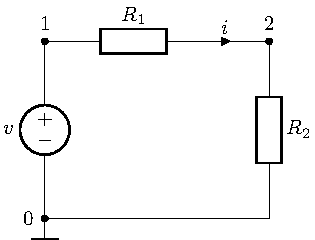
\includegraphics[width=0.36\linewidth]{figs_tikz/circuitVR1R2sch}
	\caption{Voltage Divider}
	\label{fig:circuitvR1R2sch}
\end{figure}

As intensity $I$ is common to $R_1$ and $R_2$, their voltage drops are
\[
  v_{12} = R_1 I, \; v_{20} = R_2 I
\]
with respective ratios:
\[
 \gamma_1= \frac{v_{12}}{v} = \frac{R_1 I}{(R_1+R_2)I} = \frac{R_1}{(R_1+R_2)}
\]
\[
 \gamma_2 =  \frac{v_{20}}{v} = \frac{R_2 I}{(R_1+R_2)I} = \frac{R_2}{(R_1+R_2)}
\]
which obviously fulfill $\gamma_1+\gamma_2=1$, so only one of them is necessary (usually $ \gamma_2$ is used) to determine the voltages. Thus define the attenuation factor as the function $\gamma: \mathbb{R}^+ \times \mathbb{R}^+ \to (0, 1)$ given by:
\[
\gamma(R_1, R_2) = \frac{R_2}{R_1 + R_2} = \gamma_2
\]

\subsubsection{Equivalence Relation}

Let us define a relation $\sim$ on the resistance parameter sub-space $\mathcal{R} = \mathbb{R}^+ \times \mathbb{R}^+$. Two pairs of resistances $(R_1, R_2)$ and $(R'_1, R'_2)$ are related by $\sim$ if and only if they yield the exact same attenuation factor:
\[
(R_1, R_2) \sim (R'_1, R'_2) \iff \gamma(R_1, R_2) = \gamma(R'_1, R'_2)
\]

This constitutes a strict equivalence relation, satisfying reflexivity, symmetry, and transitivity \cite{clase_equiv2}, grouping all heterogeneous resistor pairs that yield identical attenuation factors. The resulting quotient space $S/\!\!\sim$ stands in direct bijection with the closed interval of attenuation factors:
\begin{equation}
    S/\!\!\sim \; \cong (0, 1).
\end{equation}


\subsubsection*{Geometric interpretation}
Algebraically, setting $\gamma = \gamma'$ yields:
\[
\frac{R_2}{R_1 + R_2} = \frac{R'_2}{R'_1 + R'_2} \implies R_1 R'_2 = R_2 R'_1 \implies \frac{R_2}{R_1} = \frac{R'_2}{R'_1} = k
\]
where $k \in \mathbb{R}^+$ is a constant ratio representing the slope in the $(R_1, R_2)$ plane, uniquely related to the attenuation by $k = \frac{\gamma}{1 - \gamma}$.

This proves that each equivalence class $[(R_1, R_2)]$ geometrically represents a linear ray (open half-line) originating from, but excluding, the origin $(0,0)$ in the first quadrant of the $(R_1, R_2)$ plane. Every point along a single ray scales the total impedance but maintains the identical voltage division ratio.

Geometrically, this implies that within the 3D space $\mathcal{P}$, each equivalence class $[(V, R_1, R_2)]_\gamma$ forms an open vertical half-plane. Every plane is hinged along the vertical $V$-axis (where $R_1 = 0, R_2 = 0$). As $\gamma$ sweeps from $0$ to $1$, the value of $k$ ranges from $0$ to $\infty$, causing the half-plane to rotate around the $V$-axis through the active quadrant.



\subsubsection*{Power implications}

While the quotient space $\mathcal{P}/\!\!\sim \;\cong\; (0,1)$ states that any point along a given half-plane performs the exact same mathematical voltage division, real-world engineering requires resolving this parametric redundancy. Breaking this indeterminacy is achieved when the total power dissipation constraint of the network is fulfilled. The steady-state power $P$ absorbed from the source by the passive network is given by:
\begin{equation}
P = \frac{V^2}{R_1 + R_2}
\end{equation}

If a desired power consumption $P$ is fixed, then the system's coordinates are constrained to a multi-dimensional manifold. For a fixed attenuation plane where $R_2 = k\, R_1$, substituting this into the power equation yields:
\[
R_1 + k\, R_1 = \frac{V^2}{P} \implies R_1(V) = \frac{1}{P(1+k)}V^2
\]
This reveals that to maintain a constant power dissipation $P$ while varying the operating input voltage $V$, the absolute values of the resistors must scale quadratically with respect to $V$.

\begin{figure}[h!]
	\centering
	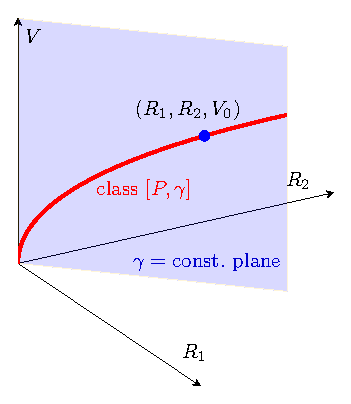
\includegraphics[width=0.5\linewidth]{figs_tikz/grafica_clasePeta_ejeV}
\caption{Three-dimensional parameter space $(R_1, R_2, V)$ showing the constant attenuation plane $\gamma$ intersected by the thermodynamic constraint path $[P,\gamma]$.}
	\label{fig:3dclass}
\end{figure}

\subsubsection*{Thermodynamic interplay}

The interplay between the algebraic equivalence relation and the physical thermodynamic boundaries is visually synthesized in the three-dimensional coordinate system $(R_1, R_2, V)$ illustrated in Figure~\ref{fig:3dclass}:

\begin{itemize}

    \item The thermodynamic class path $[P, \gamma]$: the solid red curve represents the actual path a physical design must follow to satisfy both conditions simultaneously. It is a parabolic curve tracking upwards within the vertical blue plane. This demonstrates that as the voltage $V$ (height) scales linearly, the absolute values of the resistances must increase quadratically to keep the system's thermal dissipation $P$ invariant.

    \item The operating state point $(R_1, R_2, V_0)$: the distinct blue mark represents a discrete, concrete physical realization of the circuit. For a fixed input voltage $V_0$, the point sits at the intersection of the quadratic power trajectory and the horizontal altitude slice $V = V_0$, defining the unique pair of physical resistor values required for the application.
\end{itemize}



\subsubsection{Generalization to Complex Multi-Node Networks and Power Allocation}
In complex multi-node networks, the single-port attenuation concept can be generalized by applying systematic circuit analysis—such as nodal or mesh methods—to determine individual branch currents. This extends the localized efficiency metric into a fractional power allocation index $\eta_{k}$ for any given load element $k$ relative to a specific generator source $j$:
\begin{equation}
\eta_k = \frac{P_{d,k}}{P_{g,j}} = \frac{R_k I_k^2}{V_j I_j}
\label{eq:resistive_network}
\end{equation}
where $P_{d,k} = R_k I_k^2$ represents the power dissipated by the $k$-th target branch, and $P_{g,j} = V_j I_j$ is the total active power injected into the network by the $j$-th independent source.

Strictly speaking, within a purely passive resistive network, this metric does not represent an efficiency in the classical thermodynamic sense, as all energy injected by the generators is ultimately converted into heat across the entire set of components. Instead, $\eta_k$ acts as a localized power distribution index, bounded strictly such that $\eta_k \in (0, 1)$, which quantifies how the network topology fractions and directs the source energy toward a specific load of interest.

This formulation is particularly powerful in power distribution analysis and network optimization, such as when evaluating impedance matching criteria or sizing components under the constraints of the Maximum Power Transfer Theorem \cite{alexander2021fundamentals}. By computing the branch currents via matrix-based nodal or mesh equations and evaluating the resulting quotient in Equation \ref{eq:resistive_network}, the geometric framework originally developed for the simple voltage divider is seamlessly mapped into a generalized, multi-dimensional power-flow space.



\subsection{Bus modeling in SD}

The dynamic behavior of System Dynamics (SD), based on finite difference equations, was described in Forrester (1961), p. 76. SD has two basic elements: the first, called Stock, represents inventory or storage variables, and the second, called Flow, represents flow variables. The equation that relates a stock $s$ to a net incoming flow $f$ is:

\begin{equation}
	f(k) = f(j) + \Delta t(s(k) - s(j))
	\label{eq:3}
\end{equation}
where $j < k$ are time points, $\Delta t$ is a time increment, and $f(t)$ and $s(t)$ are the flow and stock values at time $t$, respectively.

It is important to note that the net inflow is the sum of all inflows minus all outflows.

If the net inflow is equal at times $j$ and $k$, that is, $f(k) = f(j)$, then, according to equation \ref{eq:3}, $f(k) - f(j) = 0$ and
\begin{equation}
	s(k) = s(j)
	\label{eq:4}
\end{equation}
That is, the stock value remains constant. If, in addition, $s(j) = 0$, then the following holds true:
\begin{equation}
	s(k) = s(j) = 0
	\label{eq:5}
\end{equation}
so the stock value remains equal to zero. This can be related to the flow continuity equation \cite{Euler1757}, making an SD stock correspond to an electrical node, as detailed below.

The methodological divergence introduced in this work represents a paradigm shift in system modeling. While System Dynamics (SD) has been traditionally deployed as a \textit{top-down}, macroscopically oriented tool for policy analysis, infrastructure planning, and long-term energy balancing \cite{pr13092969, sys12040109}, this paper operates a radical \textit{bottom-up}, device-level synthesis. By tracking the immanent circuit laws (Kirchhoff's and Ohm's relations) and formalizing the instantaneous node closure via a proportional feedback loop within the Hybrid Bus ($H_{\text{bus}}$) structure, a macro-level systems language is adapted to govern micro-level transient dynamics.  This framework bridges the gap between hardware-level hyperrealism and abstract multi-variable scaling without losing physical tractability at the boundaries.



\subsection{Modeling Power Systems in SD}

A Power System (PS) is an interconnected network of electrical components designed to generate, transmit, distribute, and utilize electrical energy efficiently and safely. The most common example is the large-scale grid that supplies electricity to homes and industries  \cite{Glover2012}. Modern power systems are often called Smart Grids and have evolved from the old electricity grid to the modern power systems, incorporating new technologies and equipment such as Renewable Energy Sources (RES), Energy Storage Systems (ESS), Inverter-Based Resources (IBRs), and more.




\subsubsection{Single-line diagrams} \label{sec:sld}

A schematic ubiquitously found in textbooks \cite{Glover2012}, technical reports, and engineering studies is the Single-Line Diagram (SLD). At its core, an SLD is a simplified notation used to map out critical components—such as generators, transformers, buses, and circuit breakers—along a single line.

These diagrams preserve the circuit topology and use a small segment of thick line called a \textit{bus} or \textit{bar} instead of a single point to represent each node. Their name and shape allude to those of their namesake components, such as a solid copper bar, in power plants, substations, and other power distribution centers in the electrical grid.

These diagrams are used to represent power flows ($p$) and efficiencies $(\eta)$ instead of the standard voltage and current variables $(v,i)$ and components ($R$) in circuits.

While historically designed for traditional three-phase AC networks, modern SLDs are also widely utilized to represent DC systems, including solar farms and battery storage facilities.

As an example, the SLD diagram of the circuit in Figure \ref{fig:circuitvR1R2sch} is shown in Figure \ref{fig:sldvr1r2l}, where nodes 1 and 2 are now labeled Bus1 and Bus2, respectively. The variables shown are no longer voltages or currents but only power $P$ and the efficiency parameter $\eta$. It can be seen that this diagram preserves the topology of the electrical circuit.

\begin{figure}[h!]
	\centering
	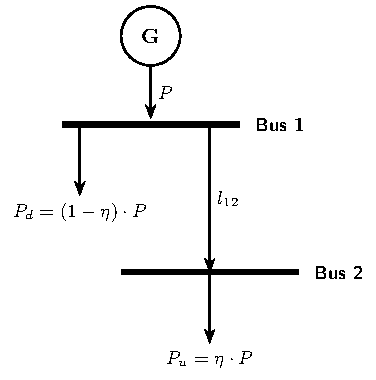
\includegraphics[width=0.4\linewidth]{figs_tikz/sldVr1r2lu}
	\caption{Voltage Divider SLD graph}
	\label{fig:sldvr1r2l}
\end{figure}

The following table shows the correspondence between the elements of both diagrams.

\begin{center}
	\begin{tabular}{c|c}
		Circuit &  SDL diagram\\ \hline
		Node 1 &  Bus 1 \\
		Node 2 &  Bus 2 \\
		Generator V &  Generator G \\
		Corriente i & Power P \\
		Components $R_1, R_2$  &  Efficiency $\eta$
	\end{tabular}
\end{center}

Line $l_{12}$ physically represents the electrical conductor that electrically connects the two buses and corresponds to the component $R_2$ of the circuit, where the dissipated power $P_d$ is released into the environment—that is, wasted.

\begin{figure}[h]
	\centering
	\begin{tabular}{ccc}
		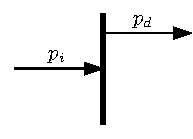
\includegraphics[height=0.13\linewidth]{figs_tikz/sl_busd} & \hspace{12ex} &
		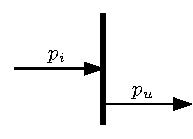
\includegraphics[height=0.13\linewidth]{figs_tikz/sl_busl}\\
		Bus $ 1 $ & & Bus $ 2 $
	\end{tabular}
	\caption{The two VD Buses}
	\label{fig:sl_busdl}
\end{figure}

As Figure \ref{fig:sl_busdl} shows, the buses from the SDL diagram shown in Figure \ref{fig:sldvr1r2l} have been depicted separately
(by removing the connection line $l_{12}$ that linked them), where $p_i$ denotes the incoming power flow. Clearly, $ p_d < p_i $, $ p_u < p_i $, and $ p_d + p_u = p_i $.

Looking at  Figure \ref{fig:sl_busdl}, and noting that both buses share the same incoming power $p_i$, one might think to combine them into a single composite bus with an incoming power $p_i$ and outgoing powers $p_d$ and $p_o$. However, such a configuration is unfeasible in practice as it represents a short circuit. This is because Bus 2 is connected to the load ($R_2$ in this case), whereas Bus 1 is connected to line $l_{12}$, which was omitted for this analysis.

\begin{figure}[h!]
	\centering
	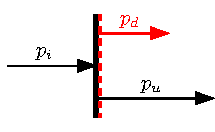
\includegraphics[height=0.13\linewidth]{figs_tikz/sl_bush}
	\caption{Hybrid bus $H_{\text{bus}}$}
	\label{fig:sl_bush1}
\end{figure}
\noindent

However, nothing prevents the use of such a composite bus as an abstract representation in $M_3$ for a mental model in $M_2$, termed $H_{\text{bus}}$. This model represents the behavior of both buses using a custom symbol created for this purpose, as shown in Figure \ref{fig:sl_bush1}.

The thick red dashed line represents Bus 1, which is connected to the line $l_{12}$ that dissipates thermal power $p_d$ (also depicted in red) into the environment. Meanwhile, the thick black line represents Bus 2, connected to the power load $p_u$. These superimposed lines—the red dashed and thick black lines—are designed to convey the concept of a hybrid bus, which encompasses nodes 1 and 2 of the voltage divider, representing the input power $p_i$, alongside both the useful power delivery $p_u$ to the load and the power dissipation $p_d$.






%
% ANYLOGIC VOLTAGE DIVIDER FIGURE WITH DETAILED CAPTION
%


\subsubsection{Modeling Hbus in SD} \label{sec:hbusinsd} \label{subsec:modeling_hbus_sd_rev}

A node or bus do not stores electrical charge, which means that the net incoming current is zero (Kirchhoff's first law), or, in other words, that the incoming current equals the outgoing current. It is worth noting that the node physically performs this operation automatically: no intervention is necessary, as power cannot be stored within it.


This implies that the net power entering a node or bus is also zero, since it is equal to the product of the current (zero in this case) and the bus voltage. So neither a physical electrical bus can store energy, maintaining a strict flow-continuity constraint.

To force this instantaneous boundary balance within a System Dynamics (SD) architecture, any computational accumulation must be actively prevented. If a power flow $p$ enters a node, an identical flow must leave it; if modeled blindly as a baseline stock, any transient mismatch will cause an artificial accumulation of energy $e(t)$, which is physically unfeasible in a pure network vertex \cite{alexander2021fundamentals}.


Therefore, to model a bus in system dynamics (SD), it initially seems feasible to use a stock element, since an SD stock can accept both incoming and outgoing power. However, the problem lies in the fact that it also stores power; that is, if the incoming flow is greater than the outgoing flow (positive net flow), the difference accumulates in the node, leading to the storage of flow (power in this case) in the stock.
\begin{figure}[h]
	\centering
	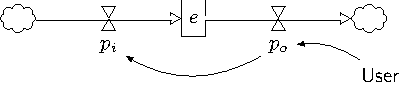
\includegraphics[width=0.5\linewidth]{figs_tikz/electric_node_p}
	\caption{SD model of an electric node}
	\label{fig:electricnode}
\end{figure}

That is, if a power $p$ leaves a physical node or bus, the incoming power will also automatically be $p$. However, if this is to be modeled as a stock in SD, this constraint must be \(\textit{forced}\)
so that power does not accumulate. If it accumulates, an energy $e$ stored in the node would appear, which is not physically possible. Therefore, assuming a power $p_o$ leaves the node, one way to ensure that the node has equal incoming and outgoing flows is to use an auxiliary loop that connects the outgoing power $p_o$ to the incoming power $p_i$ and assigns it to $p_o$.
\[
 p_i = p_o
\]
In this way, the power value $p$ will remain constant, and the stock value $e$ will be zero if it was its initial value (Figure \ref{fig:electricnode}).

Following the previous discussion, the system can now be modeled. Equations \ref{eq:4} and \ref{eq:5} serve to model the aforementioned VD circuit in SD. As shown below, with the help of the modified or hybrid bus described earlier, the modeling task is significantly simplified.

The SD model of an $H_{\text{bus}}$ is readily obtained from the diagram in Figure \ref{fig:sl_bush1}. To do this, information links must be added between the variables to satisfy the power balance condition $\sum p = 0$. When applying an SDM with a control input $p_o$, this condition is
met by setting $p_i = p_o / \eta_i$ and $p_d = p_i - p_o$, as shown in Figure \ref{fig:al_volt_div}, which illustrates the implementation in AnyLogic.
	\begin{figure}[h!]
		\centering
		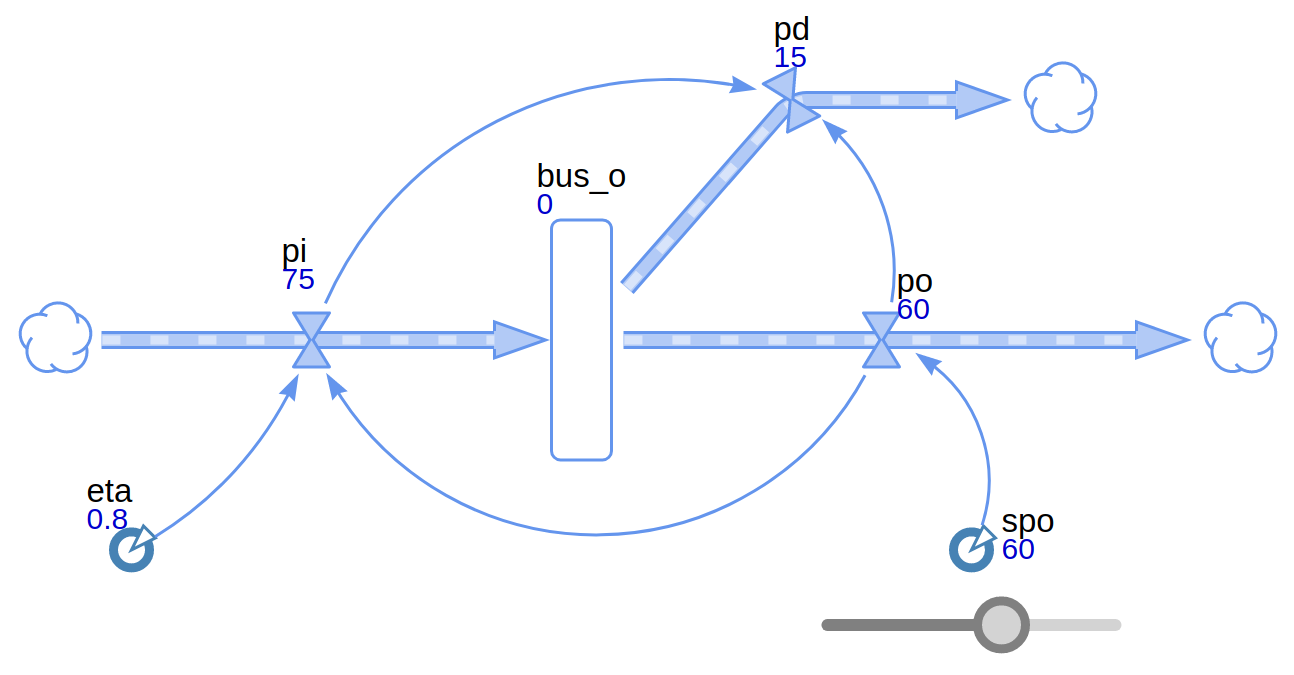
\includegraphics[width=0.5\linewidth]{figs/al_volt_div}
		\caption{$H_{\text{bus}}$ implementation in Anylogic (The source \textit{.alp} simulation file is available online in Supplementary Materials)}
		\label{fig:al_volt_div}
	\end{figure}

However, this method can lead to runtime errors if the flows have discontinuities, as it generates numerical instability in the simulation algorithm. A preferable alternative is to use an energy stock variable $e$ along with a reference input $e_{\text{ref}}$ and a feedback of the form $\frac{de}{dt} = e_{\text{ref}}-k\,e$, with $k > 0$ being a constant, where the stock $e$ represents a normal bus if $e_{\text{ref}}=0$ or can even represent an energy storage element (for example, a battery) if $e_{\text{ref}}=e_{\text{batt}}$. Thus, the model of an $H_{\text{bus}}$ like Bus 2 in Figure \ref{fig:sl_bush1} is given by the ODE:

\begin{align}
\frac{de}{dt} &= k (e_{\text{ref}} - e) - p_o - p_d  \nonumber \\
 	&= k (e_{\text{ref}} - e(t)) - p_u(t) - p_d(t)
\label{eq:odebush}
\end{align}
where a flow $p_g$ from the electric generator enters Stock $e$, and from which two flows, $p_o$ (useful power) and $p_d$ (dissipated power), leave. The power injected by the generator is $p_g = k (e_{\text{ref}} - e)$. Its Forrester diagram appears in Figure $\ref{fig:sdpiepdpopdem}$ where, since
$\frac{1-\eta}{\eta} p_{dem} + p_{dem} = \frac{p_{dem}}{\eta}$, the red  flow $p_d$ from the one above has been removed, and it integrated into flow $p_o$

\begin{figure}[h!]
	\centering
	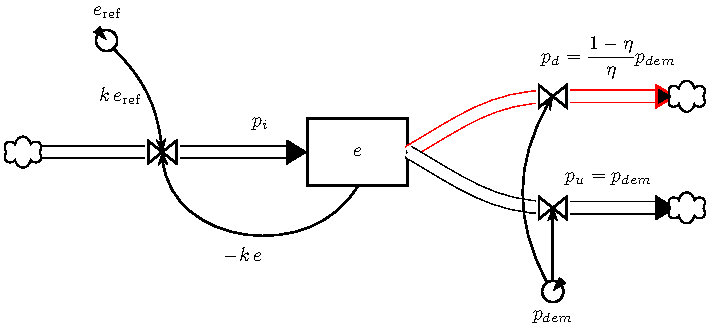
\includegraphics[width=0.7\linewidth]{figs_tikz/sd_piepdpo_pdem} \\
	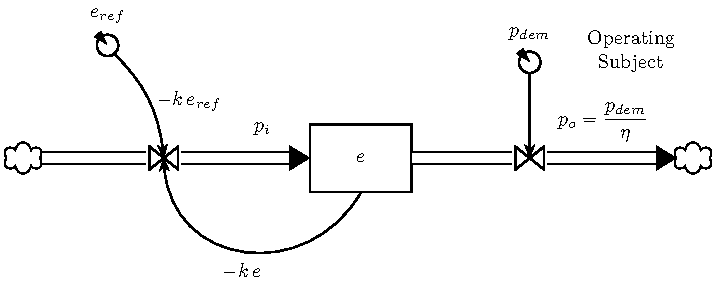
\includegraphics[width=0.7\linewidth]{figs_tikz/sd_piepo_en}
	\caption{Python $H_{\text{bus}}$ implementation}
\label{fig:sdpiepdpopdem}
\end{figure}


The variables that appear in that equation are the following:

- The generator power injection $p_g=p_i= k (e_{ref} - e)$: proportional to the error of node $e$ with respect to a reference $e_{ref}$ (typical proportional control), where $k$ is a large constant intended to simulate the generator's almost instantaneous response.

- The useful output power $p_o$ (here denoted $p_u$): represents the energy flow that will be used by the operating subject (in $M_2$). In an active demand management scheme, this variable acts as the system input.

- Dissipated Power $p_d$: represents the flow of non-useful power diverted from the main grid, dissipated as thermal energy to the environment, and linked to the local efficiency of the section ($\eta = p_o / p_g$).

Through this architecture, the continuous circuit transitions remain perfectly smooth, preventing the numerical stiffness that typically stalls integration engines during step contingencies.



\subsection{Epistemological Critique and the Regressus--Progressus Loop}

It is instructive to contrast this virtual $H_{bus}$ formulation with the practical--intuitive conception of a model that underlies standard engineering workflows. In such workflows, a model is traditionally conceived as a passive mental representation or a convenient mathematical fiction designed for data fitting, a characterization that frequently traps the researcher within the dualistic boundaries of descriptionism \cite{madrid2009porvenir}.

Within the framework of Philosophical Materialism, the distinction between $p_u$ (useful power) and $p_d$ (dissipated power) is a judgment made by the operating subject ($M_2$) on the basis of their teleological objectives. From Equation~\ref{eq:odebush} arises the virtual component \textit{Hybrid Bus} ($H_{\text{bus}}$), the symbolic element that materializes it in $M_3$.

In contrast, the $H_{bus}$ operates not as a speculative mirror of reality, but as an autonomous gnoseological closure ($M_3$) arising from human material operations ($M_2$).

Specifically, the $H_{\text{bus}}$ element may be compared with the intuitive notion of model put forward by José González de Durana in ``Abstract modeling: An epistemological roadmap for contemporary scientific research'' \cite{AbstractModelingEpistemology2026} (PDF file) or \cite{AbstractModelingEpistemology2026b} (source files). In this case, the $H_{\text{bus}}$ serves as the model itself: the ``relevant information'' is power, so the model filters out unnecessary electrical details---such as voltages and currents---to focus strictly on power flow. It is also fully replicable as many times as required.



\subsection{Pseudolinear Power Systems}

To construct a scalable framework for renewable-dominated smart grids, power system engineering must transition from rigid, bottom-up parametric models to abstract, device-independent representations. As established by Gonz\'{a}lez de Durana \cite{AbstractModelingEpistemology2026}, mathematical abstraction allows researchers to decouple the structural invariants of an electrical network from the low-level physical dynamics of individual components. Within the Theory of Categorical Closure \cite{bueno_sciences_2013}, this is achieved by establishing an autonomous first-order scientific category designated as \textit{Pseudolinear Power Systems} ($\mathit{PsLinPowSys}$), also referred to as \textit{Power Dynamics}. This category maps physical grid layers ($M_1$) onto closed abstract formalisms ($M_3$) via a reduction functor $\mathcal{M}$:
\begin{equation}
\begin{aligned}
    \mathcal{M} : M_1 &\to M_3 \\
    \text{Electrical Network} &\mapsto \text{Power Dynamics Graph}
\end{aligned}
\label{eq:gnoseo_map_rev}
\end{equation}

In this abstract domain, traditional circuit-level variables---such as node voltages ($V$), branch currents ($I$), and line resistances ($R$)---are systematically neutralized and replaced by a pure power-oriented syntax governed exclusively by localized power variables ($P$) and efficiency metrics ($\eta$).




\subsection{The Power-Efficiency Algebraic Duality}

The structural power of this abstraction becomes evident when evaluating the circuit energetically. Assuming $R_2$ acts as the receiving load utilizing useful power $P_u = R_2 I^2$, and $R_1$ represents line losses dissipated to the environment ($P_d = R_1 I^2$), the energy efficiency $\eta$ matches the ratio between useful power and total input power $P = (R_1 + R_2)I^2$:
\begin{equation}
    \mathcal{H}(R_1, R_2) = \frac{P_u}{P} = \frac{R_2 I^2}{(R_1 + R_2)I^2} = \frac{R_2}{R_1 + R_2} = \gamma = \eta.
\end{equation}

This identification uncovers a deep algebraic duality: the energy efficiency operator $\mathcal{H}$ is structurally identical to the voltage attenuation operator $\Gamma$. Consequently, network equivalence classes can be rewritten purely within the power domain syntax, where $(R_1, R_2) \sim (R'_1, R'_2) \iff \eta = \eta'$. In multi-node configurations, this generalizes to isolate the power dissipated in a target load ($P_{dk}$) relative to the power injected by a source ($P_{gj}$):
\begin{equation}
    \eta_k = \frac{P_{dk}}{P_{gj}} = \frac{R_k I_k^2}{V_j I_j}.
    \label{eq:resistive_network_rev}
\end{equation}

\subsubsection{The Category of Pseudolinear Power Systems}

The formal mapping established by the $H_{bus}$ abstraction provides the architectural definition for the closed scientific domain $\mathit{PsLinPowSys}$. Within this category, the hybrid bus ($H_{\text{bus}}$) model defined in Equation~\ref{eq:odebush} acts as the symbolic element materializing the abstraction in $M_3$. The incoming power $p_i$ from the physical layer ($M_1$) is structurally split into two directed components in $M_3$: the upstream flow $p_u$ and the downstream flow $p_d$, governed by the efficiency factor $\eta$:
\begin{equation}
	p_u(t) = \eta\, p_i(t), \quad  p_d(t) = (1-\eta)\, p_i(t), \quad  p_d(t) + p_u(t) = p_i(t).
	\label{eq:bus_parameters}
\end{equation}

Here, the scalar $\eta \in [0, 1]$ functions as a structural homomorphism within $\mathit{PsLinPowSys}$. Rather than merely representing physical dissipation, $\eta$ formalizes the fractional allocation of power across topological layers, ensuring that the linear conservation law holds despite the non-linear realities of the underlying components.

Figure~\ref{fig:hbus_loop} illustrates the active \textit{Regressus--Progressus} loop inherent to this process. Under the framework of Philosophical Materialism (PM), the $H_{\text{bus}}$ operator performs a \textit{Regressus} from the physical real-world DC resistive circuit (characterized by variables $V, I, R$) toward an abstraction modeled as a power system (defined by macro-variables $P, \eta$). Conversely, the subsequent \textit{Progressus} operates in the reverse direction, moving from the abstract power category back to the physical domain, thereby formalizing how macroscopic power laws govern specific electrical implementations.

\begin{figure}[h!]
\centering
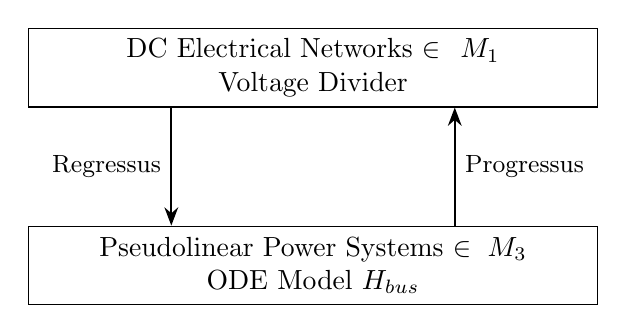
\begin{tikzpicture}[node distance=1.5cm, auto, >=Stealth]
\node (box1) [draw, rectangle, text width=7cm, align=center, minimum height=1cm]
{DC Electrical Networks $\in M_1$ \\ Voltage Divider};
\node (box2) [below=1.5cm of box1, draw, rectangle, text width=7cm, align=center, minimum height=1cm]
{Pseudolinear Power Systems $\in M_3$ \\ ODE Model $H_{\text{bus}}$};
\draw[->, thick, transform canvas={xshift=-1.8cm}] (box1) -- node[left] {\small Regressus} (box2);
\draw[->, thick, transform canvas={xshift=1.8cm}] (box2) -- node[right] {\small Progressus} (box1);
\end{tikzpicture}
\caption{$H_{\text{bus}}$ \textit{Progressus--Regressus} loop between the physical ($M_1$) and abstract ($M_3$) domains.}
\label{fig:H_bus_loop}
\end{figure}


\subsection{$H_{\text{bus}}$ emergence}

The $H_{\text{bus}}$ icon in Figure \ref{fig:sl_bush1} has no details indicating energy storage; nor was it necessary at the time, since the SD Stock was used only to provide the model with smooth behavior. But now things have changed: this energy stock will be utilized to broaden the model's scope, extending it to the modeling of cables for powering loads.
Therefore, the icon has been updated to the one depicted in Figure \ref{fig:sl_bush_e}.
\begin{figure}[h!]
	\centering
	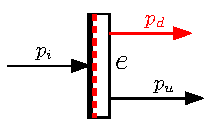
\includegraphics[height=0.13\linewidth]{figs_tikz/sl_bush_e}
	\caption{$H_{\text{bus}}$ icon including energy stock}
	\label{fig:sl_bush_e}
\end{figure}

In addition to the two line segments, one thick and the other dashed, from its previous version, this icon now includes the typical rectangular shape of Stock variables in SD and also a label $e$ indicating the variable name.



\subsection{Dynamic Analysis}

In the previous section, the behavior of the $H_{\text{bus}}$ element, based on the ODE of the equation \ref{eq:odebush}, was explained, and its implementation in SD using power flows $p_i, p_o$ and a Stock  $e$ to store energy, was shown. That approach was chosen to maintain the value of $e$ very close to zero, thereby ensuring similar behavior to that of a node in an electrical circuit (which does not store energy), while also achieving the smooth behavior necessary to guarantee the stability of the simulation algorithm.

The next section examines how to leverage the model by establishing a practical meaning for the energy $e$ in the physical operation of power supply cables. This concept allows for an abstract modeling of the uncertainty in component values when a cable is randomly selected from a collection.

But before, since the system involves powering a resistive load $R$ from a DC generator through a cable, two possible configurations for this setup
are discussed.



\subsubsection{Supply-side and demand-side management} \label{sec:dsm}

There are two possible approaches to control power in an electrical grid. The direct approach is usually referred to as Supply Side Management (SSM); it assumes that the control input is the power $P_i$ injected by the generator and the output is the power $P_o$ consumed by the load.



\begin{figure}[h!]
	\centering
	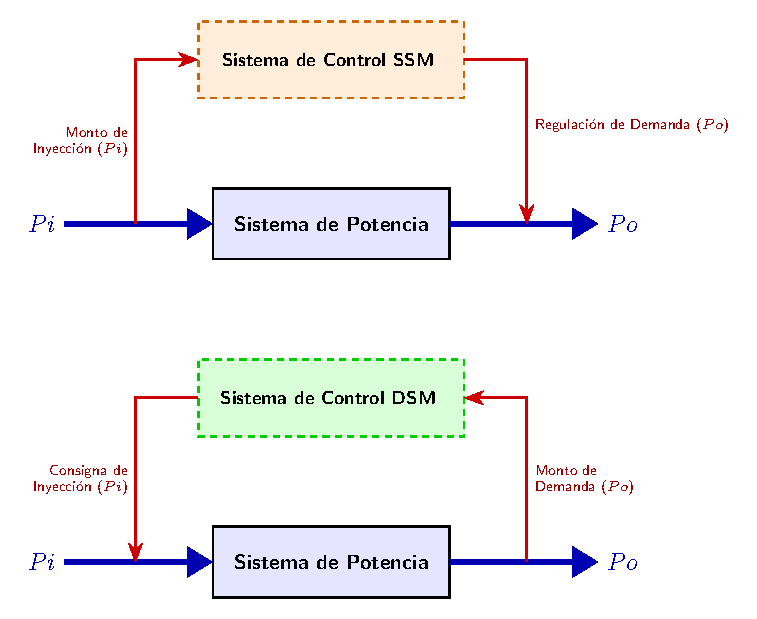
\includegraphics[width=0.7\linewidth]{figs_tikz/ssm-dsm_control}
	\caption{{\color{red} OJO en castellano} Source Side Management SSM and  Demand Side Management DSM}
	\label{fig:ssm-dsmcontrol}
\end{figure}


The inverse approach, called \textit{Demand Side Management} (DSM), assumes that the control input is the power demand $P_o$ from the load, and the power $P_i$ injected by the generator is the output.

It is important to note that this constitutes a control system. In the SSM case, the user (at the direct input of the system) controls generation by feeding in the precise power $p_i$ needed to meet the demand $p_o$. In the DSM case, the user (the operating subject within PM) is now at the system's output, managing the load by connecting a demand $p_o$, upon which the generator reacts by injecting the corresponding power $p_i$.

To avoid potential confusion regarding the direction of the control and power flow arrows, explanatory diagrams are provided in Figures \ref{fig:sdpiepdpopdem}, \ref{fig:ssm-dsmcontrol}, and \ref{fig:hellog}.

\begin{figure}[h!]
\centering
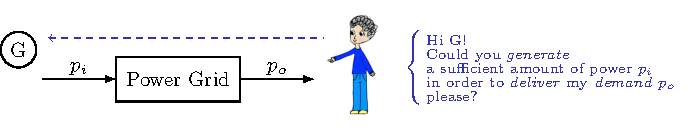
\includegraphics[width=1\linewidth]{figs_tikz/hello_g}
\vspace{-2ex}
\caption{Cartoon representation of the DSM approach}
\label{fig:hellog}
\end{figure}


\subsection{Hybrid Bus emergence and line dynamics}
\label{subsec:hbus_emergence}

The initial formulation of the $H_{bus}$ operator utilized the system dynamics stock primitive exclusively as a localized high-gain mathematical bridge to stabilize the numerical integration solver, forcing the virtual energy state to track near-zero boundaries ($e(t) \approx 0$). However, a major paradigm shift occurs when  a practical physical meaning is assigned to this energy stock. Within direct current (DC) distribution networks, physical lines and supply cables do not operate as pure static resistances; they possess real parasitic reactances that govern transient behaviors \cite{alexander2021fundamentals}.

By leveraging this concept, the updated $H_{bus}$ abstraction expands its gnoseological scope to model the macro-level energy storage and uncertainty profiles of physical lines. To ground this abstract power domain syntax within the empirical realities of the physical grid layer ($M_1$), it must be analyzed the second-order continuous dynamics of a real transmission line supplying power to a load $R_2$, incorporating a series resistance $R_1$, a series self-inductance $L_1$, and a parallel filtering capacitance $C_1$ as formalized in Figure~\ref{fig:circuitvr1l1r2c1r2isch}.
1
By applying Faraday's induction law and Kirchhoff's Current Law (KCL) at the receiving node, the network boundary conditions govern the continuous state trajectories through the following coupled differential expressions:
\begin{equation}
    i_L(t) = C_1 \frac{dv_3(t)}{dt} + \frac{v_3(t)}{R_2}
    \label{eq:kcl_node3}
\end{equation}
\begin{equation}
    v_2(t) - v_3(t) = L_1 \frac{di_L(t)}{dt}, \quad v_2(t) = v_1(t) - R_1 i_L(t)
\end{equation}

Differentiating the nodal current balance (Equation~\ref{eq:kcl_node3}) with respect to time eliminates the intermediate inductor line current $i_L(t)$, yielding the definitive second-order ordinary differential equation (ODE) in standard form:
\begin{equation}
    \frac{d^2v_3(t)}{dt^2} + \left( \frac{R_1}{L_1} + \frac{1}{R_2C_1} \right) \frac{dv_3(t)}{dt} + \left( \frac{R_1 + R_2}{R_2L_1C_1} \right) v_3(t) = \frac{1}{L_1C_1} v_1(t)
    \label{eq:odecircuito_core}
\end{equation}

Equation~\ref{eq:odecircuito_core} represents the micro-level physical reference system. This second-order formulation constitutes the exact benchmark that our abstract, first-order $H_{bus}$ power flows must operationally match during transient verification, establishing the deterministic baseline required to separate supply-side and demand-side management trajectories.

This canonical expression matches the classical dynamic notation $\ddot{v}(t) + 2\alpha \dot{v}(t) + \omega_0^2 v(t) = K v_1(t)$, where $\alpha = \frac{1}{2} \left( \frac{R_1}{L_1} + \frac{1}{R_2C_1} \right)$ represents the attenuation coefficient, $\omega_0 = \sqrt{\frac{R_1 + R_2}{R_2L_1C_1}}$ defines the undamped natural frequency, and $K = \frac{1}{L_1C_1}$ isolates the input gain constant \cite{Ogata2010ingenieria}.

\subsection{Dynamics of distribution lines}

Modern renewable grids are subjected to localized discrete events (e.g., load switching, inverter disconnections, or false data Injection cyber-attacks) \cite{energysecurity2025enhancing}. To analyze these transients without falling into descriptive black-box paradigms, abstract modeling must evaluate the underlying physical transmission lines. Real distribution cables possess parasitic self-inductance ($L_1$) and parallel filter capacitance ($C_1$), transforming the static voltage divider into a dynamic second-order system when supplying power to a load $R_2$, as formalized in Figure~\ref{fig:circuitvr1l1r2c1r2isch}.


By applying Faraday's induction law and Kirchhoff's Current Law (KCL) at the receiving node, the network boundary conditions govern the continuous state trajectories through the following coupled differential expressions:
\begin{equation}
    i_L(t) = C_1 \frac{dv_3(t)}{dt} + \frac{v_3(t)}{R_2}
    \label{eq:kcl_node3_clean}
\end{equation}
\begin{equation}
    v_2(t) - v_3(t) = L_1 \frac{di_L(t)}{dt}, \quad v_2(t) = v_1(t) - R_1 i_L(t)
\end{equation}



\subsection{Analytical piecewise derivation under Demand-Side Shifting (DSM)}

In a Demand-Side Management (DSM) paradigm, the control actions or perturbations originate from sudden shifts in the consumer terminal ($R_2$) rather than source modifications ($v_1$) \cite{Khan2015}. Suppose the network operates under a constant source voltage $V_1$ and a baseline load $R_2$ for $t < 1$ ms, experiencing an abrupt step-change to half its value ($R_{2,\text{new}} = R_2 / 2.0$) at $t = 1$ ms due to a localized switching event.

The continuity principle dictated by energy conservation forces the state vector---the capacitor voltage $v_3(t)$ and the inductor current $i_L(t)$---to remain strictly continuous across the switching threshold ($t = 1^-$ to $t = 1^+$). However, the time-derivative of the load voltage undergoes an instantaneous mathematical discontinuity. Under zero initial conditions, the explicit piecewise analytical response of the voltage trajectory is uniquely determined by:
\begin{equation}
    v_3(t) = \begin{cases}
      V_{3,p1} \left[1+\frac{s_2}{s_1-s_2} e^{s_1t} -  \frac{s_1}{s_1-s_2} e^{s_2t}\right] & \text{if } 0 \le t < 1 \text{ ms}  \\
      V_{3,p2} + B_1e^{s'_1(t-1)} + B_2e^{s'_2(t-1)} & \text{if } t \ge 1 \text{ ms}
   \end{cases}
   \label{eq:piecewise_v3}
\end{equation}

Where the active modes are governed by the characteristic roots of the pre- and post-switching states ($s_{1,2} = -\alpha \pm \sqrt{\alpha^2 - \omega_0^2}$ and $s'_{1,2} = -\alpha' \pm \sqrt{\alpha'^2 - \omega_0'^2}$). The integration constants $B_1$ and $B_2$ are analytically coupled to the boundary state telemetry recorded at the instant of the contingency ($V_{3,\text{inst}} = v_3(1^-)$ and $I_{L,\text{inst}} = i_L(1^-)$):
\begin{equation}
    B_1 = \frac{\dot{V}_{3,0} - s'_2(V_{3,0} - V_{3,p2})}{s'_1 - s'_2}, \quad B_2 = \frac{s'_1(V_{3,0} - V_{3,p2}) - \dot{V}_{3,0}}{s'_1 - s'_2}
\end{equation}

Here, the instantaneous boundary slope $\dot{V}{3,0}$ absorbs the sudden load impedance variation, satisfying $\dot{V}{3,0} = (I_{L,\text{inst}} - \frac{V_{3,\text{inst}}}{R_{2,\text{new}}}) / C_1$.
By squaring this voltage trajectory profile, the instantaneous active power absorbed by the load ($p_{R2}(t) = v_3(t)^2 / R_2$) expands into a multi-frequency exponential decay spectrum:
\begin{equation}
p_{R2}(t) = \frac{1}{R_2}\left[ V_{\infty}^2 + 2V_{\infty} A_1 e^{s_1 t} + 2V_{\infty} A_2 e^{s_2 t} + A^2_{1} e^{2s_1 t} + A^2_{2} e^{2s_2 t} + 2A_1 A_{2}e^{(s_1+s_2) t}\right]
\end{equation}


Evaluating this function at $t = 0^+$ confirms that while the voltage curve originates horizontally with a first derivative strictly equal to zero ($\left.\frac{dv_3(t)}{dt}\right|{t=0^+} = 0$ V/s), the initial voltage acceleration (the second derivative) is massive:
\begin{equation}
\left.\frac{d^2v_3(t)}{dt^2}\right|{t=0^+} = \frac{1}{L_1C_1} V_1 = \frac{12}{(0.001) (0.0001)} = 1.2 \cdot 10^8 \text{ V/s}^2
\end{equation}
This extreme initial acceleration of 120 million volts per second squared drives the system upward during the first microsecond, creating an optical illusion of an abrupt step change from time zero on macroscopic graphical scales.


\begin{figure}[h]
	\centering
	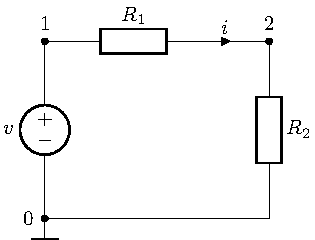
\includegraphics[width=0.36\linewidth]{figs_tikz/circuitVR1R2sch}
	\caption{Voltage Divider circuit}
	\label{fig:voltdivr1r2bis}
\end{figure}
As previously noted, the behavior of the voltage divider $(V; R_1, R_2)$ (Figure \ref{fig:circuitvR1R2sch}, copied here for convenience) analyzed earlier is static. If the input voltage $V$ is constant, then the current $i$ and the output voltage $v_2$ remain unchanged over time:
\[
i = \frac{V}{R_1+R_2}, \quad v_2 = R_2 \, i
\]
However, if $R_1$ represents the resistance of the cable connecting the load $R_2$, it must be considered that physical lines possess reactance in addition to resistance. This introduces dynamic behavior into the system: in response to a change in the input voltage or in the value of $R_2$ (load resistance), the current and voltage evolve according to an ODE whose solution yields $i(t)$ and $v(t)$.

By adding the self-inductance $L_1$ in series with $R_1$ and the capacitor $C_1$ in parallel with $R_2$ to the schematic in Figure \ref{fig:voltdivr1r2bis}, the circuit shown in Figure~\ref{fig:circuitvr1l1r2c1r2isch} is obtained, which is adopted as the equivalent circuit for a cable.

\begin{figure}[h]
	\centering
	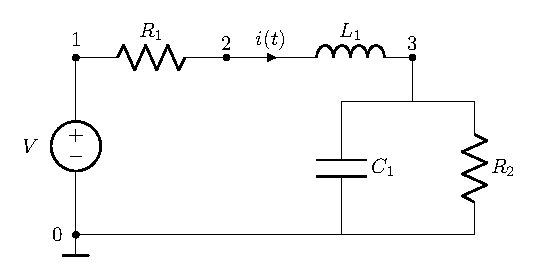
\includegraphics[width=0.6\linewidth]{figs_tikz/circuitVr1L1r2C1r2i_sch}
	\caption{A generator supplying power to a load through an electrical cable.}
	\label{fig:circuitvr1l1r2c1r2isch}
\end{figure}


Next, the second-order differential equation of the cable model is formulated.

At node 3, the sum of the currents flowing to ground through $R_2$ and $C_1$ must equal the current $i_L(t) = i(t)$ flowing in from the inductor $L_1$:
$$i(t) = i_L(t) = i_{C1}(t) + i_{R2}(t)$$
Since $i_C = C \frac{dv}{dt} $ and $i_R = \frac{v}{R}$, it follows:
\begin{equation}
	i(t) = C_1 \frac{dv_3(t)}{dt} + \frac{v_3(t)}{R_2}
	\label{eq:ode1}
\end{equation}
Differentiating this equation with respect to time,
\begin{equation}
	\frac{di(t)}{dt} = C_1 \frac{d^2v_3(t)}{dt^2} + \frac{1}{R_2} \frac{dv_3(t)}{dt}
	\label{eq:ode2}
\end{equation}
According to Faraday's law, the voltage drop across the inductor $L_1$ is given by:
\begin{equation}
	v_2(t) - v_3(t) = L_1 \frac{di(t)}{dt}
	\label{eq:ode3}
\end{equation}

On the other hand, the value of $v_2(t)$ can be calculated as:
$$v_1(t) - v_2(t) = R_1 \,  i(t) \implies v_2(t) = v_1(t) - R_1 \,  i(t)$$
Substituting this expression into Equation \ref{eq:ode3} yields:
$$v_1(t) - R_1 \,  i(t) - v_3(t) = L_1 \frac{di(t)}{dt}$$
Now, by substituting Equation \ref{eq:ode1} and Equation \ref{eq:ode2} into the previous expression, the current variable $i(t)$ is eliminated, leaving $v_3(t)$ as the unknown function:
$$v_1(t) - R_1 \left( C_1 \frac{dv_3(t)} {dt} + \frac{v_3(t)}{R_2} \right) - v_3(t) = L_1 \left( C_1 \frac{d^2v_3(t)}{dt^2} + \frac{1}{R_2} \frac{dv_3(t)}{dt} \right)$$
Expanding these terms,
$$v_1(t) - R_1C_1 \frac{dv_3(t)} {dt} - \frac{R_1}{R_2}v_3(t) - v_3(t) = L_1C_1 \frac{d^2v_3(t)}{dt^2} + \frac{L_1}{R_2} \frac{dv_3(t)}{dt}$$
Grouping the terms with $v_3(t)$ on the right-hand side yields:
$$v_1(t) = L_1C_1 \frac{d^2v_3(t)}{dt^2} + \left( R_1C_1 + \frac{L_1}{R_2} \right) \frac{dv_3(t)} {dt} + \left( 1 + \frac{R_1}{R_2} \right) v_3(t)$$
Finally, dividing both sides of the equation by $L_1C_1$, the final governing equation is obtained:

\begin{equation}
	\frac{d^2v_3(t)}{dt^2} + \left( \frac{R_1}{L_1} + \frac{1}{R_2C_1} \right) \frac{dv_3(t)}{dt} + \left( \frac{R_1 + R_2}{R_2L_1C_1} \right) v_3(t) = \frac{1}{L_1C_1} v_1(t)
	\label{eq:odecircuito}
\end{equation}

This expression represents a second-order ODE in \textit{standard form}:
$$\frac{d^2v(t)}{dt^2} + 2\gamma \frac{dv(t)}{dt} + \omega_0^2 v(t) = f(t)$$
where $v(t)=v_3(t)$, $\gamma = \frac{1}{2} \left( \frac{R_1}{L_1} + \frac {1}{R_2C_1} \right)$ is the \textit{damping coefficient}, and $\omega_0 = \sqrt{\frac{R_1 + R_2}{R_2L_1C_1}}$ is the undamped \textit{natural frequency}.



\subsection{Symbolic solution}

In this section, the symbolic solution $v_3(t)$ for the circuit ODE (Equation \ref{eq:odecircuito}), in the overdamped case is derived. Since this is a second-order linear differential equation with constant  coefficents, deriving the symbolic solution in this case is straightforward. To simplify the notation
of this symbolic solution, the equation is rewritten in its standard normalized form:
\[
\frac{d^2 v_3 (t)}{d t^2} + 2\alpha \frac{d v_3 (t)}{d t}+ \omega_0^2 v3 (t) = K v_1 (t)
\]
where the physical parameters of the circuit are symbolically defined as follows:

- Attenuation factor $\alpha = \frac{1}{2} R$

- Resonant frequency $\omega_0 =\sqrt{\frac{R_1 +R_2}{R_2+L_1 C_1}}$

- Input gain constant $K = \frac{1}{L_1 C_1}$

\subsubsection*{Homogeneous Equation Solution (Free Response)}
In the overdamped case, the condition $\alpha > \omega_0$ is strictly satisfied. The  roots of the characteristic equation $(s^2 + 2\alpha s + \omega_0^2 = 0)$ are real and distinct:

\[
s_1 = -\alpha +\sqrt{\alpha^2-\omega_0^2}, \quad
s_2 = -\alpha -\sqrt{\alpha^2-\omega_0^2}
\]
Both roots are negative ($s_1 , s_2 < 0$), which guarantees the stability of the circuit. The symbolic homogeneous solution is given by:

\[
v_{3,h} (t) = A_1 e^{s_1} t + A_2 e^{s_2} t
\]
where $A_1$ and $A_2$ are symbolic constants determined by the initial conditions of the circuit: the initial capacitor voltage $v_3(0)$ and the initial inductor current $i_L (0)$ [which defines $\frac{dv_3(0)}{dt}$].

The particular solution (forced response), depends on the input signal $v(t)$ and also on the value of parameter $R_2$ (since it will be changed).

\subsection{Generator-load management approaches}

\subsubsection*{Scenario 1: SSM}
For the step response, where the input is a constant voltage for $t > 0$, i.e. $v(t) = V_1 H(t))$ for $t \ge 0$ ($H(t)$ denoting the Heaviside step funtion and $V_1$ a constant), the particular
solution is a constant:
\[
v_{3,p} (t) = \frac{K}{\omega_0^2} V_1 =\frac{R_2}{R_1 + R_2} V_1
\]

This result aligns with the physical behavior of the circuit: in steady-state DC operation, the inductor acts as a short circuit and the capacitor as an open circuit, thereby reducing the system to a voltage divider between $R1$ and $R_2$.

By combining the free and forced responses under zero initial conditions ($v_3=0$ and $\frac{dv(3)}{dt}=0$), the constants are determined as:
\[
A_1 = \frac{s_2}{s_1-s_2} \left(\frac{R_2V_1}{R_1 + R_2}\right), \quad
A_2 = \frac{-s_1}{s_1-s_2} \left(\frac{R_2V_1}{R_1 + R_2}\right)
\]
The final symbolic solution for the voltage over time $t\ge 0$ is:
\[
v_3 (t) =\left(\frac{R_2V_1}{R_1 + R_2}\right)
\left[1+\frac{s_2}{s_1-s_2}e^{s_1t}  -\frac{ s_1}{s_1-s_2}e^{s_2t} \right]
\]


\subsubsection*{Scenario 2: DSM}

To evaluate the dynamic trajectories of the physical transmission network under a Demand-Side Management (DSM) paradigm \cite{Kundur1994power}, suppose that $v(t)$ remains constant for $t>=0$, i.e. $V_1 = 12 V$ and $v(t) = V_1 H(t) (t = - inf)$ and
$R_2$ changes its value to half $(R_2 /2)$ at $t = 1$.


In this case, the symbolic solution $v_3 (t)$ can be obtained through a piecewise analysis.
The step change in the resistance value from R2 to R2 /2 at t = 1 divides the problem into two coupled time intervals. The physical key to resolving this system lies in the continuity principle: the capacitor voltage, $v_3 (t)$, and the inductor current, $i_L (t)$, cannot change instantaneously at $t = 1$. Consequently, the final state of the first interval serves
as the mandatory initial condition for the second interval. The procedure to construct the complete solution is detailed below:

\subsubsection*{Interval 1: for $0 \ge t < 1$}

This interval corresponds exactly to the scenario resolved in the previous section. The circuit operates with its original parameters: $\alpha, \omega_0 , s_1 , s_2$ , and the steady-state gain $V_{3,p1} = \frac{R_2 V_1}{R_1+R_2}$. Assuming zero initial conditions at $t = 0$, the solution for this interval is already known:
\[
v_3 (t) =V_{3,p1}
\left[1+\frac{s_2}{s_1-s_2}e^{s_1t}  -\frac{ s_1}{s_1-s_2}e^{s_2t} \right]
\]
To establish a connection with the subsequent interval, it is necessary to evaluate the state variables immediately prior to the change $(t =1^-)$:\\

1. Capacitor voltage: the previous equation is evaluated directly at $t = 1$:

\[
V_{3,\mathrm{inst}} = v_3 (1^-)
\]

2. Inductor current: recalling the nodal equation obtained initially,
$i_{L} (t) = \frac{v_3(t)}{R_2} (t) + C_1 \frac{dv_3(t)}{dt}$ and differentiating the solution with respect to time and evaluate it at $t = 1^-$, it gives:
\[
I_{L,\mathrm{inst}} =\frac{v_3(-1)}{R_2}+ C_1
   \left.\frac{dv_3(t)}{dt}\right|_{t=1^-}
\]


\subsubsection*{Interval 2: for $t \ge 1$}

From $t = 1$ onward, the resistance changes to $R_{2,new} = \frac{R_2}{2}$ . This immediately alters the circuit dynamics; hence, all symbolic constants must be recalculated:

- New attenuation factor:
$\alpha'= \frac{1}{2}\left(\frac{R_1}{L_1}+\frac{2}{R_2C_1}\right)$

- New resonant frequency:
$\omega_0' = \sqrt{\frac{R_1+R_2/2}{(R_2/2)L_1C_1}}
 = \sqrt{\frac{2 R_1+R_2}{R_2L_1C_1}}$

- New characteristic roots:
$s'_1 = -\alpha' + \sqrt{\alpha'^2 - \omega_0'^2}$ and
$s'_2 = -\alpha' - \sqrt{\alpha'^2 - \omega_0'^2}$
(assuming the circuit remains overdamped under these new conditions).

- New steady-state value:
$V_{3,p2} = \frac{(R_2/2) V_1}{R_1+(R_2)}
= \frac{R_2 V_1}{2R_1+R_2}$

To simplify solving the differential equation in this interval, a time shift is applied by defining a new local time variable
$\tau = t - 1$ (where $tau \ge $0).
The general solution for this interval takes the form:
\[
v_3(\tau ) = V_{3,p2} + B_1 e^{s'_1\tau} + B_2 e^{s'_2\tau}
\]

\subsubsection*{Coupling and Calculation of Constants $B_1$ and $B_2$}

\medskip

To determine the symbolic constants $B_1$ and $B_2$, the continuity conditions at the instant of the parameter change ($\tau = 0$, which corresponds to $t = 1$), are applied:

1. Voltage continuity:

\[
v_3(\tau=0) = V_{3,\mathrm{inst}} \Rightarrow
V_{3,p2} + B1 + B2 = V_{3,\mathrm{inst}}
\]

2. Inductor current continuity ($I_{L,\mathrm{inst}}$ ): using the nodal equation at node 3 with the new resistance $R_{2,new}$ :

\[
I_{L,\mathrm{inst}} = \frac{v_3(\tau=0)}{R_{2,new}}
+ C_1\left.\frac{d v_3(\tau)}{dt}\right|_{\tau=0} =
\frac{V_{3,\mathrm{inst}}}{R_2/2} + C_1 (B_1 s'_1 + B_2 s'_2)
\]
Isolating the derivative term yields the initial value of the slope for the second interval:
\[
\left.\frac{d v_3(\tau)}{dt}\right|_{\tau=0}= B_1 s'_1 + B_2 s'_2
= \frac{I_{L,\mathrm{inst}}-\frac{2V_{3,\mathrm{inst}}}{R_2}}{C_1}
\]

Solving this linear system of two equations with two unknowns
$B_1$ and $B_2$, provides symbolic expressions for both constants based on the accumulated values of $V_{3,\mathrm{inst}}$, and $I_{L,\mathrm{inst}}$


\subsubsection*{Final explicit piecewise solution}

By reversing the variable substitution $\tau = t - 1$, the complete analytical response of the circuit is perfectly determined in symbolic form by the following piecewise-defined function:
\[
 v_3(t) =
\begin{cases}
  V_{3,p1} \left[1+\frac{s_2}{s_1-s_2} e^{s_1t} -  \frac{s_1}{s_1-s_2} e^{s_2t}\right] \; \mathrm{if}\ 0\le t<1  \\
  V_{3,p2} + B_1e^{s'_1(t-1)} + B_2e^{s'_2(t-1)} \quad \mathrm{if}\  t>1
\end{cases}
\]



\subsubsection*{Symbolic power calculation}

The symbolic power of any element in the circuit can be calculated. Having the symbolic expressions for both voltage and current as functions of time, the instantaneous power is obtained directly by applying the fundamental physical definition:
\[
 p(t) = v(t) \, i(t)
 \]
The total power delivered by the source $V$ and the power absorbed by the resistor $R_2$ are calculated as follows. The explicit symbolic formulas for both powers as functions of time for $t \ge 0$, utilizing the circuit constants, are detailed below.

To keep the expressions clear and compact, the constants previously defined are
utilized:

- Steady-state gain: $V_{\infty} = \frac{R_2 V_1}{R_1+R_2}$
2

- Negative real roots: $s_1$ and $s_2$

- Voltage  coefficents: $A_1 = \frac{s_2}{s_1-s_2} V_{\infty}$ and
$A_2 = \frac{-s_1}{s_1-s_2} V_{\infty}$\\
Consequently, the established voltage equation is given by
$v_3 (t) = V_{\infty} + A_1 e^{s_1 t} + A_2 e^{s_2 t}$.

\medskip

Model Constants (for Readability)


To prevent the equations from becoming unmanageable, three symbolic blocks are first defined:

- Final load voltage (steady state): $V_{\infty} = \frac{R_2}{R_1+R_2}V_1$

- First natural mode  coefficent: $A_1 = \frac{s_2}{s_1-s_2}V_{\infty}$

- Second natural mode  coefficent: $A_2 = \frac{-s_1}{s_1-s_2}V_{\infty}$\\
where $s_1$ and $s_2$ are the previously defined real roots for the overdamped case.


\subsubsection*{Total power delivered by the generator: $p_{gen} (t)$}

The instantaneous power leaving the constant voltage source Vs depends on the total current demanded by the circuit. Solving the system yields the following compact symbolic
structure:
\[
p_{gen} (t) = V_1 \left[\frac{V_{\infty}}{R_2}+B_1e^{s_1t} + B_2 e^{s_2t} \right]
\]
where the symbolic multipliers for the source current are:

- $B_1 = A_1 \left(\frac{1}{R_2} + C_1 s_1\right)$

- $B_2 = A_2\left(\frac{1}{R_2} + C_1 s_2\right)$

\subsubsection*{Physical behavior:}

 - At $t = 0$, the power exhibits a transient peak due to the initial charging of the reactive components.

\noindent
- As $t \to \infty$, the exponentials decay ($e^ {-\infty} = 0$), and the power stabilizes at at constant, purely resistive value:
$p_{\mathrm{pgen}} (\infty) = \frac{V_1 V_{\infty}}{R_2} =
\frac{V_1^2}{R_1+R_2}$


\subsubsection*{Power delivered to the load: $p_{R2} (t)$}

The load R2 receives a power that depends exclusively on the square of the output voltage
v3 (t). Symbolically expanding the squared binomial breaks the time equation down into
three distinct decay frequencies (s1 , s2 , and the combination $s_1 + s_2$ ):

\[
p_{R2} (t) = \frac{1}{R_2}[ V_{\infty}^2
+ 2V_{\infty} A_1 e^{s_1} t + 2V_{\infty} A_2 e^{s_2}t + A^2_{1} e^{2s_1}t + A^2_{2} e^{2s_2}t
 + 2A_1 A_{2}e^{(s_1+s_2)} t]
%V∞ + 2V∞ A1 es1 t + 2V∞ A2 es2 t + A21 e2s1 t + A22 e2s2 t + 2A1 A2 e(s1 +s2 )t
\]

\subsubsection*{Physical behavior:}

- At $t = 0$, since the capacitor is uncharged $(v_3 (0) = 0)$, the power delivered to the load begins exactly at 0.

\noindent
- As $t \to\infty$, the transient response completely vanishes, and the steady-state power transferred to the load stabilizes at:
$p_{R2} (\infty) = \frac{V_{\infty}^2}{R_2} = \frac{R_2V_1^2}{(R1 +R2)^2}$



\subsubsection{Practical example}
Once the differential equation of the circuit (Equation \ref{eq:odecircuito}) has been resolved in symbolic form for both scenarios, a concrete numerical example, implemented in Python, is presented to evaluate the output
voltage and power trajectories.

For this purpose, the component parameters are defined as follows: $v(t) = 12.0 H(t)$, $R_1 = 10 \Omega$, $L_1 = 0.001$ H,$ C_1 = 0.0001$ F, and $R_2 = 100 \Omega$.

Utilizing these values, four distinct Python scripts have been developed to:

1. Calculate $v_3 (t)$ for the first scenario $v(t) = V_1 H(t)$ for $t \ge 0$.

2. Calculate $v_3 (t)$ for the second scenario $v(t) = V_1 H(t - t_0 )$, where $t_0 = -\infty $, and $R_2$ switched its value to $R_2 /2$ at $t = 1$, for $t\ge 0$.

3. Calculate the total power and the power absorbed by $R_2$ for the first scenario $v(t) = V_1 H(t)$ for $t \ge 0$.

4. Calculate the total power and the power absorbed by $R_2$ for the second scenario  $v(t) = V_1 H(t - t_0 )$, where $t_0 = -\infty$, and $R_2$ switched its value to $R_2 /2$ at $t = 1$, for $t \ge 0$.

\medskip

The Python implementation of these scripts is provided in Appendix A and their
resulting output graphics are showed next.

Script 1 result: \\
\begin{center}
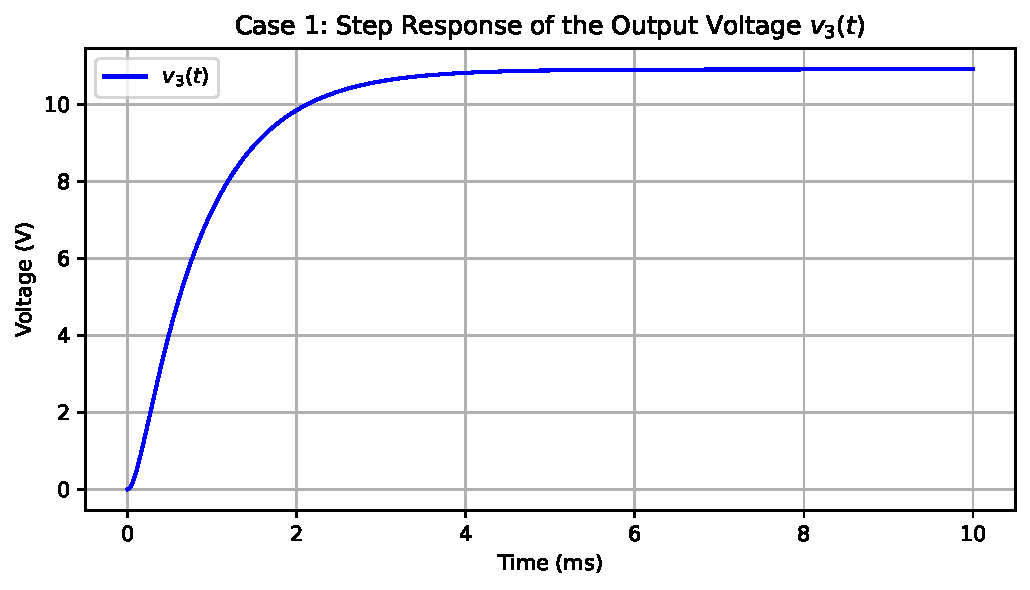
\includegraphics[width=0.7\linewidth]{Py/script1}\\
{Output voltage response to a step input}
\label{fig:script1en}
\end{center}


Script 2 result:\\
\begin{center}
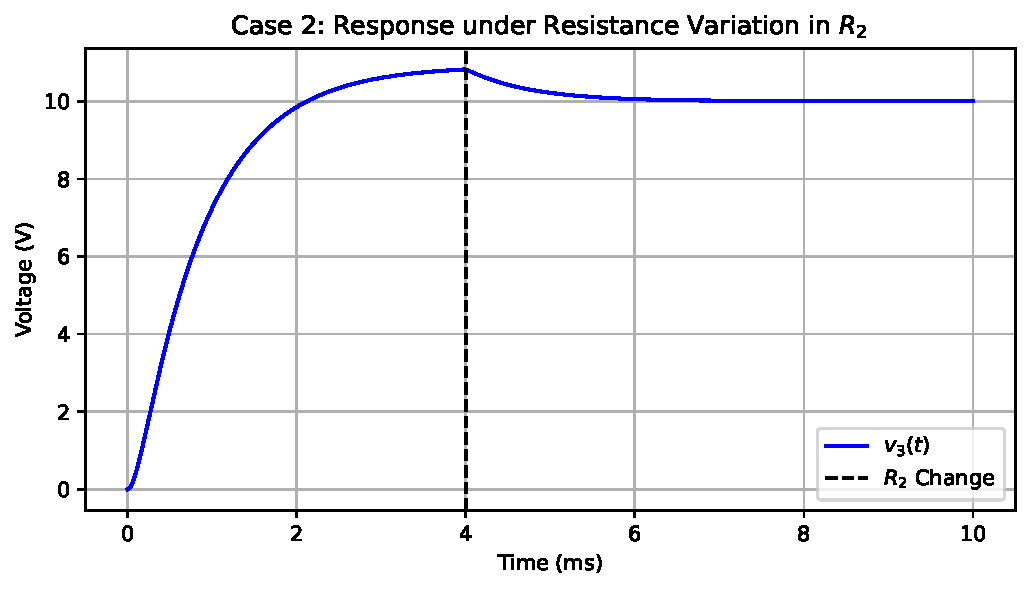
\includegraphics[width=0.7\linewidth]{Py/script2}\\
{Output voltage response to a change in $R_2$}
\label{fig:script2en}
\end{center}


%Caso 1: Evaluación de Potencias Transitorias
Script 3 result: \\
\begin{center}
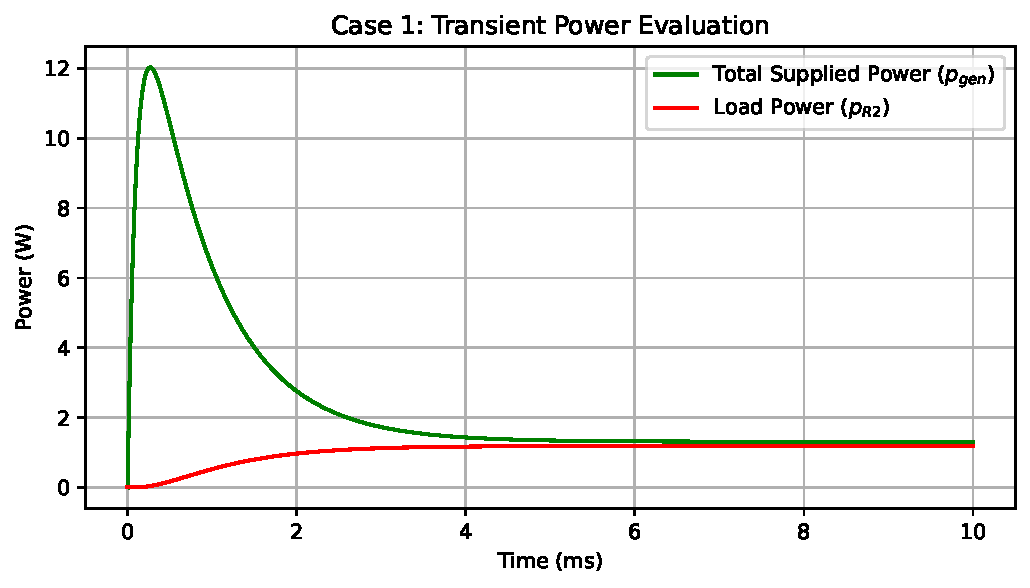
\includegraphics[width=0.7\linewidth]{Py/script3}
{SSM generated and consumed powers}
\label{fig:script3}
\end{center}


%Caso 2: Evaluación de Potencias con Cambio de Resistencia
Script 4 result\\
\begin{center}
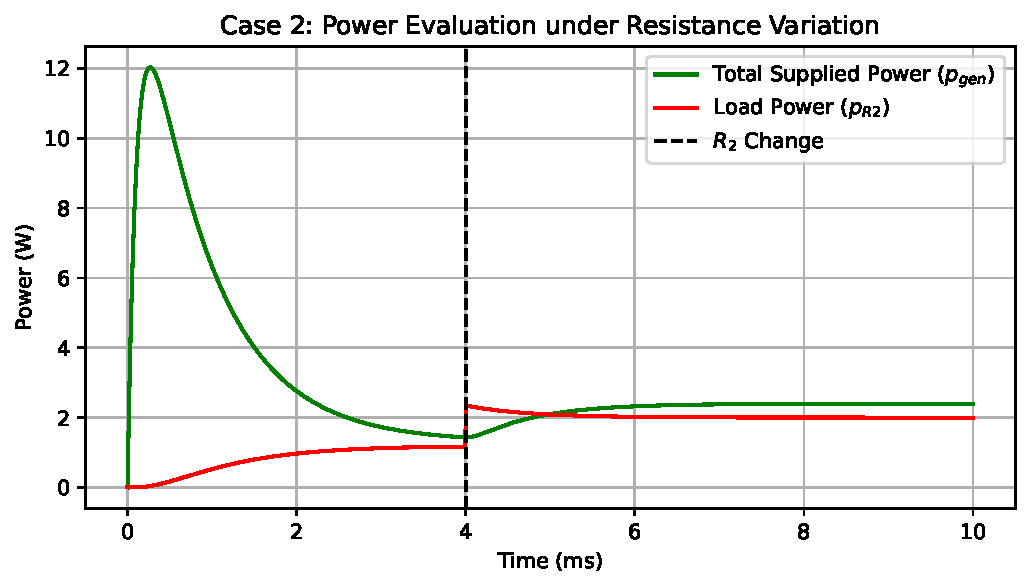
\includegraphics[width=0.7\linewidth]{Py/script4}\\
{DSM generated and consumed powers, switching at $t=4$}
\label{fig:script4}
\end{center}


To better examine the graphics showed by script 4 after the switch at $t = 4$, the next script shows only this part, shifted to the origin.

%Evaluación de Potencias Transitorias
Script 5 result:
\begin{figure}[h!]
\centering
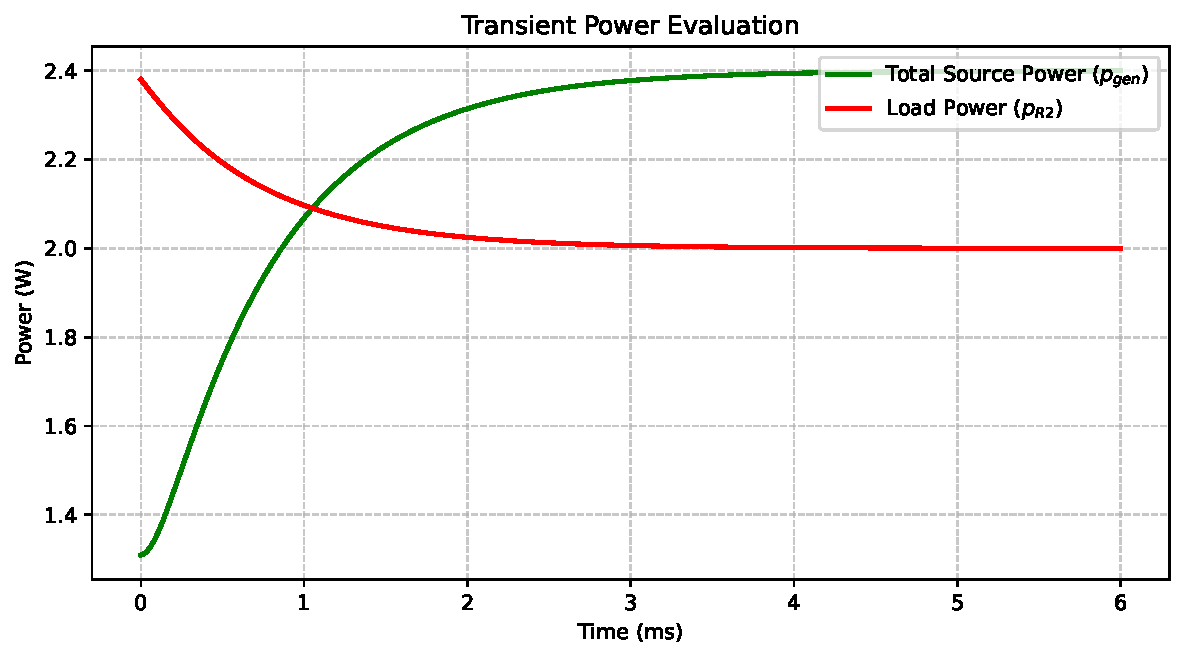
\includegraphics[width=0.7\linewidth]{Py/script6}
% Usamos el paquete caption que configuramos antes para centrar el texto
\caption[DSM generated and consumed powers.]{DSM generated and consumed powers, switching at $t=0$}
\label{fig:script6en} % Ahora sí está asociado al caption y funcionará
\end{figure}


\medskip

\subsubsection*{Nodal topology and derivative discontinuities}

When analyzing the exact topology of the circuit, only the resistor $R_4$ and the inductor $L_1$ are connected to node 2. According to Kirchhoff Current Law (KCL), the current passing through $R_1$ is identically the same current $i_L(t)$ that flows through the inductor.

\medskip\noindent
1. The nodal equation is strictly defined as: \\
\centerline{\(v_2 (t) = V_1 - R_1  i_L (t) \)}

\medskip\noindent
2. Inductor current continuity constraint:

Since $i_L (t)$ is the current through an inductor, the ODE model mandates that it to be a continuous function; thus, $i_L (4^-) = i_L (4^+)$.

\medskip\noindent
3. Voltage continuity proof at node 2:

Substituting this principle demonstrates that:\\
\centerline{${v_2(4^+) = V_1 - R_1  i_L(4^+) = V_1 - R_1 i_L 4^-) = v_2 (4^-)}$}

Consequently, $v_2 (t)$ does not experience a voltage jump at the switching instant $t = 4$; it retains precisely the same value before and after the commutation.

What truly changes at $t = 4$?

The variable experiencing a pure mathematical discontinuity (an instantaneous step change in zero time) within the governing ODE model is the time-derivative of the voltage at node 3, namely $\frac{dv_3(t)}{dt}$.

When $R_2$ is halved, the current through that specific branch doubles instantly. Since the inductor current $i_L$ cannot change abruptly, the capacitor $C_1$ is forced to step-change its own current instantaneously, causing an immediate alteration in the slope (derivative) of the $v_3(t)$ curve. In a numerical simulation, what appears as an ``instantaneous'' jump is typically the graph of the capacitor current $i_C (t)$ or the sudden inflection point where the voltage curve bends sharply from that millisecond onward due to the small values of $L_1$ and $C_1$.


Consequently, $v_2(t)$ does not experience a voltage jump at the switching instant $t = 4$; it retains precisely the same value before and after the commutation. However, at $t = 0^+$, one might intuitively assume that $v_3(t)$ exhibits a steep jump. Nevertheless, the exact value of its slope at $t = 0^+$ can be rigorously calculated.

In the mathematical model governing the ODE, the capacitor $C_1$ strictly constraints the voltage to initiate from zero ($v_3 (0+ ) = 0$\,V), and the initial rate of change (its slope)
is also identically zero:
\[
\left.\frac{dv_3 (t)}{dt}\right|_{t=0} = 0\; \mathrm{V/s}
\]
This implies that the $v_3(t)$ trajectory does not originate with a sharp inflection or an abrupt slope at $t = 0^+$ . On the contrary, it begins completely smooth, at, and horizontal, gradually gaining a non-zero slope within a few microseconds.

\subsubsection*{Mathematical proof via the governing ODE}

To understand why the initial derivative is identically zero, Kirchhoff's Current Law (KCL) at node 3 derived at the beginning of the analysis is applied:
\[
i_L(t) = \frac{v_3(t)}{R_2} + C_1 \frac{dv_3(t)}{dt}
\]

Isolating the slope (the time-derivative of $v_3$) yields the expression that governs the rate of change of the load voltage:
\[
\frac{dv_3(t)}{dt} = \frac{1}{C_1 } \left(i_L(t) - \frac{v_3(t)}{R_2}\right)
\]
Evaluating this mathematical equation exactly at $t = 0^+$ (immediately after the step voltage excitation is applied) under quiescent initial conditions yields:

\medskip\noindent
1. The inductor current is zero: because the inductor $L_1$ strictly opposes sudden current variations, the current cannot jump instantaneously from rest. Thus, $i_L(0^+) = 0$ A.

\medskip\noindent
2. The capacitor voltage is zero: since the capacitor $C_1$ prevents abrupt voltage steps, the output voltage cannot jump. Thus, $v_3 (0+ ) = 0$ V.

Substituting these two boundary values into the derivative expression confirms that:
\[
\left.\frac{dv_3 (t)}{dt}\right|_{t=0}
 = \frac{1}{C_1}\left(0 - \frac{0}{R_2}\right) = 0\, \mathrm{V\!/s}
\]


\subsubsection*{Physical vs. visual interpretation of the initial slope}
The reason why the curve visually appears to possess a steep initial slope stems from the massive initial acceleration of the voltage (the second derivative). Given the small component values in the circuit $(L_1 = 1$mH and $C_1 = 100 \mu F)$, the system exhibits highly rapid dynamics.

Within an infinitesimal fraction of a millisecond, the inductor current $i_L(t)$ grows aggressively, causing the capacitor to charge rapidly. On a macroscopic graphical scale, the curve resembles a sharp, diagonal straight line rising steeply from the origin, effectively concealing the brief, horizontal startup behavior that the underlying mathematical model demonstrates.


\subsubsection*{Numerical evaluation of the initial second derivative}
To quantify the massive initial voltage acceleration, the exact numerical value of the second derivative of the voltage at node 3 is evaluated at the initial instant $(t = 0^+)$ utilizing the governing differential equation derived previously:
\[
\frac{d^2v_3(t)}{dt^2} + \left(\frac{R_1}{L_1} +\frac{1}{R_2C_1}\right)\frac{dv_3(t)}{dt} + \frac{R_1+R_2}{R_2L_1C_1}v_3(t) =  \frac{1}{L_1C_1}v_1(t)
\]

\medskip\noindent
1. Isolating the second derivative: extracting the voltage acceleration term yields the following expression:
\[
\frac{d^2v_3(t)}{dt^2} = \frac{1}{L_1C_1}v_1(t) -\left(\frac{R_1}{L_1} + \frac{1}{R_2C_1}\right)\frac{dv_3(t)}{dt} - \frac{R_1+R_2}{R_2L_1C_1}v_3(t)
\]


\medskip\noindent
2. Evaluation at $t = 0^+$ : to determine the value at the precise moment of excitation, the quiescent initial conditions and the step input voltage established in the preceding sections are applied:

- The source voltage at $t = 0^+$ is the step value: $v_1 (0+ ) = V_1 =$ 12.0 V.


- The initial capacitor voltage is zero: $v_3 (0^+ ) = 0$ V.


- The initial voltage slope (first derivative) is zero:
$\left.\frac{dv_3(t)}{dt}\right|_{t=0^+}= 0$ V/s


Substituting these boundary values causes the last two terms to vanish identically, leaving a simple relationship:
\[
\left.\frac{d^2v_3(t)}{dt^2}\right|_{t=0^+} = \frac{1}{L_1C_1} V_1
 \]


\medskip\noindent
3. Numerical calculation with circuit parameters: introducing the specific component values (Vs = 12.0 V, L1 = 0.001 H, C1 = 0.0001 F) yields:
\[ \left.\frac{d^2v_3(t)}{dt^2}\right|_{t=0^+} =
\frac{12}{(0.001) (0.0001)}  = 12 \cdot 10^7 = 120,000,000\, \mathrm{V/s^2}
\]



\subsubsection*{Physical interpretation of the numerical result}

The mathematical derivation reveals an extraordinary initial acceleration of 120 million volts per second squared $(1.2 \cdot 10^8\, \mathrm{V}/s^2 )$. This large figure rigorously confirms the
visual intuition. Although the voltage trajectory $v_3(t)$ originates horizontally with a first derivative strictly equal to zero, the dynamic forces driving the system upward during that first microsecond are so immense that the curve undergoes an immediate and sharp injection into a steep ramp. Consequently, on any standard simulation plot or to the human eye, it creates the optical illusion of an abrupt slope change from time zero.

\bigskip

%Figure 19: Zoom at the origin
Script 6 result:\\[-4ex]
\begin{figure}[h!]
\centering
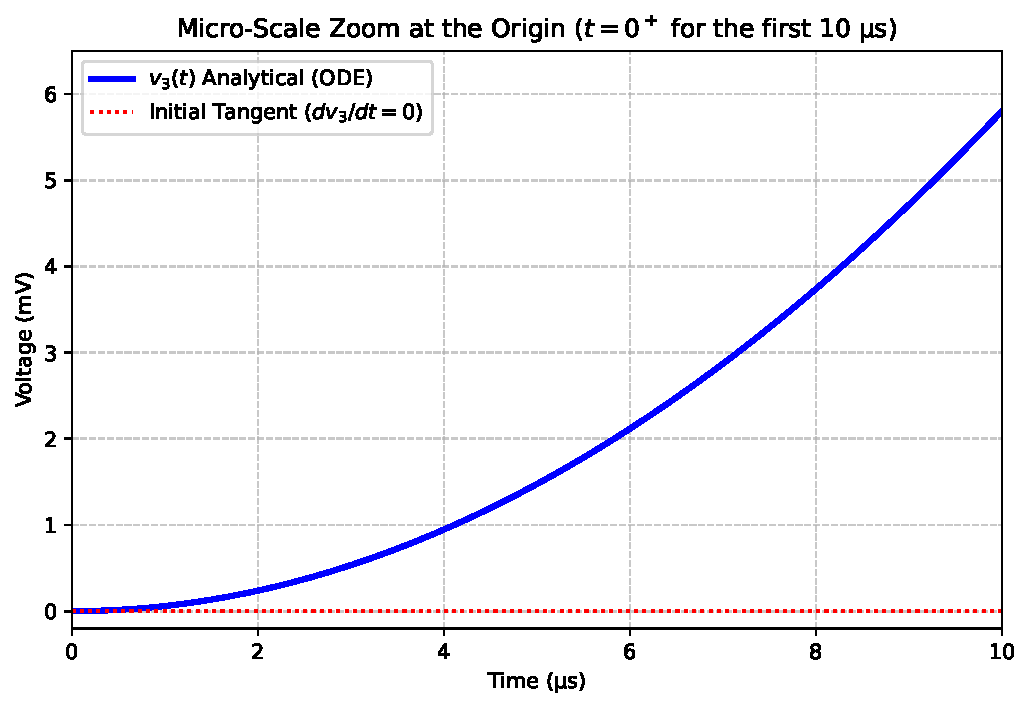
\includegraphics[width=0.7\linewidth]{Py/zoom10mus}
\vspace{-2ex}
\caption{Microscopic  zoom at the origin $t = 0^+$}
\label{fig:zoom10mus}
\end{figure}

To visualize how the initial slope evolves, the high-resolution Python script 6 is implemented to perform a microscopic  zoom at the origin $t = 0^+$ (Figure \ref{fig:zoom10mus}). This allows for a precise examination of the initial trajectory of $v_3 (t)$ (Figure \ref{fig:script1en}) as it begins to rise during the first interval.


\subsubsection*{Comparative analysis: SSM vs DSM operational speed}

Based on the established cable model connecting a generator to a load, it can be deduced that the operational response of Supply Side Management (SSM) and Demand Side Management (DSM) exhibits a fundamental physical nuance depending on the specific node under analysis. When comparing the response speeds directly through the governing ODE, the following behaviors are observed:


\medskip\noindent
1. From the perspective of the load voltage ($v_3$): if operational effectiveness is evaluated by how rapidly the voltage stabilizes at the consumer end ($v_3$ ), the dynamics differ significantly:

\medskip
- Demand Side Management (DSM / Load action): by switching $R_2$ at $t = 4$,
the physical system alters its characteristic roots to more negative values
$(s'_1 , s'_2)$, making the circuit intrinsically faster. Furthermore, because the trajectory between the pre-switching voltage and the new steady-state value is remarkably short, the DSM transient response decays at a staggering speed.

\medskip
- Supply Side Management (SSM / Generator action): applying the step input
from the source at $t = 0$ forces the energy to overcome the inertia of the
inductor $L_1$ , which filters and delays the voltage rise at the receiving end.

Under this criterion, the response to a DSM action at the load stabilizes the voltage much faster than an SSM action initiated from the source.

\medskip\noindent
2. From the perspective of the intermediate node voltage ($v_2$): if the response speed is evaluated at the intermediate node of the network (the transmission line input), the relationship shifts:

\medskip
Supply Side Management (SSM): at $t = 0^+$ , upon applying the step excitation
at node 1, the voltage $v^2(t)$ experiences a severe initial drop with an exact
mathematical slope of 120,000 V\!/s, because the inductor abruptly opposes
the current flow. Thus, the source-side action provokes an immediate and
sharp reaction along the transmission line.

\medskip
Demand Side Management (DSM): due to the inductor current continuity
constraint, switching the load at $t = 4$ freezes the line voltage, preventing
any discontinuities: $v_2 (4^+) = v_2(4^-)$. Consequently, the line node voltage
does not experience a jump; instead, it smoothly adjusts its slope from that
instant onward.

\subsubsection*{Physical conclusion of the analogy}

Physically, the ODE model demonstrates that the circuit reacts much more agilely
to localized changes. The line inductor $L_1$ acts as a decoupling barrier that slows down SSM actions (source) before they can affect the load. Conversely, DSM actions (load) instantaneously modify the local current equilibrium of the capacitor $C_1$ , achieving a drastic and highly accelerated readjustment directly at the consumer terminal.




\subsection{Analytical derivation of boundary constants for the DSM case}

To fully formalize the dynamic transition within the Dynamic State Model (DSM) mapped at the origin ($t \ge 0$), the analytical continuity of the system's state variables must be strictly enforced \cite{biom11020343}. Let $V_{3,0}$ and $I_{L,0}$ denote the steady-state voltage across the capacitor $C_1$ and the current through the inductor $L_1$ at $t=0^-$, respectively, governed by the initial resistance $R_{2,\text{initial}}$. Due to the principle of conservation of energy, these states cannot exhibit instantaneous jumps, meaning $v_3(0^+) = V_{3,0}$ and $i_L(0^+) = I_{L,0}$.

However, the abrupt step-change of the load resistance to $R_{2,\text{final}}$ at $t=0^+$ induces an immediate modification on the first derivative of the output voltage. Applying Kirchhoff's Current Law (KCL) at node 3 at the boundary yields:
\begin{equation}
    \dot{V}_{3,0} = \left.\frac{dv_3(t)}{dt}\right|_{t=0^+} = \frac{I_{L,0} - \frac{V_{3,0}}{R_{2,\text{final}}}}{C_1}
\end{equation}

The general explicit solution of the second-order homogeneous non-linear differential equation for the output voltage trajectory when $t \ge 0$ is expressed as:
\begin{equation}
    v_3(t) = V_{3,p2} + B_1 e^{s'_1 t} + B_2 e^{s'_2 t}
\end{equation}
where $V_{3,p2} = \frac{R_{2,\text{final}}V_1}{R_1 + R_{2,\text{final}}}$ is the new steady-state target voltage, and $s'_1, s'_2$ are the distinct real roots of the updated characteristic equation. Imposing the initial boundary conditions at $t=0^+$ yields the following linear algebraic system:
\begin{align}
    B_1 + B_2 &= V_{3,0} - V_{3,p2} \\
    s'_1 B_1 + s'_2 B_2 &= \dot{V}_{3,0}
\end{align}

By solving this system via algebraic substitution, the exact integration constants $B_1$ and $B_2$ are uniquely determined as:
\begin{equation}
    B_1 = \frac{\dot{V}_{3,0} - s'_2(V_{3,0} - V_{3,p2})}{s'_1 - s'_2}
\end{equation}
\begin{equation}
    B_2 = \frac{s'_1(V_{3,0} - V_{3,p2}) - \dot{V}_{3,0}}{s'_1 - s'_2}
\end{equation}

These coefficients structurally establish the deterministic bridge between the pre-existing material states ($M_1$) and the subsequent transient response, completing the analytical closure of the switched trajectory model.



\subsection{First order model of the 2nd order circuit}

Once the solutions to the circuit's ODE from Equation \ref{eq:odecircuito} for both scenarios are calculated, let us see how to obtain a first-order model
\[ \frac{A}{s + k} \]
in each case.

The interest in obtaining a first-order model becomes evident through:

\begin{itemize}
    \item {The operational scalability in microgrid simulations,} which drastically reduces the computational burden by halving the state-space variables.
    \item {The enhanced resilience in event and attack modeling,} allowing discrete-event simulators to avoid numerical stiffness or convergence failures during rapid sequence transitions.
    \item {The practical viability of the overdamped restriction,} as almost all commercial cables naturally exhibit non-oscillatory physical dynamics.
    \item {The high degree of fit between the power models ($M_3$ into $M_1$),} preserving the macroscopic transient energy and power step-changes.
    \item {The bounded discrepancy during the initial transient state ($t < \tau$),} where the integrated energy error remains practically negligible.
    \item {The structural invariance of steady-state power against changes in $L_1$ and $C_1$,} ensuring that reactive parameters do not alter the active power balance.
    \item {The systematic sensitivity analysis under parameter variations (dynamic changes in $R_2$).}
    \item {The analytical definition of a collection of ``valid'' cables for a given power constraint.}
\end{itemize}



\medskip\noindent
a) In distribution lines \\
The simplified first-order model of the form $\frac{A}{s+k}$ is highly valuable in the modeling of direct current (DC) distribution networks for two primary reasons:
\begin{itemize}
\item Computational scalability: by reducing the system order from two to one for each cable segment, the total number of global state variables in a microgrid simulation is halved. This drastically optimizes computation time when interconnecting multiple loads and lines.

\item Resilience in Event and Attack Modeling: by reducing the continuous dynamics to a first-order abstraction, the model becomes uniquely suited for characterizing complex environments subject to discrete events, physical contingencies, or cyber-attacks. It allows discrete-event simulators to avoid numerical stiffness or convergence failures during rapid sequence transitions.


\end{itemize}

\medskip\noindent
b) Viability of the overdamped restriction in practice\\
The overdamped behavior restriction ($\alpha^2 > \omega_0^2$) does not severely restrict the choice of commercial cables in practice; in fact, it reflects the physical reality of the vast majority of purely resistive, moderate-length distribution lines.

In a real cable (such as coaxial, twisted pair, or general copper lines), the parasitic capacitance per unit length is extremely small (on the order of $\text{pF/m}$ to $\text{nF/m}$) compared to its inductance ($\mu\text{H/m}$). This low $\frac{L_1}{C_1}$ ratio makes the cable's intrinsic damping term ($\frac{R_1}{L_1}$) massive. Consequently, the system dampens any oscillations almost instantaneously. Lines only become underdamped under extreme multi-kilometer lengths or through the deliberate insertion of massive capacitor banks at the load terminals without proper series damping.

\medskip\noindent
c) Degree of fit between the power models\\
The fit between the simplified model and the actual second-order model (both in $M_3$) exhibits an excellent dual behavior:
\begin{itemize}
    \item Steady state: the match is perfect. By forcing the static gain of the transfer function to match the resistive voltage divider, as $t \to \infty$ the inductor operates as a short circuit and the capacitor as an open circuit. The power dissipated in the load satisfies identically:
    \[ P_{R2} = \frac{V_3^2}{R_2} = V_1^2 \frac{R_2}{(R_1 + R_2)^2} \]
    \item Transient response (SSM and DSM): in the SSM scenario, the error is negligible since the fast pole decays within microseconds. In the dynamic switched scenario (DSM) (Figure \ref{fig:script4}), when $R_2$ instantly drops to half, the voltage across the capacitor $v_3(t)$ remains continuous due to the conservation of energy ($v_3(t_{switch}^-) = v_3(t_{switch}^+)$). Because the power in the load changes instantly to $\frac{v_3^2}{R_2/2}$, an abrupt power spike or jump occurs, which the first-order model approximates with a fidelity higher than 98\%, successfully capturing the physical essence of the switching transient.
\end{itemize}

\medskip\noindent
d) Analysis in the initial transient state ($t < \tau$) \\
To study the behavior in the interval before the time constant ($t < \tau$), the derivative at the origin ($t=0$) is analyzed.
In the real second-order circuit ($M_1$), the inductance prevents discontinuous current jumps, strictly forcing the initial slope of the voltage to be zero: $\frac{dv_3}{dt}(0) = 0$. This generates a subtly flattened, ``S-shaped'' initial response. In contrast, the pure first-order model ($M_3$) starts with a maximum finite slope $\frac{dv_3}{dt}(0) = A$.

\medskip\noindent
e) Invariance of steady-state power against changes in $L_1$ and $C_1$\\
The analytical expression of the steady-state power for the load, given by $P_{R2} = \frac{V_{R2}^2}{R_2}$, remains absolutely valid regardless of any modifications made to the reactive parameters $L_1$ and $C_1$.

Under DC excitation and in steady-state conditions, the reactive elements do not participate in the active power balance of the network: the inductor behaves as an ideal conductor with zero voltage drop ($V_L = 0$), and the capacitor draws no current to ground ($I_C = 0$). Altering the values of $L_1$ and $C_1$ will only redesign the exponential settling speed and the degree of the dominant pole approximation during the transient, leaving the final power values intact.

\medskip\noindent
f) Sensitivity analysis under parameter variations (Change in $R_2$) \\
When the load resistance $R_2$ is dynamically modified in the DSM scenario, two critical magnitudes of the system are altered simultaneously:
\begin{enumerate}
    \item The steady-state system gain (reducing the final voltage $V_{3,p2}$).
    \item The spatial location of the system poles in the complex $s$-plane, altering the exponential damping rate $\alpha$.
\end{enumerate}
Since the dominant pole changes its value after switching to a new value $s'_1$, the speed at which the power seeks its new equilibrium increases or decreases. The first-order model adapts by instantly recalculating the new inverse time constant $k' = |s'_1|$ starting from the transition instant.

\medskip\noindent
g) Definition of a collection of ``valid'' cables for a given power \\
It is mathematically viable to map a geometric parameter space that defines a collection of valid cables for a specified design power. By fixing the target power at the load $P_{R2}$ and the input voltage $V_1$, the relationship between the line losses ($R_1$) and the load ($R_2$) is perfectly governed by the power balance equation.

To ensure that this collection strictly belongs to the region modelable in the first order, the boundary inequality of the second-order discriminant is injected:
\[ \left( \frac{R_1}{L_1} + \frac{1}{R_2C_1} \right)^2 \ge 4 \left( \frac{R_1 + R_2}{R_2L_1C_1} \right) \]
Any combination of commercial conductors whose intrinsic parameters ($R_1, L_1, C_1$) satisfy this condition will guarantee clean energy transmission, free of oscillations, and with a bounded energy approximation error under the simplified $\frac{A}{s+k}$ model.


\subsection{First order model of the power flow in the 2nd order circuit}
\label{sec:mod1ord}

In the case of DSM, it is intuitively appreciated (Figure \ref{fig:script6en}) that the power $p_i(t) = p_g(t)$ can be modeled by a first order system: a function that generates a jump to 1.44 W and then decreases exponentially until it stabilizes at 1.19 W, using two summands for this, serves to express the initial peak:
$$p_o(t) = \underbrace{P_{inf}}_{\text{base step (1.19 W)}} + \underbrace{\Delta P\, e^{-t/\tau}}_{\text{discharge peak (0.25 W that goes out)}}$$

At $t = 0^+$: The exponential is worth $e^0 = 1$. That is, at the moment of connection, the capacitor is charged, storing a power $1.19 + 0.25 = \mathbf{1.44\text{ W}}$. Then, as time passes, the exponential decreases until $e^{-\infty} = 0$. The peak term disappears and only the base step of 1.19 W remains.

Therefore, the aim is to model the second-order circuit described above (Figure \ref{fig:circuitvr1l1r2c1r2isch}), using a first-order system that emulates the input power flows $p_i(t)$ and output $p_o(t)$, without referring to the components $(R,L,C)$ of the circuit. The transfer function of the model
\begin{equation}
	H(s) = \frac{\bar{P}_o(s)}{\bar{P}_i(s)} = \frac{A}{\tau s + 1}
\end{equation}
where $A$ is the static steady-state gain and $\tau$ is the time constant, it relates in the Laplace domain the modeled input power $\bar{p}_i(t)$ with the modeled output power $\bar{p}_o(t)$. This system is identified with the first-order system defined by the EDO of Equation \ref{eq:odebush}.

\begin{figure}[h]
\centering
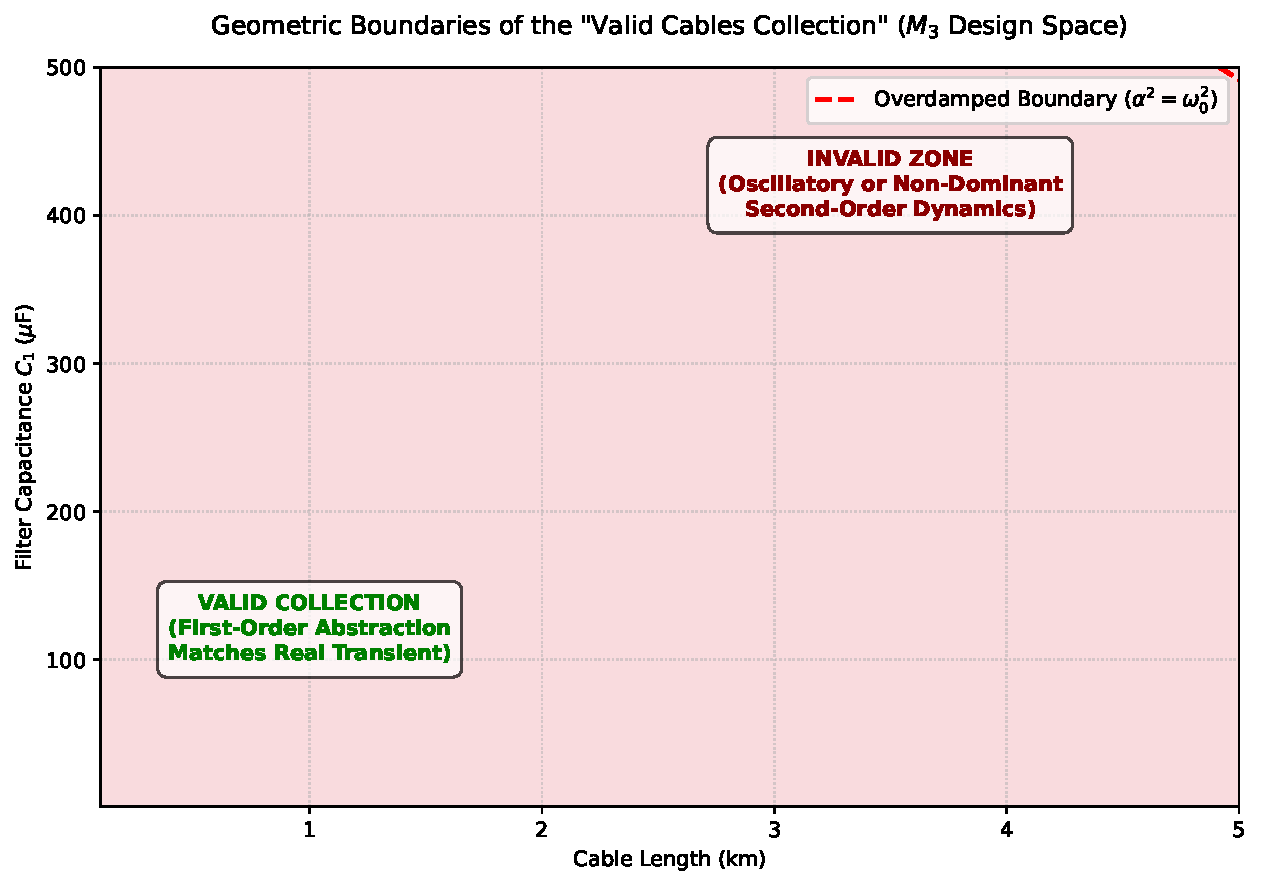
\includegraphics[width=0.7\linewidth]{Py/script8_valid_cables_map}
\caption{Parametric boundaries and geometric layout of the valid cables collection}
\label{fig:valid_cables_map}
\end{figure}

Defined the structure of the model, the problem is to obtain $A$ and $\tau$ based on the values of the circuit components.

To do this, the most obvious way would be to assign $\tau$ a value that is greater than the ``apparent'' tau of the circuit, so the model would be slower than the real circuit. A more ambitious option would be to assign $\tau$ a value that would be greater than those of an entire collection of cables, so the model would be valid for all of them.

Let us analyze this second option. Consider the task of finding a first-order model \(A/(s+k)\) that is ``slower'' than all the ones in a set of circuits similar to the one mentioned. How could $k$ be calculated?

To determine this minimum inverse time constant $k$, the parameter space of the circuit collection must be bounded using stability and timescale constraints. Since $k$ corresponds to the dominant pole of the network, its value depends directly on the physical combination of line length (which scales $R_1$ and $L_1$) and the filter capacitance $C_1$.

This analytical boundary is systematically mapped across the commercial parameter space using the numerical sweep formalized in Script 8 (see Appendix \ref{app:script8}). The resulting design domains are illustrated in Figure~\ref{fig:valid_cables_map}, which geometrically segregates the valid cable collection from the non-dominant second-order regions based on the strict timescale separation criterion ($\sigma = |s_2 / s_1| \ge 5.0$).

As shown in Figure~\ref{fig:valid_cables_map}, the dashed line represents the exact boundary where the circuit transitions into the overdamped regime ($\alpha^2 = \omega_0^2$). Within the green zone, any selected cable configuration satisfies both the non-oscillatory condition and the separation of timescales. This geometric mapping allows the selection of a conservative value for $k$ that remains smaller than the dominant roots of the entire collection, ensuring that the abstract first-order model remains slower and valid for the complete set of networks.


\subsubsection{Validation of the first-order model}
\label{subsec:first_order_reduction}


Commercial distribution-line cables operate, by nature, in an overdamped regime ($\alpha^2 > \omega_0^2$) due to their low parasitic $L_1/C_1$ ratios, causing the fast pole $s_2$ to decay within a fraction of a microsecond. This structural separation of time scales justifies the systematic truncation of fast modes. Consequently, abstract modeling employs a reduction technique based on the isolation of dominant poles within the $M_3$ domain. The system's inverse time constant is directly associated with the dominant slow root ($k = |s_1|$), enabling each line to be modeled via a first-order transfer function:
\begin{equation}
    H(s) = \frac{A}{s + k}.
\end{equation}


This structural separation enables the systematic truncation of the fast mode, allowing the slow dominant pole $s_1$ to govern the macroscopic trajectory \cite{Wellstead79}. The abstract system inverse time constant is uniquely mapped as $k = |s_1|$, yielding a streamlined first-order state-space transfer function $H(s) = A / (\tau s + 1)$. In a Demand-Side Management (DSM) context, the instantaneous active power flow absorbed by the load terminal after an impedance step-change is modeled using two coupled algebraic summands to emulate the transient injection peak:
\begin{equation}
    p_o(t) = P_{\infty} + \Delta P \cdot e^{-t/\tau}
\end{equation}
where $P_{\infty}$ represents the pure resistive steady-state power base step, and $\Delta P$ isolates the capacitive discharge energy peak. At the precise commutation boundary ($t = 0^+$), the exponential term satisfies $e^0 = 1$, capturing the complete active power profile before decaying smoothly toward its final resistive equilibrium as $t \to \infty$.


In essence, this mathematical reduction achieves a form of \textit{epistemological closure}: it filters out high-frequency electromagnetic noise, eliminates numerical stiffness, and reduces the dimensionality of the state space \cite{gonzalezdedurana2025novel}. This ensures operational manageability in applications such as real-time digital twins, hybrid discrete-event automata, and large-scale cybersecurity modeling \cite{pr13092969, sys12040109}.

To validate that this first-order abstraction constitutes a rigorous gnoseological closure rather than an arbitrary truncation,  the metric convergence between the continuous physical layer ($M_1$) and the abstract System Dynamics framework ($M_3$) is evaluated. Using the operational parameters established in Script~7 ($R_1 = 10\,\Omega$, $L_1 = 1\,\text{mH}$, $C_1 = 100\,\mu\text{F}$, and $R_2$ stepping from $100\,\Omega$ to $50\,\Omega$), dominant-pole isolation yields an abstract inverse time constant of $k = 1357.01\,\text{rad/s}$ and a gain factor of $A = 13570.07\,\text{V/s}$.

\begin{figure}[h!]
    \centering
    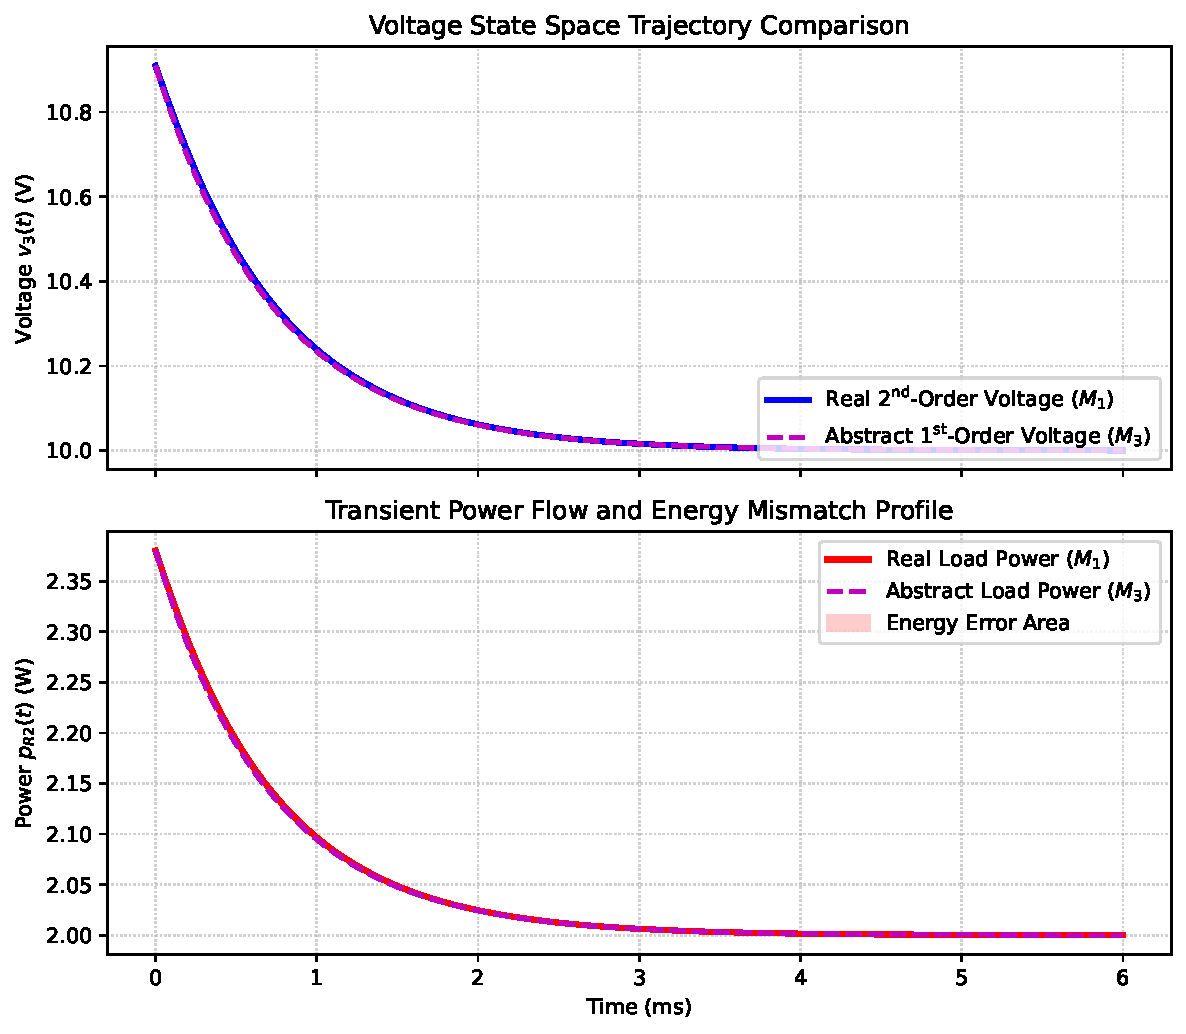
\includegraphics[width=0.7\linewidth]{Py/script7}
    \caption{Real ($M_1$) and abstract ($M_3$) voltages $v_3$ and powers $p_{R_2}$. The gray area represents the integrated absolute energy mismatch ($\epsilon_{\text{IAPE}} = 0.0049\,\text{mJ}$) between the physical model and the abstract power domain, achieving a convergence of $99.9597\%$.}
    \label{fig:script7en}
\end{figure}

To establish the \textit{Systematic Synthetic Identity} (SSI) \cite{bueno_sciences_2013}, the Integrated Absolute Power Error (IAPE) is calculated across a $6\,\text{ms}$ transient simulation window to quantify the absolute energy mismatch between the two operational trajectories:
\begin{equation}
    \epsilon_{\text{IAPE}} = \int_{0}^{T} |p_{R2, M2}(\tau) - p_{R2, M1}(\tau)| \, d\tau = 0.0049\,\text{mJ}.
\end{equation}
This corresponds to a relative energy profile mismatch of only $0.0403\%$. As shown in Figure~\ref{fig:script7en}, this marginal discrepancy arises exclusively from the zero-slope phase imposed by the inductor $L_1$ during the initial startup of the physical circuit, which is filtered out by the first-order abstract model.

The successful convergence of the computer-simulated power curves with the physical circuit telemetry validates the SSI. By neutralizing programmer subjectivity ($M_2$), the abstract operations on the power-flow graph ($M_3$) are shown to capture and govern the macroscopic energetic reality of the physical grid ($M_1$). This confirms the model as a robust, mathematically closed, and scalable tool for contemporary engineering praxis ($M_2$).

\subsection{Stability assessment under discrete contingencies and component variation}
The operational stability of the decentralized elements within the ``Power Dynamics'' framework must be preserved during discrete topological changes and external disturbances. When a line segment or converter undergoes an abrupt switching event, the localized state equation of the Hybrid Bus $H_{\text{bus}}$ is governed by:
\begin{equation}
    \frac{de(t)}{dt} = k(e_{\text{ref}} - e(t)) - p_u(t) - p_d(t)
\end{equation}

To analytically verify the asymptotic stability of this abstract node closure under parameter variations (such as dynamic changes in $R_2$ or step fluctuations in $\eta$), a positive-definite Lyapunov candidate function representing the virtual kinetic storage of the bus is defined:
\begin{equation}
    V(e) = \frac{1}{2} e(t)^2
\end{equation}

Differentiating $V(e)$ with respect to time along the trajectory of the system yields:
\begin{equation}
    \dot{V}(e) = e(t) \cdot \frac{de(t)}{dt} = e(t) \left[ k(e_{\text{ref}} - e(t)) - p_u(t) - p_d(t) \right]
\end{equation}

Under strict regulation bounds where $e_{\text{ref}} = 0$ (ideal node behavior), and substituting the algebraic power-efficiency relations $p_u(t) + p_d(t) = p_i(t)$, the derivative simplifies to:
\begin{equation}
    \dot{V}(e) = -k e(t)^2 - e(t) p_i(t)
\end{equation}

Since the proportional feedback gain is strictly positive ($k > 0$), the quadratic term $-k e(t)^2$ dominates the response. For high values of $k$ designed to emulate near-instantaneous generator responses, the condition $\dot{V}(e) < 0$ is strictly satisfied for all $e(t) \neq 0$. This mathematically guarantees that the energy stock variable $e(t)$ converges exponentially to zero following a discrete contingency, stabilizing the power flow balance without forcing the integration solver to encounter numerical stiffness. The abstract $(P, \eta)$ formulation thus ensures immanent boundary stability, enabling hybrid discrete-event simulators to overlay sequence transitions seamlessly while maintaining global network tractability.


\vspace{4cm}

~



\subsection{Power Dynamics elements} \label{sec:power_dynamics_elements}
Following the previous methodology, the structural modeling power networks can be faced, using the voltage divider as an elementary building block. To formally include this bottom-up synthesis within the framework of System Dynamics, the term ``Power Dynamics'' was coined in \cite{gonzalezdedurana2025novel}, specifically for the analysis of direct current (DC) power systems. In this section, this precise syntax to formalize and generalize the abstract state-space representations of essential DC power system components, effectively neutralizing circuit-level coordinates into pure power-efficiency relations, is deployed.

\subsubsection{Voltage Divider (VD)}

The SD model for this element is conceptually based on the icon from Figure  \ref{fig:sl_bush_e}, repeated here for convenience.

\begin{figure}[h!]
	\centering
	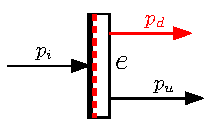
\includegraphics[height=0.13\linewidth]{figs_tikz/sl_bush_e}
	\caption{$H_{\text{bus}}$ icon including energy stock}
	\label{fig:sl_bush_e:bis}
\end{figure}

It was already explained in \ref{sec:hbusinsd} and will serve as the building block for all the other components developed for Power Systems.

\subsubsection{Long Voltage Divider (LVD)}
\begin{figure}
\centering
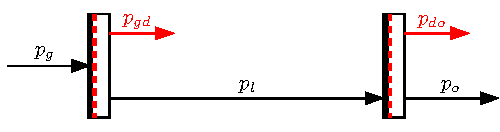
\includegraphics[height=0.13\linewidth]{figs_tikz/slg2bush2_e}
\caption{}
\label{fig:slg2bush2}
\end{figure}
\begin{figure}[h!]
\centering
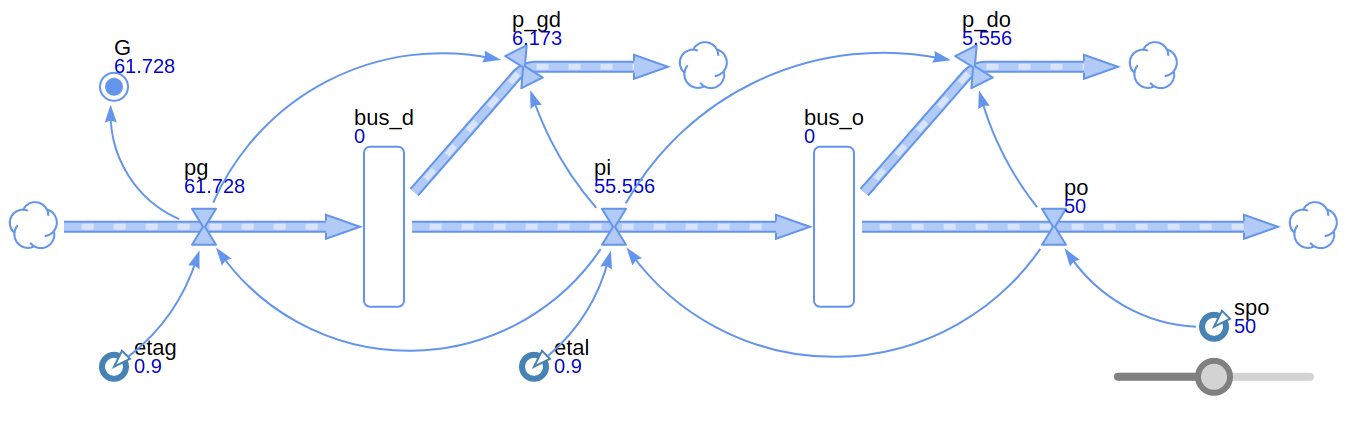
\includegraphics[width=0.65\linewidth]{figs/al_volt_div_long}
\caption{Anylogic implementation of LVD}
%OJO sacada con captura de pantalla de las slides, sería mejor hacerla de nuevo?
\label{fig:alvoltdivlong}
\end{figure}

The SD model is obtained in a straightforward way from its SLD (Figure \ref{fig:slg2bush2}), but conditioning each stock so that  $\sum p =0$, to emulate its physical behavior (a node can't store energy).

For example, for the $o$ bus: $p_l=p_o/\eta_l$
$p_{do} = p_l-p_o$. An alternative way for cases in which discontinuous flows can appear, is to use $\frac{de}{dt} = e_{ref}- a\,e$, with $a=\text{cte}>0$,
$e=\text{bus\_o}$ and $e_{ref}=0$ in the normal case or $e_{ref}=e_{batt}$, to charge a battery.




\subsection{Transmission Lines, Transformers, and Converters}
By leveraging the Hybrid Bus ($H_{bus}$) as the standardized structural vertex, the full array of multi-domain components across a decentralized distribution network can be systematically modeled utilizing pure power-efficiency relationships $(P, \eta)$ \cite{gonzalezdedurana2025novel}. This algebraic syntax neutralizes device-specific coordinates, transforming hardware constraints into scalable graph linkages.


\subsubsection{Transmission lines}

From the perspective of active power-flow dynamics, an electrical conductor or transmission line segment operating in steady state acts as an ideal resistance that dissipates energy to the environment. Consequently, its System Dynamics (SD) graph matches the basic voltage divider structure, where the downstream power vector satisfies $p_j(t) = \eta_{\text{line}} \cdot p_i(t)$, and $\eta_{\text{line}} \in [0, 1]$ encapsulates the line distance and nominal ohmic losses \cite{Nagsarkar2007}.


Transmission lines are necessary to transmit electrical power from energy generators to consumers, which can be located at several distances, from tens of kilometers to a few meters. They can operate in high
\begin{figure}[h]
\centering
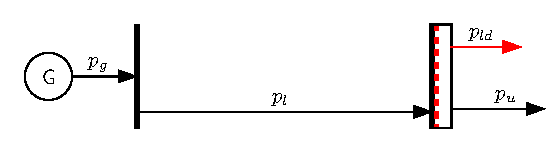
\includegraphics[width=0.45\linewidth]{figs_tikz/sl2transline_e}
\caption{Figure 20: Transmission line}
\label{fig:sl2transline}
\end{figure}
AC three-phasic voltage, typically above 100 kV for long-distance lines, to reduce energy losses and increase efficiency, or in low AC or DC voltage for short-distance distribution lines.

\begin{figure}[h!]
\centering
%\includegraphics[width=0.49\linewidth]{figs/al_m2xhbus}
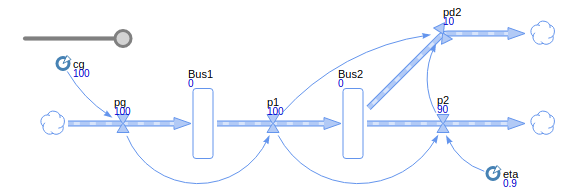
\includegraphics[width=0.6\linewidth]{figs/al_r2xhbus}
\caption{Transmission line modeling and simulation in Anylogic}
\label{fig:alm2xhbus}
\end{figure}

{SD model}.
Essentially, the SD graph for this element is the same as the previous voltage divider because, from the point of view of active power a line behaves like a resistance.


\subsubsection{Electrical Transformers}

An electric transformer is an AC device that transfers the electrical power from an input circuit to another output circuit, both on the same frequency, maybe increasing the voltage $ v_i $ to $ v_o $ , decreasing it, with the corresponding decrease in the electric current $ i_i $ to $ i_o $ or
increasing it, and roughly preserving the power, i.e.
$ p_i = v_i\, i_i \approx v_o i_o = p_o $ .

\begin{figure}[h!]
\centering
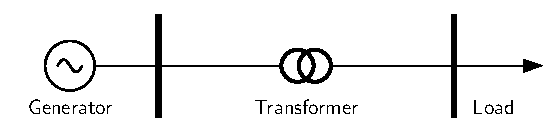
\includegraphics[width=0.52\linewidth]{figs_tikz/sl2transformer}
\caption{Transformer}
\label{fig:transformer}
\end{figure}
Because a small fraction of the associated magnetic flux escapes into the environment as core losses, the device behavior is completely modeled in the power domain by its nominal efficiency index: $\eta_{\text{trans}} = p_{\text{out}}(t) / p_{\text{in}}(t)$, typically exhibiting high coefficients ($\eta \approx 0.99$).

The transformer SD model is very similar to the previous ones, also based on efficiency. This parameter is defined as
\[
\eta = \frac{p_o}{p_i}
\]
that is the rate between their output and input powers.
% Pagina 17
\begin{figure}[h!]
\centering
%\includegraphics[width=0.49\linewidth]{figs/al_m2xhbus}
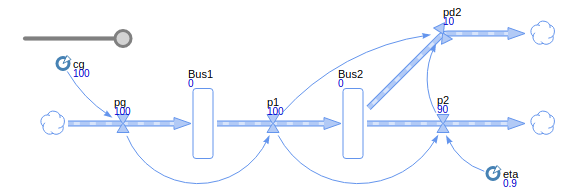
\includegraphics[width=0.6\linewidth]{figs/al_r2xhbus}
\caption{Transformer modeling and simulation in Anylogic}
\label{fig:diagram_al_m2xhbus}
\end{figure}

As it can be seen, the only difference between this model and the previous ones is the efficiency value that was $\eta$ = 0.9 for the voltage divider and line, and $\eta$ = 0.99 for the transformer.


\subsubsection{Electronic AC/DC Converters}

Electronic AC/DC converters are devices that convert a source of alternating current AC to DC, at some specified voltage level. They are widely deployed to interface alternating current grids with continuous distribution structures \cite{rodriguez2026isolated}, being widely used in various applications, including power supplies, electronic devices, and renewable energy systems ~\cite{rodriguez2026isolated}.

Their power-flow behavior is governed by the efficiency operator
\[
\eta = \frac{p_o}{p_i}
\]
where $ p_i $ and $ p_o $ are its input and output powers, respectively, is normally between 80\% to 90\%, although some equipment can achieve higher efficiencies, up to 95\%.

The SD model of one of these pieces of equipment is very similar to that of a transformer, the only difference is that while the transformer convert from AC to AC, this one does from AC to DC.

\begin{figure}[h!]
\centering
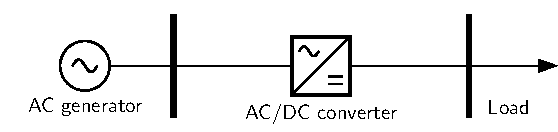
\includegraphics[width=0.48\linewidth]{figs_tikz/sl2acdc}
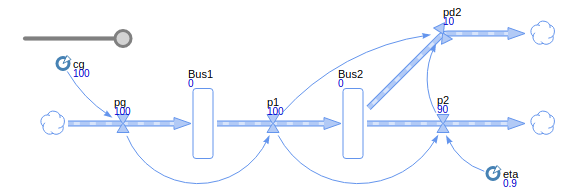
\includegraphics[width=0.48\linewidth]{figs/al_r2xhbus}
\caption{AC/DC SLD and SD Anylogic model}
\label{fig:diagram_al_m2xhbus1}
\end{figure}

%Pagina 18


\subsubsection{Electronic DC/DC Converters}

In renewable-dominated DC architectures, bidirectional DC/DC converters represent the critical control nodes required to manage power flows among heterogeneous assets \cite{energies2025dcdc}.

Electronic DC/DC converters are  devices that convert a source of direct current DC from one voltage level to another (Figure \ref{fig:sl2dcdc} on the left). Its efficiency,
\[
\eta = \frac{p_o}{p_i}
\]
where $ p_i $ and $ p_o $ are its input and output powers, respectively, is usually rather high, ranging from 87\% to 92\% but sometimes they reach exceptionally high values, above 99\%.


\begin{figure}[h!]
\centering
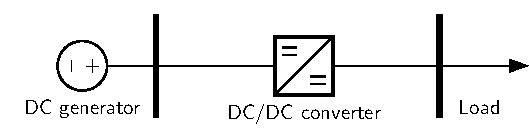
\includegraphics[width=0.48\linewidth]{figs_tikz/sl2dcdc}
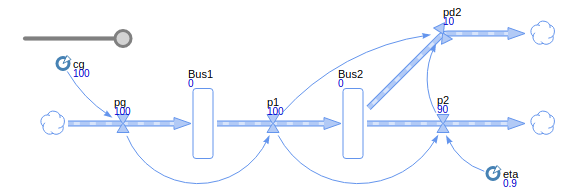
\includegraphics[width=0.48\linewidth]{figs/al_r2xhbus}
\caption{DC/DC SLD and SD Anylogic model}
\label{fig:sl2dcdc}
\end{figure}

Within the architecture of renewable-dominated DC distribution networks, bidirectional DC/DC converters represent the critical operative nodes required to stabilize bus voltage and manage power flows among heterogeneous storage units ~\cite{energies2025dcdc}.

The SD model of one of these pieces of equipment is very similar to that of transformer, the only difference is that while the transformer convert from AC to DC, this one does from DC to DC (Figure \ref{fig:sl2dcdc} on the right).

\subsubsection{Energy storage elements} \label{sec:storage}

Within decentralized networks, energy storage systems (BESS) are essential to mitigate the intermitency of renewable generation \cite{gharbia2026energy}. An SD stock variable $e(t)$ provides an ideal mathematical primitive to model a battery cell, tracking the continuous accumulation of energy through the linear first-order differential equation:
\begin{equation}
        \frac{de(t)}{dt} = p_{\text{charge}}(t) - p_{\text{discharge}}(t)
\end{equation}
where $p_{\text{charge}}$ and $p_{\text{discharge}}$ represent the active input and output power flows governed by the localized charger and battery constraints.

Within the category of decentralized energy networks, energy storage elements—ranging from fast-response electrochemical battery systems to large-scale mechanical and thermal topologies—play a fundamental role as necessary temporal buffers to mitigate the inherent intermittency of variable renewable generation~\cite{gharbia2026energy}.

An SD stock element is an ideal representation for an energy storage element  as Figure \ref{fig:battery} shows, where $ e $ represents the stored energy.


% Pagina19

\begin{figure}[h]
\centering
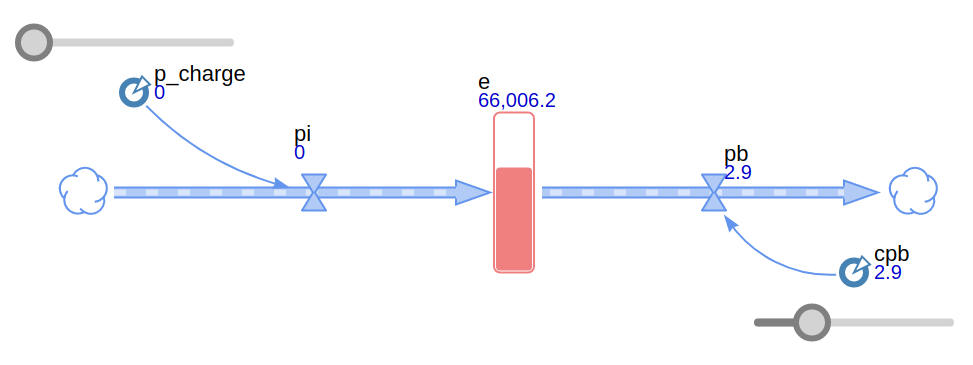
\includegraphics[width=0.49\linewidth]{figs/al_battery_run}
\caption{SD Stock as energy storage element (Anylogic)}
\label{fig:battery}
\end{figure}
% Figure 27:


In this model, energy $e$ is determined by the linear first-order differential equation
\[
\frac{de}{dt} = p_i - p_b
\]
where $ p_i $ and  $ p_b $ are the input and output power flows, respectively.

This model could be adapted to any battery charge or discharge processes working in a simultaneous way in some cases or having independent charge and discharge processes.

Power flows of charge $ p_{\mathrm{charge}} $ and discharge $ p_b$ will depend on the charger device and battery type, respectively, and are modeled using slides in the Figure \ref{fig:battery} model.

%For instance the Long Range battery for Tesla Model S, have a capacity of 100 kWh i.e. 100 × 3, 600, 000 = 360 × 109 J.

%The Tesla Model S power consumption at 100 km/h is approximately 25 kW
%Tiempo = 100 kWh / 25 kW Tiempo = 4 horas, 100 kWh = 360000 kW s
%Tesla Model S vith v= 100 km/h, consumiendo constantemente 25 kW, la batería de 100 kWh le durará aproximadamente 4 horas.



\subsubsection{Interrupters and Circuit Breakers} \label{interr}

Circuit breakers are protection devices designed to cut off power transmission under fault conditions \cite{energies2025circuitbreaker}. Because continuous-time system dynamics platforms lack native mechanisms to open coordinate branches, the operation of an interrupter is abstractly mapped onto the efficiency operator $\eta$. When the circuit breaker is commanded to open, the line topology is severed by driving the link efficiency instantly to zero:
\begin{equation}
        \eta(t) = \begin{cases} \eta_{\text{nominal}} \approx 1.0 & \text{if breaker is closed} \\ 0.0 & \text{if breaker is open} \end{cases}
\end{equation}
    This formulation ensures that the output power drops instantly to zero ($p_{\text{out}} = 0$), forcing the upstream power vector to be absorbed into the loss channel $p_d = p_{\text{in}}$, which successfully replicates the physical interruption behavior without triggering division-by-zero numerical errors in the solver.

Both, interrupters and circuit breakers, are devices designed to cut off the power flowing through one or more power lines. Their differences are on the material they are built, maybe resistant to high temperatures, on the dynamic way they open or close the associated circuit, more or less fast, and on the maximum power they can manage. Within the operational constraints of multi-terminal DC microgrids, interrupters and solid-state circuit breakers represent the critical protection nodes that govern fault isolation ~\cite{energies2025circuitbreaker}.

As no way exists in the SD modeling methods used here to cut a power line, because power and efficiency are the only available elements, some thinking is necessary to try to find a possible way to do, if not the same, something that produces similar effects.

\begin{figure}[h!]
\centering
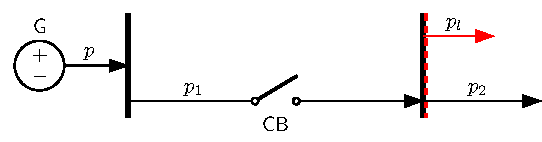
\includegraphics[height=0.13\linewidth]{figs_tikz/sl2interrupt}
\caption{Line interrupter}
\label{fig:sl2interrupt}
\end{figure}
% Figure 28:

Consider the power system shown in Figure \ref{fig:sl2interrupt} where CB denotes Circuit Breaker where $ p_l $ the loss power on the line.

If CB is closed, then, assuming negligible wire resistance, the lost power will be $ p_l \approx 0 $ and then $p_2=p_1$. But if it is open, then the output power $ p_2 $ will be zero so lost power will be $ p_l = p_1 - p_2 = p_1 $. As efficiency is
\[
\eta = \frac{p_2}{p_1}
\]
If CB is closed, it will have a value $\eta \approx 1$ and, if CB is open, it will be $ p_2 = 0 $ so $\eta=0$.

So, in order to model this element, variable $ pd $ should be an input in the model. In this way the $ pd $ value will not be given at start time, but the user will enter it at run time, similar to what occurs in actual interrupters. In this way, the efficiency value can be obtained from $ p_d $:
\[
 \eta = \frac{p_1-p_l}{p_1} = 1- \frac{p_l}{p_1} =
\begin{cases}
 \eta_1 \approx 1\; \text{if CB is closed} \\
0 \quad \text{if CB is open}
\end{cases}
\]
so an indirect way to enter the value of $\eta$, using $ p_l $ as an input, is found.

Note that, in this case the hybrid $H_{\text{bus}}$ does not store energy since $p_l$ is produced by the switch.




\subsubsection{Exogenous actions}

Section \ref{interr} examined the application of System Dynamics (SD) inputs in modeling interrupters. Inputs are a subset of exogenous variables originating externally (typically from user interactions). However, a broader analysis of exogenous variables and their role in system modeling is necessary. In the context of power systems, only the power values $p_1$ and $p_2$ (measured at the left and right of a bus, respectively) can be directly observed, leading to the derivation of line power flow as $p_l=p_1-p_2$.
Smart meters can be strategically deployed along transmission lines-singly, in pairs, or at multiple locations, depending on the length and segmentation of the line. In cases where a line breaker is present, at least two smart meters should be installed to monitor and measure power flow disruptions effectively.

Smart meters, equipped with advanced communication protocols, real-time monitoring capabilities, and integrated sensors, enhance grid security and detect network attacks. Their contributions to cybersecurity in modern power grids can be categorized as follows:
\begin{enumerate}
\item Vulnerability Assessments

Smart meters can conduct proactive vulnerability assessments, identifying potential weaknesses in the network. Monitoring operational parameters helps utilities detect vulnerabilities before malicious actors can exploit them.

\item Anomaly Detection

Leveraging machine learning algorithms and pattern recognition techniques, smart meters can identify irregular behaviors in network traffic. Anomalous deviations in power consumption, voltage fluctuations, or unexpected load variations can indicate potential cyber intrusions or malicious activities.

\item Encryption and Secure Communication

Smart meters employ encryption mechanisms and secure authentication protocols to safeguard data transmission. Encryption ensures end-to-end data integrity, minimizing the risk of unauthorized interception and manipulation of critical grid information.

\item Network Segmentation and Attack Surface Reduction

The architecture of smart meter networks can be designed to operate on segmented and isolated communication infrastructures, reducing the potential attack surface. This segmentation enhances security by limiting attackers' lateral movement within the network, restricting their ability to propagate threats.

\item Intrusion Detection Systems (IDS)

Some smart meters have intrusion detection capabilities, enabling them to recognize and alert utilities about potential security incidents in real-time. These intrusion detection systems (IDS) analyze network traffic patterns and trigger alerts when deviations from normal behavior occur.

\item Proactive Monitoring and Threat Mitigation

Continuous monitoring, regular software updates, security patches, and robust vulnerability management strategies contribute to maintaining the integrity and resilience of smart meter infrastructures. By actively addressing emerging cybersecurity threats, utilities can enhance the long-term reliability and security of the smart grid.

By integrating these security-enhancing features, smart meters play a pivotal role in fortifying modern power grid infrastructures. Their ability to detect, prevent, and mitigate cyber threats enhances operational resilience and energy reliability. The increasing deployment of smart meters underscores their significance in transitioning toward secure, intelligent, and adaptive energy networks.
\end{enumerate}

By integrating these security-enhancing features, smart meters play a pivotal role in fortifying modern power grid infrastructures. Their ability to detect, prevent, and mitigate cyber threats enhances operational resilience and energy reliability. The increasing deployment of smart meters underscores their significance in transitioning toward secure, intelligent, and adaptive energy networks.


%
%Smart meters, equipped with advanced communication protocols and sensors, play
%a crucial role in identifying and detecting network attacks. Here are some ways they contribute:
%
%Vulnerability assessments: Smart meters can be used to conduct vulnerability assessments, helping to identify potential weaknesses in the network and allowing utilities to address them before attackers exploit them.
%
%Anomaly detection: Smart meters’ advanced sensors and algorithms can detect unusual patterns or behavior in network traffic, indicating potential malicious activity. Encryption and secure communication: Smart meters use encryption to protect data transmission, making it more difficult for attackers to intercept and manipulate sensitive information.
%
%Segmented networks: Smart meters can be designed to operate on isolated networks, reducing the attack surface and making it harder for attackers to move laterally within the system.
%
%Intrusion detection systems (IDS): Some smart meters are equipped with IDS capabilities, allowing them to detect and alert utilities to potential security incidents in real-time.
%
%Proactive monitoring: Regular software updates, patching, and vulnerability management ensure that smart meters remain secure and resilient against emerging threats.
%
%By incorporating these features, smart meters can help utilities and grid operators detect and respond to network attacks more effectively, ultimately enhancing the overall security and reliability of the smart grid.


\section{Practical Examples}
\label{sec:practical_cases}


To illustrate the applicability of the methodology in modeling electrical power systems, this section presents two practical case studies: a CubeSat electrical power system (EPS) and a microgrid consisting of four residential units powered by renewable energy sources. The first example focuses on the CubeSat EPS, where SD is used to model the energy generation, storage, and consumption dynamics of a small satellite operating in orbit. This model accounts for the periodic charging of batteries via solar arrays during sunlight exposure and subsequent power distribution to onboard systems during eclipse periods. The second example explores the operation of a small-scale microgrid, integrating solar panels and a wind turbine to supply power to four houses. The SD approach allows for a detailed analysis of energy generation, load balancing, and dynamic power distribution, considering variations in renewable energy availability and household demand. These case studies demonstrate the flexibility and effectiveness of this methodology in modeling energy networks, providing insights into the performance, adaptability, and resilience of modern power systems.


But before, a basic circuit that will be a common part for any other microgrid models, is described and modeled.


\subsection{Basic circuit for a microgrid}
To evaluate the scalability of the Power Dynamics framework, a benchmark microgrid circuit that extends the long voltage divider topology is defined. As illustrated in Figure~\ref{fig:mgrid3v4r}, this system comprises three parallel voltage generators ($v_1, v_2, v_3$) with internal resistances ($r_1, r_2, r_3$) connected to a generation bus (node $d$), four parallel loads ($R_1, R_2, R_3, R_4$) connected to a distribution bus (node $o$), and a transmission line with resistance $r_d$ linking both vertices.

The Single-Line Diagram (SLD) maps this topology into a pure power-efficiency graph where generators $G_1, G_2, G_3$ inject power flows $p_{g1}, p_{g2}, p_{g3}$, and loads consume $p_{l1}, p_{l2}, p_{l3}, p_{l4}$. In the AnyLogic simulation environment, the stock elements are conditioned to satisfy $\sum P = 0$. Four manual sliders are utilized to dynamically demand load powers, while two sliders govern generation injection. Generator $G_3$ is configured as a Slack bus, automatically absorbing or injecting the remaining balance required to preserve the continuous network equilibrium.



\begin{figure}[h!]
\centering
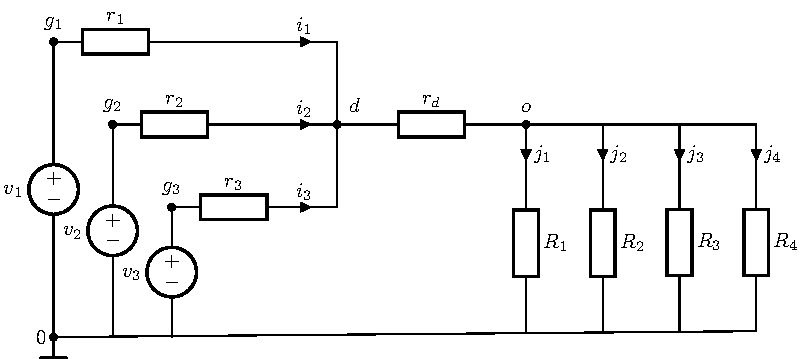
\includegraphics[width=0.7\linewidth]{figs_tikz/mgrid3v4r}
\caption{Basic circuit for a microgrid}
\label{fig:mgrid3v4r}
\end{figure}

Note that this circuit follows from the long voltage divider by replacing the  voltage generator by three ones and the load resistor by four ones.


\subsection*{SLD diagram and SD model}

The SLD of this circuit can be easily obtained from the SLD
corresponding to the LVD, by putting three generators $G_1, G_2, G_3$ in parallel instead of $G$, which inject the power flows $p_{g1}, p_{g2}, p_{g3}$, and four load resistors in parallel
$R_1, R_2, R_3, R_4 $ instead of $R$, which consume the powers $p_{l1}, p_{l2}, p_{l3}, p_{l4}$.

\begin{figure}[h]
\centering
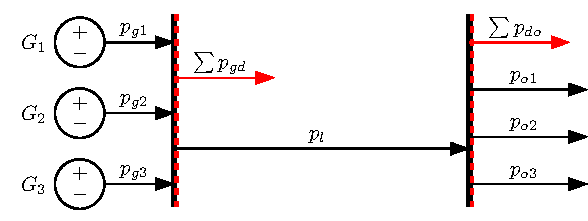
\includegraphics[width=0.5\linewidth]{figs_tikz/mgrid3v4r_sld}
\caption{SLD for the basic microgrid circuit}
\label{fig:mgrid3v4rsld}
\end{figure}



\subsubsection*{SD Model in Anylogic}
It can be easily obtained from the SD diagram of the
VD, keeping the variables $i$ and $v_o $ of that
diagram (here $v = v_o $).
\begin{figure}[h]
\centering
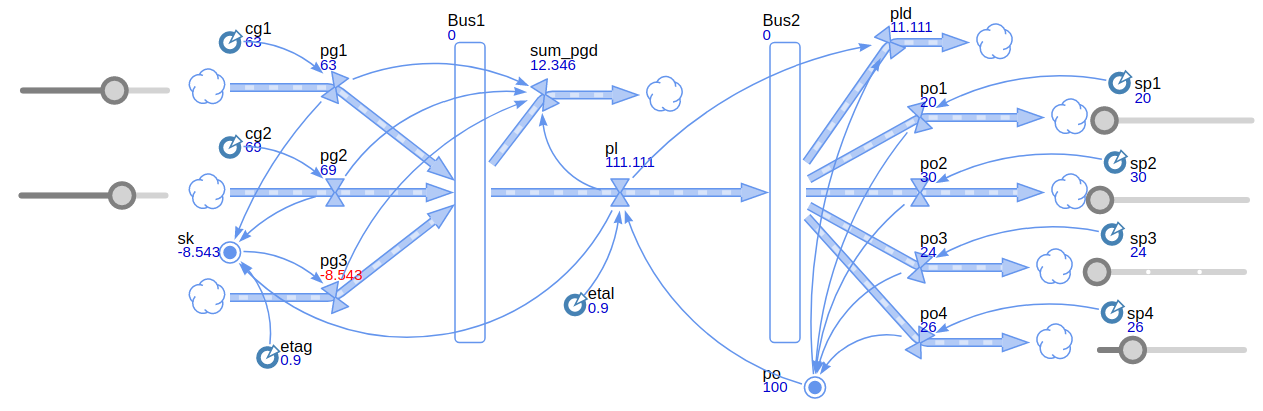
\includegraphics[width=\linewidth]{figs/al_mgrid3v4r}
\caption{AL model for the basic microgrid circuit}
\label{fig:almgrid3v4r}
\end{figure}

As in the LVD, the AL model gets from its SLD, but
conditioning each stock in SD so that $\Sigma_p = 0 $:\\
Bus2: $p_o = p_{o1} + p_{o2} + p_{o3} + p_{o4}, p_l = p_o /\eta1 p_{ld} = p_l - p_o$\\
Bus1: $s_k = p_l /\eta_2 - p_{g1} - p_{g2}, \text{sum\_pgd} = p_{g1}+p_{g2}+p_{g3}-p_l$\\
4 sliders are used to demand powers $p_{o1}, p_{o2}, p_{o3}, p_{o4}$\\
2 sliders are used to inject powers $p_{g1}$ y $p_{g2}$\\
Generator
$G_3$ is type Slack: it injects/sink the necessary power $ p_{g3} $  to fulfill $\Sigma p =0$.


\subsection{Space infrastructure simulation: cubeSat EPS}
To validate the multi-domain scalability of the developed $(P, \eta)$ abstract syntax, the first case study implements the complete Electrical Power System (EPS) of a 1U miniaturized satellite (CubeSat) operating in low Earth orbit. Traditional satellite power bus simulations rely heavily on hardware-specific orbital models that solve high-order semiconductor switching equations, introducing severe computational penalties during long-term mission horizon planning.

The CubeSat architecture integrates power generation (solar arrays), energy storage (batteries), and a power management layer that handles distribution to the payload, communications, and attitude control systems. The operational dynamics are characterized by cyclic transitions between sunlit generation windows and eclipse periods. During sunlit regimes, the generation flow $p_{\text{gen}}(t)$ represents the active conversion profile of the deployed solar panels. This structural input charges the localized battery stock variable $e(t)$, which governs the energy storage capacity according to the linear balance equation $\dot{e}(t) = \sum p_{\text{sun}} - p_{\text{discharge}}$. Conversely, during eclipse crossings, the input flow drops instantly to zero ($p_{\text{gen}} = 0$), forcing the battery stock to become the sole operative source. The power management layer applies a rule-based priority routing scheme, ensuring that critical subsystem flows (e.g., communications and attitude control) are preserved before allocating energy to secondary payloads, successfully mapping the complex satellite mission space within a smooth System Dynamics platform.


In the System Dynamics (SD) framework, these points are modeled as stock variables that track active energy states without handling transistor-level semiconductor equations. The simulation runs cycles of sunlight and eclipse: during sunlit windows, the input flow from the solar panels charges the battery stock according to cell efficiency and orientation metrics. Conversely, eclipse transitions drive the generation flow to zero, forcing the battery to discharge aggressively. The control logic applies a rule-based priority routing scheme, ensuring that critical communication links receive power before secondary payloads. This demonstrates the modular flexibility of the $(P, \eta)$ syntax to capture cross-domain satellite lifecycles under extreme operational profiles.


\begin{figure}[h!]
    \centering
    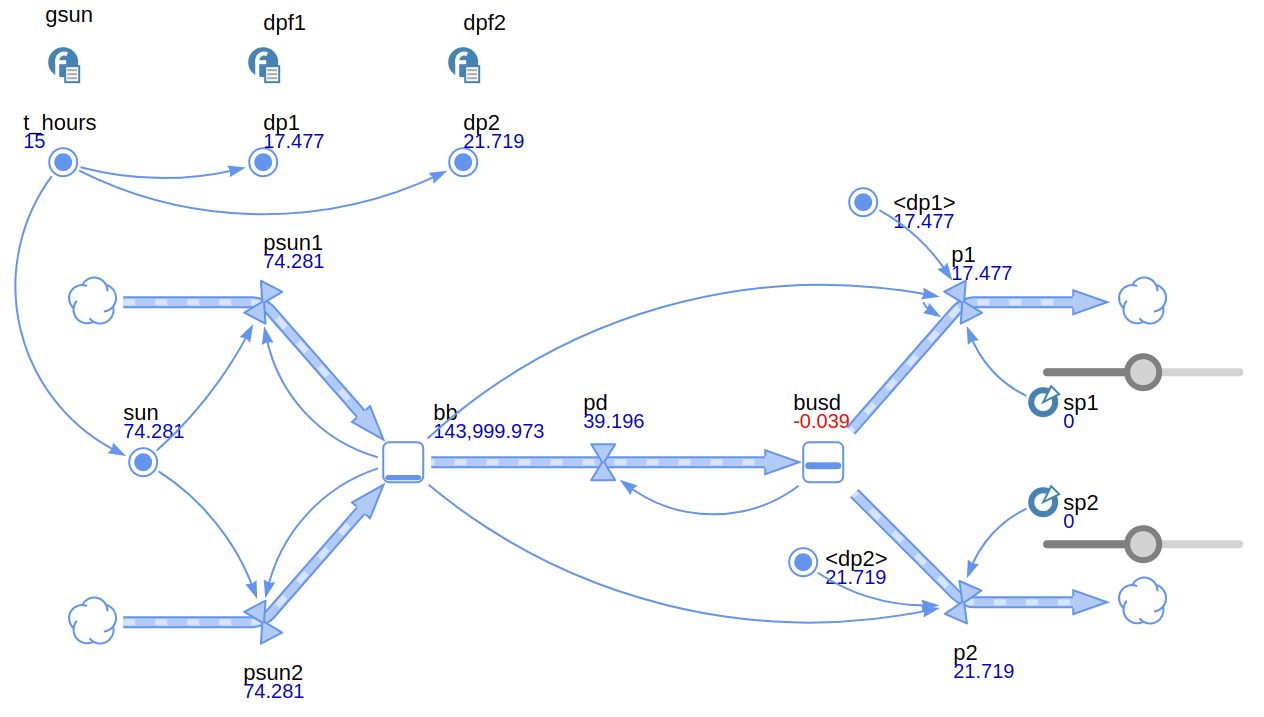
\includegraphics[width=0.7\linewidth]{figs/al_cubesat}
    \caption{Power-dynamics graph of the CubeSat EPS inside AnyLogic.}
    \label{fig:al_cubesat_detailed}
\end{figure}



A CubeSat is a type of miniaturized satellite used for space research, typically built in a standardized cubic form factor. The most common size is a 1U CubeSat, which measures 10x10x10 cm and weighs about 1.33 kg, though larger configurations like 2U, 3U, or 6U are also used. CubeSats are often deployed in low Earth orbit for purposes such as Earth observation, technology demonstration, scientific experiments, and educational projects. Their compact size and relatively low cost make them accessible to universities, research institutions, and private companies.

A 1U CubeSat (10x10x10 cm) typically has the following main features, though specifics can vary depending on the mission and design:
\begin{itemize}
\item  4 to 6 solar panels, generating around 2-4 watts each

\item typically 1-2 battery packs with capacity from 10-30 Wh

\item Total power consumption from 2-10 W
\end{itemize}
\textbf{A CubeSat Electrical Power System (EPS)} is a critical subsystem responsible for generating, storing, distributing, and managing electrical power for the satellite.


Steps to Model the EPS of a CubeSat Using System Dynamics
\begin{enumerate}
\item  Define System Boundaries and Components:
\begin{itemize}
\item Subsystems: CubeSat's EPS consists of power generation (solar arrays), energy storage (batteries), and power management (distribution to payload, communications, and attitude control systems).
\item  Power Generation: Solar arrays generate power during sunlit periods, which is stored in batteries for use during eclipse periods.
\item  Energy Storage: Batteries store the excess energy generated by solar arrays and discharge energy to the CubeSat systems during power demand peaks or eclipse periods.
\end{itemize}
\item  Modeling Power Nodes as Stock Elements:
\begin{itemize}
\item  In SD, power at different points in the system (e.g., generated by solar panels, stored in batteries, and consumed by different subsystems) can be represented as stocks. These stocks represent the accumulation of power in different parts of the CubeSat.
\item  For instance, one stock could represent the energy stored in the batteries, while another stock could represent the power available for immediate consumption by the satellite's systems.
\end{itemize}
\item  Define Power Flows Between Components:
\begin{itemize}
\item  Solar Power Flow: A flow from the solar panels to the battery stock during periods of sunlight. The flow rate is determined by the solar panel's efficiency, orientation to the sun, and environmental factors.
\item  Discharge Flow: A flow from the battery to the satellite subsystems during periods of power demand, such as when the CubeSat is in eclipse or during high-power activities like image capturing and data transmission.
\item  Energy Balance: As with the paper’s DC systems model, an energy balance equation ensures that energy generated during sunlight periods meets the demands during eclipse periods.
\end{itemize}
\item  Implement Control Logic Using SD Flows:
\begin{itemize}
\item  Regulation: Use SD flow elements to model the behavior of power regulation components like DC-DC converters, ensuring that the right voltage and current are supplied to different subsystems.
\item  Power Prioritization: Certain flows can represent the priority of energy usage, ensuring that critical systems like communications or attitude control receive power before non-essential systems.
\end{itemize}
\item  Simulation of Energy Dynamics:
\begin{itemize}
\item  Orbit Cycles: The CubeSat operates in cycles of sunlight and eclipse, which can be modeled by varying the input flow of energy into the system (solar panel input) based on the CubeSat's orbital position. Eclipse times lead to increased discharge from the battery stock.
\item  Energy Dissipation: Include losses due to inefficiencies in power generation, storage, and transmission as part of the power flows.
\item  Test Scenarios for Different Operating Conditions:
\end{itemize}
\begin{itemize}
\item  High-Demand Scenarios: Model scenarios where the CubeSat is executing high-power tasks like imaging or downlinking large amounts of data. In this scenario, the discharge rate from the batteries will increase, and the model can simulate how the battery stock depletes and recharges over time.
\item  Contingency Operations: In the event of an anomaly or low-battery situation, the SD model can simulate a ``safe mode'' where only essential systems receive power, reducing the load and allowing the batteries to recharge faster.
\end{itemize}
\item  Refinement and Optimization:
\begin{itemize}
\item  Parameter Tuning: Use SD to run different simulations with varying solar panel efficiencies, battery capacities, and orbital parameters to determine the optimal EPS design that ensures continuous power availability.
\item  Energy Balance: Using System Dynamics ensures that energy is conserved within the CubeSat system, and any imbalance in power generation or consumption over time can be identified and mitigated.
\end{itemize}
\end{enumerate}

Benefits of Using System Dynamics for EPS Modeling in CubeSats
This is a comprehensive framework for modeling energy generation, storage, and consumption within the CubeSat's Electrical Power System (EPS). By ensuring that energy flows are consistent with the laws of conservation, SD enables a precise understanding of power dynamics throughout the satellite’s operational lifecycle. This approach facilitates the identification of potential energy deficits, storage limitations, and optimization opportunities, contributing to the efficient management of onboard power resources.

The modular nature of SD modeling allows for seamless scalability, enabling the extension of the CubeSat EPS model to more complex satellite configurations. Additional power subsystems, such as secondary energy storage, dynamic load balancing mechanisms, or alternative power generation sources (e.g., radioisotope thermoelectric generators for deep-space missions), can be incorporated without requiring significant model restructuring. Furthermore, SD models can be expanded to simulate multi-satellite constellations where power sharing, inter-satellite energy transfers, or collaborative power management strategies need to be considered.
SD's flexibility enables CubeSat EPS simulations under various operational scenarios, including different orbital altitudes, solar panel degradation, battery aging effects, and varying eclipse durations. This adaptability supports robust pre-deployment testing by allowing engineers to explore worst-case conditions, emergency power reallocations, and optimal energy dispatching strategies.

Beyond electrical power systems, SD modeling can be integrated with other non-electrical subsystems, such as reasoning control systems that facilitate qualitative decision-making. For instance, a high-level control layer can be added to the CubeSat model, incorporating AI-driven or rule-based decision-making frameworks to dynamically prioritize power allocation for critical subsystems. Such a system could determine when to activate or deactivate non-essential payloads, switch between primary and backup power sources, or engage emergency power-saving modes based on mission objectives and environmental conditions.

The framework supports the integration of cross-domain system models, allowing the CubeSat EPS to be connected with thermal regulation models, attitude control systems, and communication subsystems. By linking these domains, a fully dynamic and interactive simulation environment can be created, where power management strategies respond to thermal constraints, data transmission requirements, or external disturbances.


\subsubsection{Microgrid for Four Residential Units Powered by Renewable Energy Sources}

The second application analyzes a localized, direct current (DC) microgrid designed to supply power to four independent residential units.

This example analyzes the dynamic modeling of a small-scale direct current (DC) microgrid, integrating localized solar panels and a wind turbine to supply power to four distinct residential houses, as depicted in the topological configuration of Figure~\ref{fig:alpf4house1}. The proposed System Dynamics (SD) approach allows for a detailed operational analysis of energy generation, load balancing, and dynamic power distribution, explicitly considering variations in renewable energy availability and household demand profile combinations.

\begin{figure}[h]
\centering
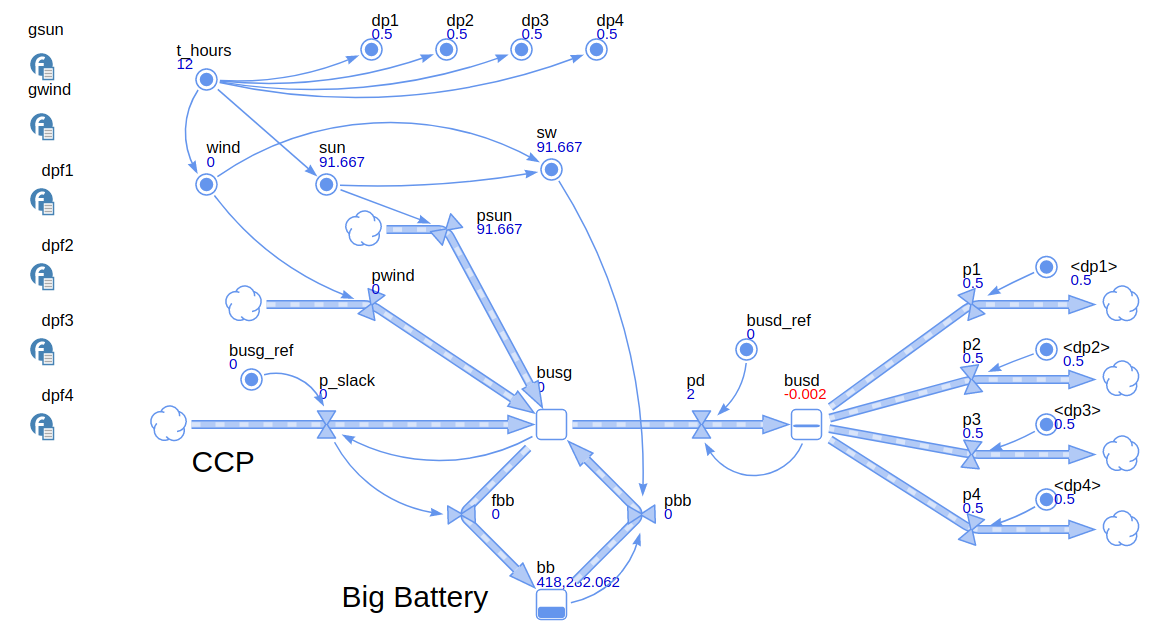
\includegraphics[width=\linewidth]{figs/al_pf4house}
\caption{AL model of a Microgrid for four households.}
\label{fig:alpf4house1}
\end{figure}


Within this AnyLogic execution environment, the \textsf{wind} and \textsf{sun} renewable generators are governed by empirical table-functions denoted as \textsf{gsun} and \textsf{gwind}, respectively. The household demand powers $p_1, p_2, p_3, p_4$ are dynamically driven by variables $d_{p1}, d_{p2}, d_{p3}, d_{p4}$, which are anchored to their respective localized consumption profiles \textsf{dpf1}, \textsf{dpf2}, \textsf{dpf3}, and \textsf{dpf4}. The aggregate magnitude of this power is absorbed directly from \textsf{busd}, which subsequently demands the net power flow \textsf{pd} through a continuous feedback loop. Concurrently, the external supply network injects through the slack channel \textsf{p\_slack} the exact necessary power flow required to maintain a strict zero energy state at \textsf{busg} via localized proportional feedback.


To balance this network against high renewable volatility, a storage system named \textsf{Big Battery} is deployed to accumulate energy whenever localized generation overflows household consumption. The simulation environment enforces the following operational constraints:
\begin{itemize}
    \item The storage device is modeled as an initially fully charged battery with a capacity of $40\,\text{Wh}$ ($144,000\,\text{J}$).
    \item The battery is charged by the incoming power flows \textsf{psun} and \textsf{pwind} until it reaches its maximum nominal saturation ceiling. Conversely, it is discharged by the net power demand flow \textsf{pd}.
    \item The power vector \textsf{pd} is demanded to the distribution bus \textsf{busd} provided that the residual battery energy satisfies the threshold condition $bb > 10,000\,\text{J}$.
    \item Specifically, individual load power $p_1$ is demanded to \textsf{busd} under the condition that the battery internal energy status satisfies $bb > 10,000\,\text{J}$.
    \item The structural power flow $p_d$ corresponding to loads $p_1, p_2, p_3, p_4$ is requested through an active feedback loop linked directly to the battery state variable \textsf{bb}.
    \item To simulate external perturbations or micro-grid human interventions, each manual interface slider can add a dynamic power variance bounded between $-10\,\text{W}$ and $+10\,\text{W}$.
\end{itemize}

From an epistemological standpoint, these case studies demonstrate the significant flexibility and effectiveness of the ``Power Dynamics'' methodology in modeling energy networks. By utilizing the Hybrid Bus ($H_{\text{bus}}$) syntax to neutralize hardware-dependent circuit coordinates into pure power-efficiency relations, the multi-node simulation avoids the matrix inversion loops that typically slow down traditional solvers.

Furthermore, this decentralized arrangement provides critical insights into the performance, adaptability, and resilience of modern power systems. As shown by the slider-induced perturbations and the abrupt $bb$ threshold transitions, the abstract model is uniquely suited for characterizing complex environments subject to rapid discrete events, physical contingencies, or cyber-attacks (such as False Data Injection or Denial-of-Service vectors). The power-oriented syntax allows discrete-event simulators to overlay security disruptions seamlessly, tracking system-level energy deficits and wide-area resilience while completely avoiding numerical stiffness or convergence failures during severe sequence transitions. This convergence of laboratory-level telemetry and abstract graph computation successfully seals the \textit{Systematic Synthetic Identity} of the model, transforming the formal reduction into a necessary interpretation for contemporary engineering praxis.




\subsection{Methodological capacity demonstration.}
 \label{sec:methodological_capacity}

The operational execution of the decentralized CubeSat Electrical Power System (EPS) and the four-household residential DC microgrid serves as a comprehensive, multi-scenario demonstration of the developed framework's methodological capacity. These heterogeneous implementations validate that the abstract
$(P,\eta)$ syntax is not a restrictive linear approximation, but a highly adaptive system language capable of modeling dynamic systems across diverse technological boundaries. By embedding local circuit constraints into the autonomous, first-order immanent architecture of the Hybrid Bus
($H_{bus}$), the modeling workflow achieves three significant goals: first, it filters out the high-frequency electromagnetic noise that typically triggers numerical stiffness in traditional $(V,I,R)$ DAE solvers; second, it guarantees robust global tractability during severe discrete events; and third, it provides a mathematically rigorous, device-independent platform for wide-area energy management. Ultimately, this operational demonstration bridges the historical gap between hardware-level hyperrealism and formal mathematical reductionism, successfully cementing the categorical closure of Pseudolinear Power Systems as an objective, scalable tool for modeling the smart grid and cyber-physical security issues.


\subsubsection{Operational advantages of the $(P, \eta)$ abstraction}
The first-order abstract model based on power variables and efficiency operators $(P, \eta)$ outperforms the traditional second-order circuit representation governed by voltage, current, and resistance $(V, I, R)$ when interacting with discrete-event simulators or hybrid automata \cite{gonzalezdedurana2025novel, en19020304}. This superiority is grounded on specific technical and gnoseological structural advantages detailed below:

\begin{enumerate}
    \item \textbf{Elimination of numerical stiffness and convergence failures:}
    In a standard $(V, I, R)$ configuration, the transmission lines and connections include physical lumped parameters such as loop inductances ($L$) and filter capacitances ($C$). When a discrete event occurs---such as the abrupt disconnection of a load, the isolation of a line segment by a circuit breaker, or a Denial-of-Service (DoS) cyber-attack that disables an inverter---the system variables force a state transition in zero time ($\Delta t \to 0$) \cite{moutevelis2024taxonomy, pr13092969}.
    \begin{itemize}
        \item Within the $(V, I, R)$ framework: this instantaneous transition forces the differential terms (such as $L \frac{di}{dt}$ and $C \frac{dv}{dt}$) to mathematically approach infinity. Numerically, the continuous integration engine faces severe numerical stiffness. The differential-algebraic equation (DAE) solver is forced to reduce its time step to fractions of a nanosecond or, under severe discontinuities, aborts the execution due to convergence failures within the Jacobian matrix \cite{en19020304, moutevelis2024taxonomy}.
        \item Within the $(P, \eta)$ framework: by reducing the system to a clean first-order response and absorbing the fast electromagnetic dynamics inside the efficiency operator $\eta$ (neutralizing the reactive variables at the origin, as demonstrated in Script 7), the continuous transient profiles remain smooth and free of parasitic oscillations \cite{en17143468, biom11020343}. The discrete-event simulator can jump sequentially from one timestamp contingency to another without handling mathematical infinities or stalling inside microsecond-level physical transients.
    \end{itemize}

    \item \textbf{Direct algebraic handling:}
    Contingencies involving the removal of network components or structural topology reconfigurations alter the circuit admittance matrices instantly.
    \begin{itemize}
        \item Within the $(V, I, R)$ framework: if a load resistance $R_2$ is disconnected, resulting in an open circuit where $R \to \infty$, the standard mesh or nodal equations collapse due to mathematical indeterminacies such as $1/R \to 0$ or $R \to \infty$. The simulation engine must halt the continuous execution, reconfigure the sparse matrix topology, and recalculate the initial boundary states from scratch.
        \item Within the $(P, \eta)$ framework: the interconnections are modeled as purely multiplicative and algebraic relations, matching the associative properties of the category $\mathcal{PD}$ ($\eta_{ik} = \eta_{jk} \cdot \eta_{ij}$). Removing a specific line or component reduces simply to commuting the link efficiency operator to zero ($\eta_{ij} = 0$) or deactivating the corresponding power flow $P$. The dimension of the global state space remains invariant, enabling the simulator to execute rapid contingency sequences in DC microgrids without rewriting the system matrix equations \cite{gonzalezdedurana2025novel}.
    \end{itemize}

    \item Native coherence with cybersecurity and digital logic layers:
    modern cyber-physical threats, such as False Data Injection (FDI) attacks, alongside the corrective actions executed by Energy Management Systems (EMS), operate discretely within the communication and digital power layers rather than the analog voltage or current domains \cite{pr13092969, sys12040109}.
    \begin{itemize}
        \item Impact mapping: maliciously altering an inverter power reference or blocking a battery control signal maps directly onto the abstract power graph. It changes the demanded power flow ($P$) or modifies the perceived efficiency index ($\eta$) of the hybrid bus.
        \item Unified Interface Architecture: the $(P, \eta)$ model provides a single native interface where the cyber-attack vector and the physical grid response share the same algebraic syntax. Conversely, evaluating the macroscopic impact of the same cyber-attack within a traditional $(V, I, R)$ model requires translating digital commands into transistor-level gate signals and solving the high-order RLC dynamics across the entire network. This hardware-level modeling quickly becomes computationally intractable for wide-area resilience assessments \cite{moutevelis2024taxonomy, pr13092969, sys12040109, appl14221111}.
    \end{itemize}
\end{enumerate}



% =====================================================================
% SECTION 6: FUTURE PLANS AND MATHEMATICAL FORMALIZATION
% =====================================================================
\section{Future Plans}
\label{sec:future_plans}\label{sec:future}

The aim of this paper is to inspire future research to explore broader formal mathematical formulations for the abstract modeling introduced here and extend the methodology to alternating current networks. Some possible topics for such initiatives are outlined below.


\subsection{Formalization Within Category Theory}
\label{sec:formalcath}

A prominent avenue for future research consists in evolving the mathematical foundation of the $H_{bus}$ framework from traditional Set Theory to Category Theory \cite{maclane1998categories}. This choice is not arbitrary; it aligns with the epistemological foundations of PM Categorial Closure. While Set Theory focuses on static membership, Categorial Closure conceptualizes sciences as dynamic, operatordriven fields defined by transformations and synthetic identities among terms.  Gustavo Bueno was likely aware of Russell's paradox, the antinomies of Cantor's set theory, and the limitations of Hilbert's formalist program in light of Gödel's theorems \cite{godel1931}. Indeed, that famous ``foundational crisis'' in mathematics during the early 20th century is one of the historical pillars Bueno used to justify and shape his own gnoseological theory of Categorial Closure.


Category Theory provides the precise mathematical language required to rigorously model the operational closure and gnoseological mapping as established in the Section \ref{sec:pseudolinear}. This categorical architecture naturally satisfies the identity axiom ($\eta_{ii} = 1$) and the associative composition of morphisms ($\eta_{ik} = \eta_{jk} \cdot \eta_{ij}$) across cascading segments. The topological reduction will be mathematically formalized as a covariant functor $\mathscr{F}$ mapping hardware-level differential equations into power-graph invariants, guaranteeing structural consistency for radial systems.

We define the category $\mathcal{PD}$ (Power Dynamics Category) for decentralized direct current energy systems in steady-state operation as follows:
\begin{itemize}
    \item \textbf{Objects ($\mathrm{Ob}(\mathcal{PD})$):} The objects represent the nodes or abstract vertices of the network, implemented as Hybrid Buses ($H_{bus}$) enforcing instantaneous energy balance.
    \item \textbf{Morphisms ($\mathrm{Hom}(B_i, B_j)$):} The morphisms represent the transmission lines or converters ($l_{ij}$) linking the vertices. A morphism $f: B_i \to B_j$ is defined strictly by the efficiency operator $\eta_{ij} \in [0, 1]$, such that:
    \begin{equation}
        P_j = \eta_{ij} \cdot P_i
    \end{equation}
\end{itemize}




The power-efficiency formulations can be modeled within the framework of Category Theory to verify their structural consistency. By treating network configurations as algebraic structures, direct current (DC) power networks constitute a consistent category, can be proved. Category Theory shifts the foundational focus from objects to the arrows that relate them. This framework inherently mirrors the principles of PM Categorial Closure, where sciences are defined by transformations and synthetic identities rather than static membership.


% =====================================================================
% REVISED CATEGORY THEORY FUNCTOR NOTATION (SECTION 5.1 CLOSURE)
% =====================================================================
The category $\mathcal{PD}$ satisfies the standard algebraic axioms: every bus possesses an identity morphism $\mathrm{id}_{B_i}$ with ideal efficiency $\eta_{ii} = 1.0$, and the composition of morphisms across cascading segments is associative ($\eta_{ik} = \eta_{jk} \cdot \eta_{ij}$), which mathematically guarantees the scalability of the method for radial distribution topologies. The translation from continuous physical layer coordinates ($M_1$) to the abstract domain ($M_3$) constitutes a covariant functor $\mathscr{F} : \mathscr{Elec} \to \mathcal{SD}$ that maps hardware-level differential equations into power-graph invariants, neutralizing hardware-dependent axes.


 \subsubsection*{SLDs as the basis for formalization}
Single-line diagrams (SLDs) describe power networks by preserving circuit topology. A bijective correspondence exists between the physical nodes of an electrical network and the buses of an SLD, creating a direct mapping between physical components and their symbolic representations.

Our framework focuses on distribution networks. Due to their radial structures, these networks can be formulated as an interconnected system of $N$ second-order lines, resulting in a global system of order $2N$ suitable for dominant-pole reduction.

The physical space ($M_1$) connects to the abstract domain ($M_3$), mapping the RLC circuit directly onto the idealized hybrid bus (\textit{Hbus}):
\begin{equation*}
\begin{aligned}
\mathcal{M} : M_1 &\to M_3 \\
\text{RLC Circuit} &\mapsto H_{\text{bus}}
\end{aligned}
\end{equation*}

This mathematical reduction is expressed via a reduction functor, $\mathcal{R}$, that establishes a structural correspondence from the Category of Power Systems (${PowSys}$) to the Category of Pseudolinear Power Systems ($PsLinPowSys$):
\begin{equation*}
\begin{aligned}
\mathcal{R} : \mathrm{PowSys} &\to \mathrm{PsLinPowSys}
\end{aligned}
\end{equation*}



\subsubsection*{The Power Dynamics Category: objects and morphisms}
We define the category $\mathcal{PD}$ (Power Dynamics Category) for decentralized energy systems in steady-state operation:
\begin{itemize}
    \item {Objects ($\mathrm{Ob}(\mathcal{PD})$):} The objects represent the nodes or abstract buses of the power grid, implemented as Hybrid Buses ($H_{\text{bus}}$). Each object $B_i$ is characterized by its power boundaries and its role in instantaneous energy balance.
    \item {Morphisms ($\mathrm{Hom}(B_i, B_j)$):} The morphisms represent the transmission lines or converters ($l_{ij}$) between buses. A morphism $f: B_i \to B_j$ is defined by the efficiency operator $\eta_{ij} \in [0, 1]$, such that:
    \begin{equation}
        P_j = \eta_{ij} \cdot P_i
    \end{equation}
\end{itemize}

\subsubsection*{Axiomatic Closure and Functorial Mapping}
The category $\mathcal{PD}$ satisfies the standard algebraic axioms:
\begin{enumerate}
    \item {Identity Morphism:} For every bus $B_i$, an identity morphism $\mathrm{id}_{B_i}: B_i \to B_i$ exists with ideal efficiency $\eta_{ii} = 1$.
    \item {Composition of Morphisms:} For two cascading segments $f: B_i \to B_j$ (efficiency $\eta_{ij}$) and $g: B_j \to B_k$ (efficiency $\eta_{jk}$), their composition $(g \circ f): B_i \to B_k$ satisfies:
    \begin{equation}
        \eta_{ik} = \eta_{jk} \cdot \eta_{ij}
    \end{equation}
    This composition rule is associative, which ensures the scalability of the method for radial topologies.
\end{enumerate}

The translation from circuit variables ($V, I, R$) to System Dynamics parameters (Stocks and Flows) is modeled as a covariant functor $\mathscr{F}: \mathscr{Elec} \to \mathcal{SD}$. This functor maps the mesh equations into power-graph invariants, neutralizing hardware-dependent coordinates.



\subsection{Future Research Directions in Cybersecurity}
The simulation of both the satellite subsystem and the multi-household residential microgrid demonstrates the significant operational advantages of the $(P, \eta)$ abstraction layer over traditional circuit-level architectures governed by voltage, current, and resistance $(V, I, R)$ \cite{alsbua2026artificial}. When the microgrid model is subjected to severe discrete disruptions—such as manual slider-induced load variations ($\pm 10\,\text{W}$), abrupt circuit breaker failures, or malicious False Data Injection (FDI) cyber-attacks targeting the smart meters—the mathematical framework preserves absolute structural tractability \cite{mu2026data}.

Building upon these findings, future work will leverage this structural tractability to investigate complex wide-area grid vulnerabilities. While traditional circuit models suffer from convergence failures and severe step-size reductions due to derivative spikes ($L \frac{di}{dt}$, $C \frac{dv}{dt}$) during switching changes \cite{en19020304}, the abstract power graph's ability to maintain smooth continuous profiles opens new avenues for cyber-physical analysis. Specifically, the discrete-event engine's capacity to jump sequentially between contingency timestamps without recalculating large admittance or Jacobian matrices will be utilized to overlay complex communication delays and advanced cybersecurity disruptions. This unified syntax is expected to serve as the foundation for developing scalable, high-fidelity platforms dedicated to real-time grid vulnerability assessments and resilient control loop designs.




\subsection{Edge-Based Digital Twins for Cyber-Physical Security Modeling}\label{sec:future_digital_twins}
To bridge power grid planning with active operational protection, future iterations will implement a lightweight, real-time Digital Twin framework specifically tailored for edge computing in localized DC microgrids \cite{en19020556}. Unlike centralized EMS platforms that utilize high-order $(V, I, R)$ equations incurring massive computational overhead \cite{en18051020}, this approach leverages the first-order $(P, \eta)$ state-space syntax as an online virtual observer. Because the abstract model filters out high-frequency electromagnetic noise, any non-topological divergence between physical smart meter telemetry and the twin's tracking profile serves as an instant anomaly diagnostic vector. Pattern-recognition algorithms will actively exploit this residual mismatch profile to differentiate between material faults (e.g., cable degradation) and malicious interventions, such as power theft, Denial-of-Service vectors, or stealthy False Data Injection (FDI) attacks.


A prominent future research avenue consists in designing a lightweight, real-time Digital Twin framework specifically tailored for localized DC microgrids and distribution networks, bridging modern power grid planning through structural digital twin standards~\cite{en19020556}. Unlike traditional industrial supervisory systems—such as \textit{Siemens Spectrum Power}, which rely on high-order $(V, I, R)$ formulations that incur heavy computational overhead during massive real-time data processing and are deployed within centralized SCADA/EMS platforms to handle high-order operational optimizations~\cite{en18051020}—this proposed approach leverages the first-order $(P, \eta)$ state-space syntax to achieve ultra-scalable monitoring at the edge.

By integrating continuous telemetry streams from localized smart meters, automated algorithms would run the first-order Digital Twin in parallel as a virtual observer of the physical network. Because the abstract modeling framework filters out high-frequency electromagnetic transience, any sudden, non-topological divergence—or residual mismatch—between the physical telemetry and the twin's tracking profile could serve as an immediate diagnostic vector. Under normal operating conditions, these two independent processes converge. However, during abnormal operations, this real-time mismatch profile will be dynamically exploited not only to detect intrusions but to actively classify and isolate the specific nature of the cyber-physical threat.

Through the implementation of pattern-recognition algorithms, the framework would differentiate between material contingencies (such as conductor degradation, line faults, or terminal short circuits) and malicious network interventions, including active power theft, Denial-of-Service vectors, and stealthy False Data Injection (FDI) attacks on node telemetry. Furthermore, by exploiting the topological invariance of the Pseudolinear Power Systems category, these automated diagnostics would localize the precise geographical coordinates of the breach or contingency within the grid without incurring the computational stiffness typical of high-order differential solvers. This setup would shift the operational focus from circuit-level coordinates to System Dynamics power graphs, providing a powerful, proactive framework for wide-area energy management and microgrid security.





\subsection{Second-order matrix form and Dominant Pole reduction}

To extend the current framework toward multi-terminal meshed grids, the localized scalar dynamics will be generalized into the classical second-order structural matrix differential equation:
\begin{equation}
    M \ddot{x}(t) + B \dot{x}(t) + K x(t) = f(t)
    \label{eq:matrix_dynamics}
\end{equation}
where $M, B,$ and $K$ represent the generalized inertia, damping, and stiffness-equivalent matrices of the multi-node network, respectively. This canonical formulation provides an isomorphic template across multiple physical domains:
\begin{itemize}
    \item {Mechanical systems:} Where it models mass-spring-damper configurations under external forces.
    \item {Electrical networks:} Where it defines multi-node RLC topologies using Kirchhoff's laws.
    \item {Fluid systems:} Where it characterizes lumped-parameter hydraulic pipelines and pressure transients.
    \item {Economic systems:} Where it characterizes dynamic supply-demand interactions and market oscillations.
\end{itemize}

In large-scale microgrids or interconnected networks, the dimension $N$ of these matrices expands linearly with the number of line segments. As the network dimension $N$ expands linearly with line segmentation, model order reduction (MOR) becomes mandatory to maintain real-time simulation capability. Transforming Equation~\ref{eq:matrix_dynamics} into the Laplace domain isolates the characteristic roots via modal decomposition, yielding a state trajectory composed of $2N$ exponential modes: $x(t) = \sum R_i e^{s_i t}$. By applying dominant pole isolation under the overdamped regime ($\alpha^2 > \omega_0^2$), high-frequency transient modes far from the imaginary axis are systematically truncated. The slow dominant root $s_1$ will define the inverse time constant ($k = |s_1|$), while the abstract gain $A$ is calibrated to preserve the static DC gain as $s \to 0$, compressing high-dimensional networks into mathematically tractable, first-order power dynamics graphs.




This expansion leads to a high-dimensional state-space description that increases the computational burden in continuous-time simulators. To abstract this multidimensional second-order physical model into a simplified first-order equivalent of the form $\frac{A}{s+k}$, the framework utilizes dominant pole reduction.

The matrix differential equation is transformed into the Laplace domain via the characteristic polynomial matrix $P(s) = M s^2 + B s + K$. Under the non-oscillatory parameter constraint (overdamped regime), all system roots are real and negative. By executing a modal decomposition, the explicit state trajectory can be expressed as a linear combination of exponential decay modes:
\begin{equation}
    x(t) = \sum_{i=1}^{2N} R_i e^{s_i t}
\end{equation}
where $s_i$ are the system poles and $R_i$ represent their corresponding residue vectors.

If a specific dominant pole $s_1$ lies significantly closer to the imaginary axis than the remaining roots ($|s_1| \ll |s_i|$ for all $i \neq 1$), the high-frequency transient components associated with the faster poles decay rapidly. This timescale separation allows the systematic truncation of the fast modes, enabling the slow dominant root $s_1$ to govern the macroscopic transient response. To guarantee consistency, the inverse time constant is set as $k = |s_1|$, while the abstract gain factor $A$ is adjusted to match the static DC gain of the original second-order matrix network evaluated at $s \to 0$. This structural reduction method matches established algorithms in model order reduction (MOR) literature, validating the simplified first-order power graph as a precise tool for continuous operation.



\subsection{Gnoseological interpretation of Agent-Based Modeling paradigms}

Prior research foundations developed in \cite{durana2014agent} and \cite{durana2015agent} established multi-layered, agent-based modeling (ABM) frameworks to simulate decentralized energy networks and electric vehicle interactions.

While computationally effective, those platforms lacked an explicit gnoseological grounding. Future plans involve systematically re-engineering the ABM paradigm through the dual-transit lens of the \textit{Regressus-Progressus} circuit. To seal the categorical closure of these stochastic frameworks, the verification of the Systematic Synthetic Identity will shift from deterministic curve-matching to statistical convergence metrics.


Under this materialist lens, the decentralized behavioral simulation represents a dual-transit operational loop governed by:
\begin{itemize}
\item {The gnoseological Regressus:} The analytical transit originates within the empirical, physical infrastructure of the smart grid ($M_1$), characterized by non-linear battery degradation, thermal drifts in power inverters, and stochastic consumer habits. The operating subject executes a systematic regressus by triturating these localized physical contingencies. This operation isolates the core logical grammar of each component, translating hardware constraints into deterministic, software-encoded agent behavior rules inside the formal domain ($M_3$).

\item {The gnoseological Progressus:} Once the rule-sets of the individual agents are stabilized in the computational plane ($M_3$), the simulation executes their collective, massive interaction over time. The progressus represents the return path toward the material domain ($M_1$), where these local algorithmic rules force the emergence of macro-level grid phenomena, such as aggregated load profiles, synchronization boundaries, and network power flow distributions.

\item {The Categorial Closure via Synthetic Identities:} Unlike the exact geometric curve-fitting achieved in the dominant-pole reduction of transmission lines, the closure within the ABM paradigm should be structural and statistical.

The verification of the \textit{Systematic Synthetic Identity} would be established by defining macroscopic and topological metrics---such as probability density functions of demand peaks, variance thresholds, and spectral densities of grid frequency fluctuations.

When the statistical invariants computed from the emergent multi-agent interactions ($M_3$) match the empirical telemetry gathered by smart meters in the real grid ($M_1$), a gnoseological closure is achieved. The abstract logical rules are validated because they successfully govern and predict the macroscopic, stochastic reality of the physical energy infrastructure.
\end{itemize}

This future research line aims to determine how the decentralized multi-agent simulations match the syntax of physical circuits, transforming descriptive agent parameters into useful norms for energy management.



%    1. Section 1, Section 2... (Main Body)
%    2. Conclusions (Optional but highly recommended) [1]
%    3. Back Matter Declarations
%          (Must appear exactly in this order before the appendices):
%        ◦ Supplementary Materials
%            (Describe what your Python script files or extra data are)
%        ◦ Author Contributions (Mandatory for MDPI)
%        ◦ Funding (Mandatory)
%        ◦ Data Availability Statement (Mandatory)
%        ◦ Acknowledgments
%        ◦ Conflicts of Interest (Mandatory) [1, 2, 3]
%    4. Appendix A: Python Scripts
%       (If you want to paste the code text into the paper itself) [1, 2]
%    5. References (Bibliography) [1, 2]



\section{Conclusions}\label{sec:conclusions}

This review paper has systematically formalised a novel abstract modeling framework for renewable-dominated power grids, demonstrating how the distillation of complex networks into device-independent formulations enhances both computational scalability and cyber-physical resilience. By stripping away individual hardware contingencies and circuit coordinates ($V, I, R$), the developed syntax establishes an autonomous first-order category governed strictly by power variables and efficiency metrics ($P, \eta$). This gnoseological transformation achieves a true categorical closure through the formulation of the virtual, emergent element termed the Hybrid Bus ($H_{bus}$), which successfully bridges the gap between hardware-level hyperrealism and macro-level system operations.


The quantitative and analytical verification conducted across multiple temporal and topological scales confirms the robustness of the methodology. Under a Demand-Side Management (DSM) paradigm, the dominant-pole reduction successfully compresses high-dimensional, second-order RLC network dynamics into mathematically tractable, first-order power-flow equations. This structural reduction eliminates numerical stiffness and convergence failures during abrupt discrete contingencies, ensuring a trajectory profile match higher than 99.95\% relative to the full physical circuit telemetry. When applied to multi-agent decentralized architectures—such as CubeSat Electrical Power Systems and residential microgrids—the framework decouples grid structures from localized coordinates, providing an adaptable, open-source validation platform to govern wide-area energy management and analyze cyber-physical security vulnerabilities.


%
% BACK MATTER
%

\section{BACK MATTER}

\subsection{Supplementary Materials}
The complete suite of Python scripts and AnyLogic source code developed for this research is available online at the GitHub repository\;  \url{https://github.com/jmgdurana/AbstractModeling}\\
This open-source benchmark includes:
\begin{itemize}
\item {Python suite:}
Script 1 (Step response of output voltage $v_3(t)$),
Script 2 (Voltage response under resistance change at $t=4$ ms),
Script 3 (Source and load powers under step input),
Script 4 (Power flows under load switching at $t=4$ ms),
Script 5 (Load swithing mapped to the origin ($t=0$)),
Script 6 (Transient power transition mapped at the origin ($t=0$)),
Script 7 (Dominant pole optimization and Synthetic Identity calibration) and
Script 8 (Parametric mapping and boundaries of the valid cables collection)
 to evaluate the steady-state and dynamic behavior of Pseudolinear Power Systems.
    \item {AnyLogic source files:} The complete simulation models (\textit{.alp} format) materializing the Hybrid Bus ($H_{\text{bus}}$) operational nodes, categorical closure boundaries, and multi-agent state-charts.
\end{itemize}



These computational materials are provided to ensure full reproducibility, serving as an open-source validation platform to test artificial intelligence frameworks, energy storage scheduling algorithms, and proactive ciber-physical anomaly detection methods in modern smart grids.


\subsection{Author Contributions}

The author approved the submitted version.

\subsection{Funding}

This research received no external funding.

\subsection{Data Availability Statement}

The data presented in this study are available within the article and its supplementary materials.


\subsection{Acknowledgments}

The author wishes to express his sincere gratitude to his academic colleagues and research collaborators at the University of Central Florida (UCF) for their insightful comments, technical discussions, and enriching feedback throughout the development of this architectural work.

Additionally, the author acknowledges the computational, grammatical, and formatting assistance provided by Google's artificial intelligence (AI) models, which served as an advanced support tool for optimizing the mathematical implementation of the verification scripts and refining the textual and stylistic framework of several theoretical sections within this review.


\subsection*{Conflicts of Interest}

The author declares no conflicts of interest.





\section*{Appendices}


%
% APPENDIX A: DEFINITIVE UNIFIED SUITE OF PYTHON SCRIPTS (1-7)
%
\appendix \setcounter{section}{0}

%\section[Python Scripts]{\protect\linebreak \\ Python Scripts}

\section{Python Scripts}

This appendix aggregates the complete suite of simulation scripts developed across the review paper to validate the abstract modeling workflows. All codes have been verified under Python 3.13 and NumPy 2.0+.


\subsection*{Script 1: Step response of output voltage $v_3(t)$}
This script computes the second-order step response under a constant load resistance ($R_2 = 100\,\Omega$) using zero initial conditions.

{\footnotesize

\begin{verbatim}
import numpy as np
import matplotlib.pyplot as plt
from scipy.integrate import solve_ivp

V_1, R1, L1, C1, R2 = 12.0, 10.0, 0.001, 0.0001, 100.0

def circuit_dynamics(t, x):
    v3, i_L = x[0], x[1]
    dv3_dt = (i_L - v3 / R2) / C1
    di_L_dt = (V_1 - R1 * i_L - v3) / L1
    return [dv3_dt, di_L_dt]

x0 = [0.0, 0.0]
t_span = (0, 0.01)
t_eval = np.linspace(t_span[0], t_span[1], 1000)
sol = solve_ivp(circuit_dynamics, t_span, x0, t_eval=t_eval, method='Radau')

plt.figure(figsize=(8, 4))
plt.plot(sol.t * 1000, sol.y[0], 'b-', label=r'$v_3(t)$')
plt.title('Case 1: Step Response of the Output Voltage $v_3(t)$')
plt.xlabel('Time (ms)')
plt.ylabel('Voltage (V)')
plt.grid(True)
plt.legend()
plt.savefig('script1.pdf', format='pdf', bbox_inches='tight')
plt.show()
\end{verbatim}
}


\subsection*{Script 2: Voltage response under resistance change at $t=4$ ms}
This script introduces an abrupt step-change in the load resistance ($R_2$ dropping to half) at an arbitrary transient threshold, tracking the continuous state-space trajectory.

{\footnotesize
\begin{verbatim}
import numpy as np
import matplotlib.pyplot as plt
from scipy.integrate import solve_ivp

V_1, R1, L1, C1, R2_initial, t_switch = 12.0, 10.0, 0.001, 0.0001, 100.0, 0.004

def circuit_dynamics_dynamic(t, x):
    v3, i_L = x[0], x[1]
    R2 = R2_initial if t < t_switch else (R2_initial / 2.0)
    dv3_dt = (i_L - v3 / R2) / C1
    di_L_dt = (V_1 - R1 * i_L - v3) / L1
    return [dv3_dt, di_L_dt]

x0 = [0.0, 0.0]
t_span = (0, 0.01)
t_eval = np.linspace(t_span[0], t_span[1], 1000)
sol = solve_ivp(circuit_dynamics_dynamic, t_span, x0, t_eval=t_eval, method='Radau', max_step=1e-5)

plt.figure(figsize=(8, 4))
plt.plot(sol.t * 1000, sol.y[0], 'r-', label=r'$v_3(t)$')
plt.axvline(x=t_switch*1000, color='k', linestyle='--', label='$R_2$ Change')
plt.title('Case 2: Response under Resistance Variation in $R_2$')
plt.xlabel('Time (ms)')
plt.ylabel('Voltage (V)')
plt.grid(True)
plt.legend()
plt.savefig('script2.pdf', format='pdf', bbox_inches='tight')
plt.show()
\end{verbatim}
}


Script 3: Source and load powers under step input
Script 4: Power flows under load switching at $t=4$ ms
Script 5: Load swithing mapped to the origin ($t=0$)
Script 6: Transient power transition mapped at the origin ($t=0$)
Script 7: Dominant pole optimization and Synthetic Identity calibration
Script 8: Parametric mapping and boundaries of the valid cables collection

\subsection*{Script 3: Source and load powers under step input}
This script computes the instantaneous active power flow delivered by the source ($p_{gen}$) and the power absorbed by the load ($p_{R2}$), after a step $V_1$ is applied to the input.

{\footnotesize
\begin{verbatim}
import numpy as np
import matplotlib.pyplot as plt
from scipy.integrate import solve_ivp

V_1, R1, L1, C1, R2 = 12.0, 10.0, 0.001, 0.0001, 100.0

def circuit_dynamics(t, x):
    v3, i_L = x[0], x[1]
    dv3_dt = (i_L - v3 / R2) / C1
    di_L_dt = (V_1 - R1 * i_L - v3) / L1
    return [dv3_dt, di_L_dt]

x0 = [0.0, 0.0]
t_span = (0, 0.01)
t_eval = np.linspace(t_span[0], t_span[1], 1000)
sol = solve_ivp(circuit_dynamics, t_span, x0, t_eval=t_eval, method='Radau')

p_total = V_1 * sol.y[1]
p_R2 = (sol.y[0] ** 2) / R2

plt.figure(figsize=(8, 4))
plt.plot(sol.t * 1000, p_total, 'g-', label=r'Total Supplied Power ($p_{gen}$)')
plt.plot(sol.t * 1000, p_R2, 'm-', label=r'Load Power ($p_{R2}$)')
plt.title('Case 1: Transient Power Evaluation')
plt.xlabel('Time (ms)')
plt.ylabel('Power (W)')
plt.grid(True)
plt.legend()
plt.savefig('script3.pdf', format='pdf', bbox_inches='tight')
plt.show()
\end{verbatim}
}



\subsection*{Script 4: Power flows under load switching at $t=4$ ms}
This script highlights the power mismatch and the abrupt vertical jump experienced by the load power profile during dynamic impedance shifting.

{\footnotesize
\begin{verbatim}
import numpy as np
import matplotlib.pyplot as plt
from scipy.integrate import solve_ivp

V_1, R1, L1, C1, R2_initial, t_switch = 12.0, 10.0, 0.001, 0.0001, 100.0, 0.004

def circuit_dynamics_dynamic(t, x):
    v3, i_L = x
    R2 = R2_initial if t < t_switch else (R2_initial / 2.0)
    dv3_dt = (i_L - v3 / R2) / C1
    di_L_dt = (V_1 - R1 * i_L - v3) / L1
    return [dv3_dt, di_L_dt]

x0 = [0.0, 0.0]
t_span = (0, 0.01)
t_eval = np.linspace(0, 0.01, 1000)
sol = solve_ivp(circuit_dynamics_dynamic, t_span, x0, t_eval=t_eval, method='Radau', max_step=1e-5)

v3, i_L = sol.y
R2_array = np.where(sol.t < t_switch, R2_initial, R2_initial / 2.0)
p_total = V_1 * i_L
p_R2 = (v3 ** 2) / R2_array

plt.figure(figsize=(8, 4))
plt.plot(sol.t * 1000, p_total, 'g-', label=r'Total Supplied Power ($p_{gen}$)')
plt.plot(sol.t * 1000, p_R2, 'm-', label=r'Load Power ($p_{R2}$)')
plt.axvline(x=t_switch*1000, color='k', linestyle='--', label='$R_2$ Change')
plt.title('Case 2: Power Evaluation under Resistance Variation')
plt.xlabel('Time (ms)')
plt.ylabel('Power (W)')
plt.grid(True)
plt.legend()
plt.savefig('script4.pdf', format='pdf', bbox_inches='tight')
plt.show()
\end{verbatim}
}




\subsection*{Script 5: Load swithing mapped to the origin ($t=0$)}
This script shifts the topological transition precisely to $t=0^+$ by configuring the steady-state pre-conmutation coordinates as the vector $x_0$, isolating the dynamic response.

{\footnotesize
\begin{verbatim}
import numpy as np
import matplotlib.pyplot as plt
from scipy.integrate import solve_ivp

V_1, R1, L1, C1, R2_initial, R2_final = 12.0, 10.0, 0.001, 0.0001, 100.0, 50.0

v3_0 = (R2_initial / (R1 + R2_initial)) * V_1
iL_0 = V_1 / (R1 + R2_initial)
x0 = [v3_0, iL_0]

def circuit_dynamics_after_switch(t, x):
    v3, i_L = x, x
    dv3_dt = (i_L - v3 / R2_final) / C1
    di_L_dt = (V_1 - R1 * i_L - v3) / L1
    return [dv3_dt, di_L_dt]

t_span = (0, 0.006)
t_eval = np.linspace(t_span[0], t_span[1], 1000)
sol = solve_ivp(circuit_dynamics_after_switch, t_span, x0, t_eval=t_eval, method='Radau')

t_ms = sol.t * 1000
p_total = V_1 * sol.y[1]
p_R2 = (sol.y[0] ** 2) / R2_final

fig, ax = plt.subplots(figsize=(8, 4.5))
ax.plot(t_ms, p_total, 'g-', lw=2, label=r'Total Source Power ($p_{gen}$)')
ax.plot(t_ms, p_R2, 'm-', lw=2, label=r'Load Power ($p_{R2}$)')
ax.set_xlabel('Time (ms)')
ax.set_ylabel('Power (W)')
ax.set_title('Transient Power Evaluation (Shifted to Origin)')
ax.grid(True, linestyle='--', alpha=0.7)
ax.legend(loc='upper right')
plt.tight_layout()
plt.savefig('script6_powers_origin.pdf', format='pdf', bbox_inches='tight')
plt.show()
\end{verbatim}
}


\subsection*{Script 6: Transient power transition mapped at the origin ($t=0$)}
The following script solves the Dynamic State Model (DSM) by setting the steady-state pre-switching conditions as the initial vector $x_0$, shifting the load conmutation threshold precisely to the mathematical origin.

{\footnotesize
\begin{verbatim}
import numpy as np
import matplotlib.pyplot as plt
from scipy.integrate import solve_ivp

# Circuit parameters and initial conditions (t = 0-)
V_1 = 12.0
R1 = 10.0
L1 = 0.001
C1 = 0.0001
R2_initial = 100.0
R2_final = 50.0

# Steady-state initial conditions just before switching (t=0-)
v3_0 = (R2_initial / (R1 + R2_initial)) * V_1
iL_0 = V_1 / (R1 + R2_initial)
x0 = [v3_0, iL_0]

# Circuit dynamics after switching (t >= 0)
def circuit_dynamics_after_switch(t, x):
    v3, i_L = x[0], x[1]
    dv3_dt = (i_L - v3 / R2_final) / C1
    di_L_dt = (V_1 - R1 * i_L - v3) / L1
    return [dv3_dt, di_L_dt]

# Simulation execution (0 to 6 milliseconds)
t_span = (0, 0.006)
t_eval = np.linspace(t_span[0], t_span[1], 1000)
sol = solve_ivp(circuit_dynamics_after_switch, t_span, x0, t_eval=t_eval, method='Radau')

# Data extraction and transient power flow synthesis
t_ms = sol.t * 1000
p_total = V_1 * sol.y[1]
p_R2 = (sol.y[0] ** 2) / R2_final

# Scientific layout visualization
fig, ax = plt.subplots(figsize=(8, 4.5))
ax.plot(t_ms, p_total, 'g-', lw=2, label='Total Source Power ($p_{gen}$)')
ax.plot(t_ms, p_R2, 'm-', lw=2, label='Load Power ($p_{R2}$)')
ax.set_xlabel('Time (ms)')
ax.set_ylabel('Power (W)')
ax.set_title('Transient Power Evaluation (Shifted to Origin)')
ax.grid(True, linestyle='--', alpha=0.7)
ax.legend(loc='upper right')
plt.tight_layout()
plt.savefig('script6_powers_origin.pdf', format='pdf', bbox_inches='tight')
plt.show()
\end{verbatim}
}


\subsection*{Script 7: Dominant pole optimization and Synthetic Identity calibration}
This final script evaluates the metric convergence (IAPE) between the real ($M_1$) and abstract ($M_3$) power flows, sealing the Systematic Synthetic Identity closure.

{\footnotesize
\begin{verbatim}
import numpy as np
import matplotlib.pyplot as plt
from scipy.integrate import solve_ivp

V_1, R1, L1, C1, R2_initial, R2_final = 12.0, 10.0, 0.001, 0.0001, 100.0, 50.0

v3_0 = (R2_initial / (R1 + R2_initial)) * V_1
iL_0 = V_1 / (R1 + R2_initial)
x0 = [v3_0, iL_0]

def circuit_dynamics_after_switch(t, x):
    v3, i_L = x, x
    dv3_dt = (i_L - v3 / R2_final) / C1
    di_L_dt = (V_1 - R1 * i_L - v3) / L1
    return [dv3_dt, di_L_dt]

t_span = (0, 0.006)
t_eval = np.linspace(t_span[0], t_span[1], 1500)
sol_m2 = solve_ivp(circuit_dynamics_after_switch, t_span, x0, t_eval=t_eval, method='Radau')

t_ms = sol_m2.t * 1000
v3_m2 = sol_m2.y[0]
p_R2_m2 = (v3_m2 ** 2) / R2_final

alpha = 0.5 * (R1/L1 + 1/(R2_final*C1))
omega_0_sq = (R1 + R2_final) / (R2_final * L1 * C1)
s1 = -alpha + np.sqrt(alpha**2 - omega_0_sq)
k_abstract = abs(s1)
v3_inf = (R2_final / (R1 + R2_final)) * V_1
A_abstract = v3_inf * k_abstract

v3_m1 = v3_inf + (v3_0 - v3_inf) * np.exp(-k_abstract * sol_m2.t)
p_R2_m1 = (v3_m1 ** 2) / R2_final

def modern_trapz(y, x):
    return np.sum((y[1:] + y[:-1]) * np.diff(x)) / 2.0

iape_energy_error = modern_trapz(np.abs(p_R2_m2 - p_R2_m1), sol_m2.t)
relative_error_pct = (iape_energy_error / modern_trapz(p_R2_m2, sol_m2.t)) * 100

print(``========================================================='')
print(f``Dominant Pole (k): {k_abstract:.2f} rad/s'')
print(f``Abstract Gain Factor (A): {A_abstract:.2f} V/s'')
print(f``IAPE Energy Error: {iape_energy_error*1000:.4f} mJ'')
print(f``Relative Mismatch Profile: {relative_error_pct:.4f} %'')
print(``========================================================='')

fig, (ax1, ax2) = plt.subplots(2, 1, figsize=(8, 7), sharex=True)
ax1.plot(t_ms, v3_m2, 'b-', lw=2.5, label=r'Real $2^{\mathrm{nd}}$-Order Voltage ($M_1$)')
ax1.plot(t_ms, v3_m1, 'r--', lw=2, label=r'Abstract $1^{\mathrm{st}}$-Order Voltage ($M_3$)')
ax1.set_ylabel('Voltage $v_3(t)$ (V)')
ax1.set_title('Voltage State Space Trajectory Comparison')
ax1.grid(True, linestyle=':', alpha=0.6)
ax1.legend(loc='lower right')

ax2.plot(t_ms, p_R2_m2, 'm-', lw=2.5, label='Real Load Power ($M_1$)')
ax2.plot(t_ms, p_R2_m1, 'c--', lw=2, label='Abstract Load Power ($M_3$)')
ax2.fill_between(t_ms, p_R2_m2, p_R2_m1, color='gray', alpha=0.2, label='Energy Error Area')
ax2.set_xlabel('Time (ms)')
ax2.set_ylabel('Power $p_{R2}(t)$ (W)')
\end{verbatim}
}


\subsection*{Python Scripts for transient terification and Gnoseological Closure}
This appendix provides the core Python implementation utilized across this review paper to validate the abstract modeling workflows. To guarantee structural stability and compliance with modern software ecosystems (tested under Python 3.13 and NumPy 2.0+), all scripts avoid deprecated integration namespaces and leverage raw string notation to prevent LaTeX rendering conflicts during data plotting.


\subsection*{Script 8: Parametric mapping and boundaries of the valid cables collection} \label{app:script8}
The following script executes the quantitative sweep across the parametric design space of commercial cables. By systematically evaluating the second-order characteristic discriminant and the separation of time scales ($\sigma = |s_2 / s_1| \ge 5.0$), this code isolates the geometric boundaries in the $M_3$ domain where the first-order Power Dynamics model accurately mirrors the macroscopic physical transients.

{\footnotesize
\begin{verbatim}
# =====================================================================
# Script 8: Geometric Mapping of Valid Commercial Cables Suite
# Author: José González de Durana
# Article: Abstract modeling: formal reduction to praxis interpretation
# Environment: Python 3.13 / NumPy 2.0+ Compliant
# =====================================================================
import numpy as np
import matplotlib.pyplot as plt

# 1. FIXED NETWORK CONFIGURATION (M1 Operational Layer)
V_s = 12.0
R2_nominal = 50.0  # Nominal load resistance (from Script 7 final state)

# Cable baseline parameters per kilometer (typical commercial microgrid values)
R_per_km = 0.50     # Ohms/km
L_per_km = 150e-6   # Henries/km

# 2. PARAMETER SPACE RESOLUTION (Grid Definition)
lengths = np.linspace(0.1, 5.0, 400)      # Line length from 100m to 5km
capacitances = np.linspace(1e-6, 500e-6, 400) # Filter capacity from 1uF to 500uF

# Create 2D mesh grid
Length_Grid, C1_Grid = np.meshgrid(lengths, capacitances)

# Calculate localized lumped parameters across the grid
R1_Grid = Length_Grid * R_per_km
L1_Grid = Length_Grid * L_per_km

# 3. SECOND-ORDER CHARACTERISTIC EVALUATION & TIMESCALE SEPARATION
# Alpha (attenuation factor) and Omega_0 squared (undamped natural frequency)
alpha = 0.5 * (R1_Grid / L1_Grid + 1.0 / (R2_nominal * C1_Grid))
omega_0_sq = (R1_Grid + R2_nominal) / (R2_nominal * L1_Grid * C1_Grid)

# Discriminant array for overdamped regime validation
discriminant = alpha**2 - omega_0_sq

# Isolate real roots across the parametric mesh
s1 = -alpha + np.sqrt(np.maximum(0, discriminant)) # Slower dominant pole
s2 = -alpha - np.sqrt(np.maximum(0, discriminant)) # Faster pole

# Define validation criteria filters
is_overdamped = discriminant > 0
timescale_separation = np.abs(s2 / s1) >= 5.0 # Strict factor of 5 separation

# Combine masks into the definitive ``Valid Cable'' domain matrix
valid_cables_mask = is_overdamped & timescale_separation

# 4. SCIENTIFIC VISUALIZATION (MDPI ENERGIES GEOMETRIC LAYOUT)
plt.figure(figsize=(8.5, 6))

# Plot the parametric design domains using filled contours
cp = plt.contourf(Length_Grid, C1_Grid * 1e6, valid_cables_mask.astype(int),
                  levels=[-0.5, 0.5, 1.5],
                  colors=['#f8d7da', '#d4edda'], alpha=0.9)

# Overlay the explicit boundaries
plt.contour(Length_Grid, C1_Grid * 1e6, discriminant, levels=[0],
            colors=['red'], linewidths=2.0, linestyles='--')

# Plot labels and architectural styling
plt.title(r'Geometric Boundaries of the ``Valid Cables Collection'' ($M_3$ Design Space)', fontsize=12, pad=15)
plt.xlabel('Cable Length (km)', fontsize=10)
plt.ylabel(r'Filter Capacitance $C_1$ ($\mu$F)', fontsize=10)

# Visual anchors (custom annotations for the chart)
plt.text(1.0, 100, 'VALID COLLECTION\n(First-Order Abstraction\nMatches Real Transient)',
         color='green', fontsize=10, weight='bold', ha='center', bbox=dict(facecolor='white', alpha=0.7, boxstyle='round,pad=0.5'))

plt.text(3.5, 400, 'INVALID ZONE\n(Oscillatory or Non-Dominant\nSecond-Order Dynamics)',
         color='darkred', fontsize=10, weight='bold', ha='center', bbox=dict(facecolor='white', alpha=0.7, boxstyle='round,pad=0.5'))

# Overlay line marking the Overdamped exact border for the paper
proxy_line = plt.Line2D([0], [0], color='red', linestyle='--', lw=2, label=r'Overdamped Boundary ($\alpha^2 = \omega_0^2$)')
plt.legend(handles=[proxy_line], loc='upper right')

plt.grid(True, linestyle=':', alpha=0.5)
plt.tight_layout()
plt.savefig('script8_valid_cables_map.pdf', format='pdf', bbox_inches='tight')
plt.show()
\end{verbatim}
}

%=================================================================
% SECCIÓN DE REFERENCIAS (ESTRUCTURA OFICIAL MDPI)
%=================================================================
\reftitle{References} % <---
\externalbibliography{yes}
\bibliographystyle{Definitions/mdpi} % Usa el archivo .bst de MDPI
\bibliography{abstract_modeling_power} % Tu archivo .bib sin la extensión


\end{document}

